


%\chapter{Captions}


\cxset{section numbering=arabic}

\parindent1em

Captions are very visual and both the text as well as its typography need careful consideration. Most readers will read the captions of figures, before reading the text. We will now in the sections that follow use the caption package to change all the parameters of the caption. This is achieved mainly through one macro, with key value styles.



\DeclareRobustCommand\acaption{\protect\RaggedRight Lorem ipsum caption \protect\ldots.}

\begin{figure*}[h]
\captionsetup{format=plain}
\captionsetup{skip=3pt}
\captionsetup{font=small}
\captionsetup{name=Fig}
\captionsetup[figure]{labelfont=bf,textfont=it}
\RaggedRight
\centering 
\begin{minipage}[t]{90pt}
 \includegraphics[width= 70pt]{./graphics/sudan.jpg}
 \caption{\acaption }
\end{minipage}
\captionsetup{name=Figure}
\begin{minipage}[t]{90pt}
 \includegraphics[width= 70pt]{./graphics/sudan.jpg}
 \caption{\acaption }
\end{minipage}
\captionsetup{name=Fig,labelsep=space}
\begin{minipage}[t]{90pt}
 \includegraphics[width= 70pt]{./graphics/sudan.jpg}
 \caption{\acaption }
\end{minipage}
 \caption{Three boys example (changing the figure name).}
\end{figure*}

\section{Setting the caption options}
To set the caption options we can use the 
\begin{verbatim}
\captionsetup{name=Fig,labelsep=space}
\end{verbatim}

\begin{comment}
%
%\begin{wrapfigure}{R}{0pt}
%     \includegraphics[width=3.5cm]{./graphics/mkulu}
%    \caption{Waterdraagster van M'Kullu. From Reize in Taka (Opper-Nubië)
%        De Aarde en haar Volken, 1873.}
%    \label{fig:shortlabel}
%\end{wrapfigure}
\end{comment}

It is highly recommended to use the \texttt{caption} package to setup the captions of figures. This package developed by Axel Sommerfeldt. offers customization of captions in floating environments such
figure and table and cooperates with many other packages.
Please note: Many document classes already have build-in options and commands
for customizing captions.

And if you are just interested in using the
command \cmd{captionof}, loading of the very small capt-of package is usually sufficient.

For wrapped figures the label name is preferable to be shorter, otherwise it leads to text that is either underfull or overfull. You should also try and use the \cmd{RaggedRight} option of the \pkg{ragged2e} package to hyphenate the ragged right text.



Figure~\ref{fig:shortlabel}, has its label shortened by using ``Fig'' rather than "Figure". I have done this as the space available is narrow. The setup is achieved using the \texttt{caption} package's \verb+\captiosetup+ command. We will use this command to vary, the fonts, numbering, labels, separators and other parameters of the captions.

\section{Adjusting the label\hfill\hfill}%%

Adjusting the label, is achieved by setting the key parameter |name| in  

\begin{teXXX}
\captionsetup{name=Figure}
\end{teXXX}



The figures were typeset by using a different setup style. The first one displays the  label fully, the second uses an abbreviation and the third has a new line, before the caption text is displayed.

\subsection{Fonts}

There are three font options which affects different parts of the caption: One affecting the
whole caption (font), one which only affects the caption label and separator (labelfont) and at least one which only affects the caption text (textfont). You set them up using the options shown in the table below:

\begin{table}[htp]
\centering
\smaller
\caption{Key values for fonts, using the caption package}
\begin{tabular}{ll}
\toprule
normalfont &Normal shape\\
up &Upright shape\\
it &Italic shape \\
sl &Slanted shape\\
sc & \textsc{Small Caps Shape}\\
md &Medium series\\
bf &Bold series\\
rm &Roman family\\
sf &Sans Serif family\\
tt &Typewriter family\\
\bottomrule
\end{tabular}
\end{table}

\emphasis{captionsetup,captionof}
\begin{teXXX}
\captionsetup{name=Figure.}
\captionof{figure}{\acaption}
\end{teXXX}

\begin{figure*}[h]
\captionsetup{skip=3pt}
\captionsetup{font=small}
\captionsetup{name=Fig}
\captionsetup{labelfont=bf,textfont=it}
\RaggedRight
\centering 
\begin{minipage}[t]{90pt}
 \includegraphics[width= 70pt]{./graphics/sudan.jpg}
 \caption{\acaption }
\end{minipage}
\captionsetup{name=Figure}
\begin{minipage}[t]{90pt}
 \includegraphics[width= 70pt]{./graphics/sudan.jpg}
 \caption{\acaption }
\end{minipage}
\captionsetup{name=Fig,labelsep=space}
\begin{minipage}[t]{90pt}
 \includegraphics[width= 70pt]{./graphics/sudan.jpg}
 \caption{\acaption }
\end{minipage}
 \caption{Three boys example (changing the figure name).}
\end{figure*}

\section{Adjusting the Separator}


The separator can be adjusted in a similar manner. The package offers the options, \opt{none}, \opt{colon}, \opt{period}, \opt{space}, \opt{quad}, \opt{newline} and \opt{enddash}.  The various options are illustrated
in \hbox{Figures~18-23}.




\section{skips}

Skips are the amount of vertical space between the caption and the figure. The caption package offers the option
\opt{skip=amount}.\footnote{The standard \LaTeX\ classes article, report and book preset it to \opt{skip=10pt}.} We will now make some recommendations as to how to adjust this spacing.

\medskip

\begin{figure}[htp]
\centering

\captionsetup{name=Photo, labelsep=period, skip=5pt, position=bottom}
\includegraphics[width=\textwidth]{./graphics/damageinspection.jpg}
\caption{Damage Inspection.
A squadron operations officer of the 332d Fighter Group points out a cannon hole to ground crew, Italy, 1945.}
\end{figure}

\medskip

The space between the image and the caption should be approximately half the point size of the text. The photo above had the following settings:


\begin{verbatim}
\captionsetup{name=Photo, labelsep=period,
                    skip=5pt, font=scriptsize,
                    position=bottom}
\end{verbatim}

The \verb+\caption+ command offered by LATEX has a design flaw\footnote{According to Axel Sommerfeldt, \textit{see} the \textit{Caption} documentation.}: The command does not
know if it stands on the beginning of the figure or table, or at the end. Therefore it does
not know where to put the space separating the caption from the content of the figure
or table. While the standard implementation always puts the space above the caption
in floating environments (and inconsistently below the caption in longtables), the
implementation offered by this package is more flexible: By giving the option
\opt{position=bottom}, the package correctly inserts the skip.  You can also try the \opt{position=auto}.
\medskip

The caption of the next photograph follows a more traditional approach found in
\begin{figure}[htp]
\vskip10pt
\centering
\captionsetup{name=Photo, labelsep=period, skip=5pt, position=bottom, textfont=scriptsize, justification=centering}
\includegraphics[width=\textwidth]{./graphics/korea.jpg}

\caption*{\textsc{25th Division Troops Unload Trucks and Equipment}\par
\textit{at Sasebo Railway Station, Japan, for transport to Korea, 1950.}}
\vskip10pt
\end{figure}
many books where, there is no label or number and the text is split into two lines. The first line is a photograph heading and the second line is printed in italics with some explanatory stuff about the photo.

To achieve this result we need to firstly use the \emph{starred} form of the caption command and override the formatting commands of the caption.
\begin{verbatim}
\begin{figure}[htp]
\vskip10pt
\centering
\captionsetup{...}
\includegraphics[width=\textwidth]{filename}
\caption*{\textsc{25th Division Troops Unload Trucks and Equipment}\par
\textit{at Sasebo Railway Station, Japan, for transport to Korea, 1950.}}
\vskip10pt
\end{figure}
\end{verbatim}
You will notice that the photograph is between the lines of the paragraph, so I have added some small skips to arrange proper spacing around it.


To my knowledge, you cannot customize the caption package to get the heading for the caption text. You can define your own command to do so:
\begin{verbatim}
\newcommand\captionx[2]{\par%
     \caption*{\textsc{#1}\newline%
     \textit{#1}}%
}
\end{verbatim}
\newcommand\captionx[2]{\par%
     \caption*{\textsc{#1}\par%
     \textit{#2}}%
}

With photographs you need sometimes to add a "credit" to credit the photographer or even a copyright notice. This is necessary, especially if you have licensed images from an agency. For this I would prefer a simple solution where we
just define an \verb+addcredit+ macro. More customization might be possible, as well as a few setup macros. As an exercise have a look at some publications and see how they handle this type of photographs.

\begin{verbatim}
\newcommand\addcredit[1]{%
   \vspace*{-10.5pt}%
   \scriptsize
   \hfill\hfill
   \textit{Credit: #1}%
}
\end{verbatim}
\providecommand\addcredit[1]{%
 \scriptsize%
 \vspace*{-10.5pt}%
 \hfill\hfill\textit{Credit: #1}%
 \vspace{10pt}
}

The results of the code so farm can be seen in the photograph that follows. The credit has been added and
the text has been centered and styled as required.

The full code is now shown below:

\begin{verbatim}
\begin{figure}[htp]
  \centering
  \captionsetup{skip=0pt,  justification=centering}%
  \includegraphics[width=\textwidth]{./graphics/rosenberg.jpg}%
  \addcredit{U.S. DoD.}%
  \captionx{Assistant Secretary Rosenberg}{talks ...}
\end{figure}
\end{verbatim}

\begin{figure}[htp]
  \centering
  \captionsetup{name=Photo, labelsep=period, skip=0pt, position=top, textfont=scriptsize,    justification=centering}%
\includegraphics[width=\textwidth]{./graphics/rosenberg.jpg}%
\addcredit{U.S. DoD.}%
\captionx{Assistant Secretary Rosenberg}{talks with men of the 140th Medium Tank Battalion during a Far East tour.}
\vspace{10pt}
\end{figure}

It all looks perfect, but there is a snag. If the photo is narrower, there will be nothing to stop it floating past the edge of the photo. This can be corrected by enclosing the commands within a minipage.


\begin{figure}[htp]
\captionsetup{name=Fig., labelsep=period}%
\includegraphics[width=0.97\textwidth]{./graphics/movingup.jpg}%
\addcredit{U.S. DoD.}%
\caption{The effects of the credit going past the edge of the figure. This can be corrected by adding a minipage to hold both commands. }
\end{figure}



\newpage
\pagestyle{empty}
\thispagestyle{empty}
\begin{figure}[htp]
\centering

\captionsetup{name=Photo., labelsep=period}%
   \begin{minipage}[t]{0.48\textwidth}%
      \includegraphics[width=\textwidth]{./graphics/movingup.jpg}%
      \addcredit{U.S. DoD.}%
     \caption{The effects of the credit going past the edge of the figure. This can be corrected by adding a minipage to hold both commands. }
\end{minipage}\hfill\hfill
\begin{minipage}[t]{0.48\textwidth}
      \includegraphics[width=\textwidth]{./graphics/survivors.jpg}%
      \addcredit{U.S. DoD.}%
     \caption{The effects of the credit going past the edge of the figure. This can be corrected by adding a minipage to hold both commands. }
\end{minipage}

 \begin{minipage}[t]{0.48\textwidth}
      \includegraphics[width=\textwidth]{./graphics/img009.jpg}%
      \addcredit{U.S. DoD.}%
     \caption{Engineer Construction Troops in Liberia, July 1942.}
\end{minipage}\hfill\hfill
\begin{minipage}[t]{0.48\textwidth}
      \includegraphics[width=\textwidth]{./graphics/survivors.jpg}%
      \addcredit{U.S. DoD.}%
     \caption{The effects of the credit going past the edge of the figure. This can be corrected by adding a minipage to hold both commands. }
\end{minipage}
 \begin{minipage}[t]{0.48\textwidth}
      \includegraphics[width=\textwidth]{./graphics/img126.jpg}%
      \addcredit{U.S. DoD.}%
     \caption{Marine Reinforcements.
A light machine gun squad of 3d Battalion, 1st Marines, arrives during the battle for ``Boulder City.'' }
\end{minipage}\hfill\hfill
\begin{minipage}[t]{0.48\textwidth}
      \includegraphics[width=\textwidth]{./graphics/img124.jpg}%
      \addcredit{U.S. DoD.}%
     \caption{Brothers Under the Skin, inductees at Fort Sam Houston, Texas, 1953. }
\end{minipage}
\end{figure}
\newpage

Neither the original \tex\ or Plain TeX had any means for captioning. For Knuth this was simply another piece of text to be typeset by means of adding space and inserting some notes to make collation of the works easier.

\begin{teXXX}
{\vskip 2in
\hsize=3in \raggedright
\noindent{\bf Figure 3.} This is the caption to the
third illustration of my paper. I have left two inches
of space above the caption so that there will be room
to introduce special artwork.}
\end{teXXX}
\relax

\endinput
%%%    \begin{macro}
%%    This macro is a helper macro to set the paper height and width
%%    we also save the paper name in its own macro.
%%    \begin{macrocode}
%\gdef\setpapersize@cx#1#2#3{%
%   \gdef\papername{#1}
%   \setlength\paperheight{#2}
%   \setlength\paperwidth{#3}
%   % headheight is common to all so we set it here
%   \setlength\headheight{12\p@}
%  % if pdf we need to set the pageheight and pagewidth
%  \global\pdfpageheight=#2
%  \global\pdfpagewidth=#3
%}
%%    \end{macrocode}
%%    \end{macro}
%%
%%    \begin{macro}
%%    \begin{macrocode}
%\def\setparams@cx#1#2#3{%
%    \def\X{#3}\def\XX{11pt}
%    % 11pt font set it as well
%    \ifx\X\XX
%          \@setfontsize\normalsize\@xipt{13.2}\selectfont%
%          \abovedisplayskip 13.2\p@ \@plus 3\p@ \@minus 3\p@
%          \abovedisplayshortskip \z@ \@plus 3\p@
%           \belowdisplayshortskip 6.6\p@ \@plus 3\p@ \@minus 3\p@
%    \else
%       \def\XX{12pt}
%        \ifx\X\XX
%           \@setfontsize\normalsize\@xiipt\@xivpt\selectfont
%           \abovedisplayskip 14.4\p@ \@plus 3\p@ \@minus 3\p@
%           \abovedisplayshortskip \z@ \@plus 3\p@
%          \belowdisplayshortskip 7.2\p@ \@plus 3\p@ \@minus 3\p@
%       \fi
%    \fi
%    \setlength\headsep{#3}
%    \setlength\footskip{#2}
%    \setlength\topskip{#3}
%    \setlength\maxdepth{0.5\topskip} % need to check
% }
%%    \end{macrocode}
%%    \end{macro}
%%
%%    We now set keys for all the paper sizes  
%\cxset{
%        a4paper/.code=\setpapersize@cx{a4paper}{297mm}{210mm},
%        a5paper/.code=\setpapersize@cx{a5paper}{210mm}{148mm},
%        a6paper/.code=\setpapersize@cx{a6paper}{105mm}{148},
%        b5paper/.code=\setpapersize@cx{b5paper}{250mm}{176mm},
%        letterpaper/.code=\setpapersize@cx{letterpaper}{11n}{8.5in},
%        legalpaper/.code=\setpapersize@cx{legalpaper}{14in}{8.5in},
%        executivepaper/.code=\setpapersize@cx{executivepaper}{10.5in}{7.25in},
%}
%%    the classical dimesions were obtained from the Octavo class
%%    we use mm or in depending on the type of paper standard
%\cxset{foolscap/.code=\setpapersize@cx{foolscap}{171mm}{108mm},
%          crown/.code=\setpapersize@cx{crown}{191mm}{127mm},
%          post/.code=\setpapersize@cx{post}{194mm}{122mm},
%          large post/.code=\setpapersize@cx{large post}{210mm}{137mm},
%          demy/.code=\setpapersize@cx{demy}{222mm}{143mm},
%          medium/.code=\setpapersize@cx{medium}{229mm}{146mm},
%          royal/.code =  \setpapersize@cx{royal}{254mm}{159mm},
%          superroyal/.code=\setpapersize@cx{superroyal}{267mm}{171mm}, 
%          imperial/.code=  \setpapersize@cx{imperial}{279mm}{191mm}}
%%   Lulu paper sizes
%%   http://wepod.wordpress.com/lulu-specs/
%%Manuscript Templates
%%6″ x 9″  US TRADE
%%(15.24cm x 22.86cm)
%%8.5″ x 11″
%%(21.59cm x 27.94cm)
%%Comic, 6.625″ x 10.25″
%%(16.827cm x 26.03cm)
%%Landscape, 9″ x 7″
%%(22.86cm x 17.78cm)
%%Square, 7.5″ x 7.5″
%%(19.05cm x 19.05cm)
%%Pocket Size, 4.25″ x 6.875″
%%(10.8cm x 17.46cm)
%%Royal, 15.6cm x 23.4cm
%%(6.14″ x 9.21″)
%%Crown Quarto, 18.9cm x 24.6cm
%%(7.44″ x 9.68″)
%%A4, 21.0cm x 29.7cm
%%(8.27″ x 11.69″)
%%   Set the parameters that depend on font-sizes
%\cxset{
%        lulu pocketbook/.code=\setpapersize@cx{lulu pocket book}{6.87in}{4.25in},
%	lulu digest/.code=\setpapersize@cx{lulu digest}{8.5in}{5.5in},
%	lulu us trade/.code=\setpapersize@cx{lulu us trade}{9in}{6in},
%	lulu royal/.code=\setpapersize@cx{lulu royal}{9.21in}{6.13in},
%	lulu comic/.code=\setpapersize@cx{lulu comic}{10.25in}{6.625in},
%	lulu crown quarto/.code=\setpapersize@cx{lulu crown}{9.68in}{7.44in},
%	lulu small square/.code=\setpapersize@cx{lulu small}{7.5in}{7.5in},
%	lulu square/.code=\setpapersize@cx{lulu large}{8.5in}{8.5in},
%	lulu landscape/.code=\setpapersize@cx{lulu landscape}{7in}{9in},
%	%lulu large landscape/.code=\setpapersize@cx{lulu large landscape}{}{},
%}
%
%\cxset{
%         10pt/.code=\setparams@cx{6pt}{25pt}{10pt},
%         11pt/.code=\setparams@cx{7pt}{27.5pt}{11pt},
%         12pt/.code=\setparams@cx{8pt}{30pt}{12pt} \@setfontsize\normalsize\@xiipt\@xivpt\selectfont,
%}%
%
%%   we need to set a default size before we determine the
%%   rest of the parameters.
% \cxset{a4paper,10pt}
%
%% does not seem to work
%%\@setfontsize\normalsize\@xiipt\@xivpt\normalsize
%
%%    set a default top margin first
%\def\topmarginauto{%
%\setlength{\topmargin}{0.1\paperheight}
%    \addtolength{\topmargin}{-\headheight}
%    \addtolength{\topmargin}{-\headsep}
%    \addtolength{\topmargin}{-1in}
%}
%
%\topmarginauto
%
%\cxset{topmargin/.code=\setlength{\topmargin}{#1}}
%\cxset{topmargin latex/.code=\topmarginauto}
%\cxset{topmargin latex}
%
%%   \section{Calculation of textwidth}
%%    The calculation of textwidth will depend on the strategy employed to calculate it.
%% \begin{macro}{\textwidth}
%%    Define the width of the text block to 0.7 of the page width, and make
%%    calculations a little easier by adjusting the calculated width to a 
%%    whole number of points.
%%    \begin{macrocode}
%\iffalse
%\setlength{\textwidth}{0.7\paperwidth}
%    \@settopoint\textwidth
%%    \end{macrocode}
%% \end{macro}
%%
%% \begin{macro}{\textheight}
%%    The height of the text block itself is set to 0.7 times the page height. 
%%    This amount is then adjusted to ensure that a whole number of lines makes 
%%    up the text block, and does so exactly.
%%    \begin{macrocode}
%\setlength\@tempdima{0.7\paperheight}
%%    \end{macrocode}
%%    take away the first line, which is a bit shorter than the |\baselineskip|,
%%    \begin{macrocode}
%    \addtolength\@tempdima{-\topskip}
%%    \end{macrocode}
%%    this length may be very close, but just a little too small to accommodate 
%%    one more line, so we add a small amount,
%%    \begin{macrocode}
%    \addtolength\@tempdima{5\p@}
%%    \end{macrocode}
%%    and calculate the number of lines in this length,
%%    \begin{macrocode}
%    \divide\@tempdima\baselineskip
%    \@tempcnta=\@tempdima
%%    \end{macrocode}
%%    The correct textheight comes to the number of lines just calculated, 
%%    multiplied by the height of text lines, |\baselineskip|, and with the 
%%    addition of the |\topskip| we took away initially.
%%    \begin{macrocode}
%    \setlength\textheight{\@tempcnta\baselineskip}
%    \addtolength\textheight{\topskip}
%%    \end{macrocode}
%% \end{macro}
%%
%% \subsubsection{Margin dimensions}
%%     Now that we have set the size of the text block, the amount of space
%%     available for margins is set as well. The remaining white space is divided
%%     in a 1:2 ratio, hence the proportions between margins and text become 1:7:2.
%%
%% \begin{macro}{\evensidemargin}
%% \begin{macro}{\oddsidemargin}
%%    Since we are typesetting books, both even and odd side margins have to be
%%    set.
%%    \begin{macrocode}
%\setlength{\evensidemargin}{0.2\paperwidth}
%\addtolength{\evensidemargin}{-1in}
%\setlength{\oddsidemargin}{0.1\paperwidth}
%\addtolength{\oddsidemargin}{-1in}
%%    \end{macrocode}
%
%\fi
%%% end of octavo algorithm and calculations
%
%%    Define an innermargin to enable easy drawing of parameters
%\newlength\innermargin
%\newlength\lefttrim
%\newlength\bottomtrim
%
%%    The stockheight and stockwidth are used when the paper is to be trimmed
%%    they default to the dimensions for paper width and paper height
%\@ifundefined{stockheight}{\global\newlength\stockheight}{}
%\@ifundefined{stockwidth}{\global\newlength\stockwidth}{}
%\ifdim\stockheight=0pt\addtolength\stockheight{\paperheight}\fi
%   \addtolength\stockheight{0mm}
%%
%\ifdim\stockwidth=0pt\addtolength\stockwidth{\paperwidth}\fi
%   \addtolength\stockwidth{0mm}
%%
%%   We set all the trims to zero to start with.
%\setlength\lefttrim{0mm}
%\setlength\bottomtrim{0mm}
%\setlength\trimtop{0mm}
%\setlength\trimedge{0mm}
%%
%%   
%
%
%%% This is a sidenote without the footnote mark
%%\newcommand\marginnote[2][0pt]{%
%% % \let\cite\@tufte@infootnote@cite%   use the in-sidenote \cite command
%%  %\gdef\@tufte@citations{}%           clear out any old citations
%%  \@tufte@margin@par%                 use parindent and parskip settings for marginal text
%%  \marginpar{\hbox{}\vspace*{#1}\marginparfont@cx\marginparjustification@cx\vspace*{-1\baselineskip}\noindent #2}%
%%  \@tufte@reset@par%                  use parindent and parskip settings for body text
%%  %\@tufte@print@citations%            print any citations
%%  %\let\cite\@tufte@normal@cite%       go back to using normal in-text \cite command
%%}
%
%% This macro has been adapted from the layouts package, it sets the units to be printed
%% in the diagrams.
%\newcommand{\printinunitsof@cx}[1]{%
%  \def\l@yunitperpt{1.0}\def\l@yunits{pt}%
%  \def\l@yta{#1}\def\l@ytb{pt}%
%  \ifx \l@yta\l@ytb
%    \def\l@yunitperpt{1.0}\def\l@yunits{pt}%
%  \else
%    \def\l@ytb{pc}%
%    \ifx \l@yta\l@ytb
%      \def\l@yunitperpt{0.083333}\def\l@yunits{pc}%
%    \else
%      \def\l@ytb{in}%
%      \ifx \l@yta\l@ytb
%        \def\l@yunitperpt{0.013837}\def\l@yunits{in}%
%      \else
%        \def\l@ytb{mm}%
%        \ifx \l@yta\l@ytb
%          \def\l@yunitperpt{0.351459}\def\l@yunits{mm}%
%        \else
%          \def\l@ytb{cm}%
%          \ifx \l@yta\l@ytb
%            \def\l@yunitperpt{0.0351459}\def\l@yunits{cm}%
%          \else
%            \def\l@ytb{bp}%
%            \ifx \l@yta\l@ytb
%              \def\l@yunitperpt{0.996264}\def\l@yunits{bp}%
%            \else
%              \def\l@ytb{dd}%
%              \ifx \l@yta\l@ytb
%                \def\l@yunitperpt{0.9345718}\def\l@yunits{dd}%
%              \else
%                \def\l@ytb{cc}%
%                \ifx \l@yta\l@ytb
%                  \def\l@yunitperpt{0.0778809}\def\l@yunits{cc}%
%%                \else
%%                  \def\l@ytb{PT}%
%%                  \ifx \l@yta\l@ytb
%%                    \def\l@yunitperpt{1.0}\def\l@yunits{PT}% gives problems with pgfmathparse
%%                  \fi
%                \fi
%              \fi
%            \fi
%          \fi
%        \fi
%      \fi
%    \fi
%  \fi
%}
%
%% Define keys to set it
%\cxset{geometry units/.code=\printinunitsof@cx{#1}}
%\cxset{geometry units=pt}
%
%% #1 value in pts
%% default in mm sorry USA.
%% rounding in 1 decimal place
%\def\convert@cx#1{%
%   \pgfmathparse{#1*\l@yunitperpt}
%   %\pgfmathround{\pgfmathresult}
%   \pgfmathresult\thinspace\l@yunits
%}
%
%% Layout related macros to go to separate style file
%\def\aspectratio{\pgfmathparse{\paperheight/\paperwidth} \pgfmathresult}
%
%
%
%
%% Set to true to draw an oddside page. Initially set to false.
%\newcommand\layoutscale@cx{0.4}
%
%\newif\ifoddpagelayout@cx
%   \oddpagelayout@cxtrue
%
%% Set true to draw marginpars on a page
%\newif\ifdrawmarginpars
%   \drawmarginparstrue
%
%% This draws a two page spread
%\newlength\bindingcorrection
%\newlength\oneninth
%\newlength\sixninths
%\setlength\oneninth{\dimexpr(\paperwidth/9)}
%\setlength\sixninths{\dimexpr(\paperwidth*6/9)}
%\let\trytextwidth\sixninths
%
%
%\newcommand{\alphabet}{\normalfont\selectfont\raggedleft abcdefghijklmnopqrstuvwxyz}%82
%
%
%
%\newcommand\charactersperline{%
%  \settowidth{\@tempdima}{\alphabet}
%  \pgfmathparse{\textwidth/\@tempdima*26}
% \pgfmathprintnumber{\pgfmathresult}
%}
%
%\newcommand\alphabetsperline{
%  \settowidth{\@tempdima}{\alphabet}
%  \pgfmathparse{\textwidth/\@tempdima}
%  \pgfmathresult
%}
%
%\newlength\alphlength
%\newcommand\alphabetlength{%
%  \settowidth{\alphlength}{\alphabet}
%  \pgfmathparse{\alphlength}
%  \pgfmathprintnumber{\pgfmathresult}pt
%}
%
%% We need to use the fp package to calculate the ratios, as PGF has problems with large 
%% dimensions or I am making an error
%\newcommand\textarearatio{%
%    \FPmul{\result}{\strip@pt\textwidth}{\strip@pt\textheight}
%    \FPmul{\resulti}{\strip@pt\paperwidth}{\strip@pt\paperheight}
%    \FPdiv{\resultii}{\result}{\resulti}
%    \pgfmathprintnumber{\resultii}
%}
%
%% Calculate the ratio textheight/paperheight
%\newcommand\textheightratio{%
%    \FPdiv{\result}{\strip@pt\textheight}{\strip@pt\paperheight}
%    \FPround{\result}{\result}{2}
%    \result
%}
%
%% Calculate textheight/paperwidth
%
%\newcommand\textheighttopaperwidth{%
%    \pgfmathparse{\textheight/\paperwidth}
%    \pgfkeys{/pgf/number format/.cd,fixed,precision=2}
%    \pgfmathprintnumber{\pgfmathresult}
%}
%
%\newlength\margintop
%
%\newcommand\thetop{%
%   \pgfmathparse{1in+\topmargin+\headheight+\headsep}
%   \pgfmathsetlength{\margintop}{\pgfmathresult}
%}
%
%\thetop
%
%\newlength\marginbottom
%\newcommand\thebottom{%
%   \pgfmathparse{\stockheight-(1in+\topmargin+\headheight+\headsep+\textheight)}
%    \pgfmathsetlength{\marginbottom}{\pgfmathresult}
%  }
%\thebottom
%
%\newcommand\verticalmarginratio{%
%\pgfmathparse{(\paperheight-(1in+\topmargin+\headheight+\headsep+\textheight))/  (\paperheight-(1in+\topmargin+\headheight+\headsep+\textheight))}
%\pgfmathresult
%}
%
%\newcommand\horizontalmarginratio{%
%\pgfmathparse{(\paperwidth-\textwidth-\oddsidemargin)/(1in+\oddsidemargin)}
%\pgfmathresult
%}
%
%\newcommand\numbertextlines{%
%% baselineskip to be corrected
%   \pgfmathparse{(\textheight-\topskip)/(12)-1}\pgfmathresult
%}
%
%\cxset{geometry units=mm}
%
%\def\printgeometryvalues{%
%   \noindent
%   \begin{tabular}{ll}
%   paper name & \papername\\
%   stock height & \convert@cx{\stockheight}\\
%   stock width  & \convert@cx{\stockwidth}\\
%   paperwidth & \convert@cx{\paperwidth}\\
%   paperheight & \convert@cx{\paperheight}\\
%   voffset & \convert@cx{\voffset}\\
%   hoffset & \convert@cx{\hoffset}\\
%   thetextheight & \convert@cx{\textheight}\\
%   thetextwidth  & \convert@cx{\textwidth}\\
%   Top margin   &  \thetop\convert@cx{\the\margintop}\\  % need to correct
%   Bottom margin & \thebottom\\
%   thetopmargin & \convert@cx{\topmargin}\\
%   theheadheight & \convert@cx{\headheight}\\
%   theheadsep & \convert@cx{\headsep}\\
%   theoddsidemargin & \convert@cx{\oddsidemargin}\\
%   theevensidemargin & \convert@cx{\evensidemargin}\\
%   themarginparsep& \convert@cx{\marginparsep}\\
%   themarginparwidth& \convert@cx{\marginparwidth}\\
%   themarginpush& \convert@cx{\marginparpush}\\
%   thevoffset& \convert@cx{\voffset}\\
%   thefootskip& \convert@cx{\footskip}\\
%   aspect ratio \aspectratio\\
%   twoside&  \if@twoside true\else false\fi\\
%   reversemarginpar& \if@mparswitch true \else false\fi\\
%  \end{tabular}
% }
%
%\def\readability{%
%\begin{tabular}{lr}
%  Characters per line &\charactersperline\\
%  Alphabets per line &\alphabetsperline\\
%  Alphabet length &\alphabetlength\\
%  Baselineskip & \the\baselineskip\\
%  Number of text lines &\numbertextlines\\
%  Text area ratio &\textarearatio\\
%  textheight/paperwidth&\textheighttopaperwidth\\
%  Text/page height ratio & \textheightratio\\
%  Vertical margin ratio &\verticalmarginratio\\
%  Horizontal margin ratio &1:\horizontalmarginratio\\
%\end{tabular}}
%
%
%% Note with new geometry paper has to be defined in preamble
%% I do not feel very confident of this
%% Don't understand it fully how is working
% %\@twosidefalse \@mparswitchfalse % one side option
%%\cxset{geometry oxford/.code={
%%\newgeometry{left=74.8mm,top=27.4mm,headsep=2\baselineskip,%
%%marginparsep=8.2mm,marginparwidth=49.4mm,textheight=49\baselineskip,headheight=\baselineskip}
%%\@twosidefalse \@mparswitchfalse % one side option
%%\reversemarginpar
%%}}
%% \@mparswitchfalse
%%\cxset{geometry textwidth/.store in=\textwidth@cx,
%%          geometry textheight/.store in=\textheight@cx,
%%          geometry tufte/.code={
%%             \newgeometry{a4paper,left=24.8mm,top=27.4mm,headsep=2\baselineskip,%
%%             textwidth=107mm,marginparsep=8.2mm,marginparwidth=49.4mm,%
%%             textheight=\textheight@cx\baselineskip,headheight=\baselineskip}
%%            \@twosidefalse \@mparswitchfalse % one side option
%%           %\reversemarginpar
%%    }
%%}
%%
%%
%%\cxset{marginpar push/.store in=\marginparpush@cx,
%%          marginpar font/.store in=\marginparfont@cx,
%%          marginpar justification/.is choice,
%%          marginpar justification/justifying/.code=\gdef\marginparjustification@cx{\justifying},
%%          marginpar justification/raggedright/.code=\gdef\marginparjustification@cx{\raggedright},
%%          marginpar justification/RaggedRight/.code=\gdef\marginparjustification@cx{\RaggedRight},
%%          marginpar justification/RaggedLeft/.code=\gdef\marginparjustification@cx{\RaggedLeft},
%% }
%%%\cxset{marginpar push=10pt,
%%%          marginpar font=\normalfont\footnotesize\sffamily,
%%%          marginpar justification=RaggedLeft}
%%%
%%%
%%%\cxset{style13, geometry textheight=47,
%%%          %geometry tufte,
%%%          watermark text=SAMPLE TUFTE VARIANT,
%%%          watermark text color=thered,
%%%          header style=samplepage}
%%%%%%%%%%%%%%%%%%%%%
%
%%%%%%%%%%%%%%%%%%%%%%%%%%%%%%%%%%%%%%%%%%%%%%%%%%%%%%%%%%%%%%%%%%%%%%%%%%
%%    DRAW THE PAGE ON A TRIAL BASIS
%%
%%%%%%%%%%%%%%%%%%%%%%%%%%%%%%%%%%%%%%%%%%%%%%%%%%%%%%%%%%%%%%%%%%%%%%%%%%%
%
%\cxset{geometry units= in}
%% lots of keys for trial sizes. We default all sizes to the ones defined in
%% by the document class.
%
%% We first set keys for the vertical dimensions
%\newlength\trytextheight@cx
%\newlength\tryheadheight@cx
%\newlength\tryheadsep@cx
%\newlength\tryfootskip@cx
%
%% LaTeX uses a correction to adjust the top margin, which is called topmargin. It does not 
%% represent the top margin though which following geometry we denote as top. It could perhaps
%% better be called top margin correction
%
%\newlength\trytopmargin@cx
%
%% Set keys for all the vertical dimensions and default to the current document settings
%\cxset{try textheight/.code=\global\setlength\trytextheight@cx{#1},
%          try textheight/.default=\textheight,
%          try headheight/.code=\global\setlength\tryheadheight@cx{#1},
%          try headheight/.default=\headheight,
%          try headsep/.code=\global\setlength\tryheadsep@cx{#1},
%          try headsep/.default=\headsep,
%          try footskip/.code=\global\setlength\tryfootskip@cx{#1},
%          try footskip/.default=\footskip,
%          try topmargin/.code=\global\setlength\trytopmargin@cx{#1},
%          try topmargin/.default=\topmargin,
%}
%
%% Set keys for all the trims, different people have different names for them. Normally two trims are
%% specified the top trim and the edge trip. We define two others just in case and to make calculations
%% easier if we have to use a different stock paper from the actual virtual paper width. the virtual
%% paper is called the paperwidth and paperheight.
%
%% We need to pick-up the memoir and koma allowances. TODO!
%\newlength\trimtop@cx
%
%\cxset{try trimtop/.code=\global\setlength\trimtop@cx{#1},
%          try trimtop/.default=\global\setlength\trimtop{0pt},}
%
%% set all the defaults
%
%\cxset{try textheight,
%          try headheight,
%          try headsep,
%          try footskip,
%          try topmargin=0pt, % compensate for trim
%          try trimtop=0pt}
%
%\addtolength\trytopmargin@cx{0pt}
%
%% set horizontal keys
%\newlength\trytextwidth@cx
%\setlength\trytextwidth@cx{0pt}
%\newlength\trytrimedge@cx
%\setlength\trytrimedge@cx{0pt}
%
%\cxset{try textwidth/.code=\global\setlength{\trytextwidth@cx}{#1},
%          try trimedge/.code=\global\setlength{\trytrimedge@cx}{#1},
%}
% 
%\cxset{try textwidth=\textwidth,
%          try trimedge=0pt}
%
%\def\alignedge{%
%% removed parindent from here must add it at the image
%  \checkoddpage%
%%   \ifoddpage \global\setlength\innermargin{\oddsidemargin}
%%          \else \global\setlength\innermargin{\evensidemargin}
%%      \fi%
%%   \if@twoside\setlength\innermargin{\dimexpr(\evensidemargin-\marginparsep)}%
%%             \else\let\innermargin\oddsidemargin\fi
%   \ifoddpage 
%      \innermargin\oddsidemargin
%      \def\innermarginname{oddsidemargin}%
%     \else
%        \innermargin\evensidemargin
%        \def\innermarginname{evensidemargin}%
%  \fi
%  }
%
%\alignedge
%
%
%%\ifoddpage
%%  \addtolength\innermargin{50pt}
%%\else
%%  \addtolength\innermargin{20pt}
%%\fi
%%\addtolength\trytextheight@cx{-20pt}
%%\addtolength\trytextwidth@cx{-24pt}
%%\addtolength\marginparwidth{-24pt}
%
%\reversemarginparfalse
%
%\def\drawlayout{%
%  \checkoddpage
%   \alignedge
%
%\tikzset{dim/.style = {>= latex,color=black}}
%\begin{tikzpicture}[scale=0.45,font={\scriptsize\rmfamily},line width=.8pt,
%       every node={color=black}]
%
%% first we draw stockwidth and stockheight
%\draw [color=gray,fill=thegray] (0,0) rectangle ++(\stockwidth,\stockheight);
%
%% draw the paper 
%\ifoddpage
%  \draw [color=NavyBlue,dashed thick,fill=white]  (0+\lefttrim,\stockheight-\trimtop@cx) rectangle ++ 	(\stockwidth-\lefttrim-\trytrimedge@cx,-\stockheight+\trimtop@cx+\bottomtrim);
%\else
% \draw [color=NavyBlue,dashed thick,fill=white]  (0+\lefttrim+\trytrimedge@cx,\stockheight-\trimtop@cx) rectangle ++ (\stockwidth-\lefttrim-\trytrimedge@cx,-\stockheight+\trimtop@cx+\bottomtrim);
%\fi
%% dimensions one more try
%%\cxset{geometry units=mm}
%% paper width dimensions, better to change to a macro
%% tol is the distance to dimension
%
%% paper width
%\edef\tol{-2.5\baselineskip}
%\coordinate (A) at (0+\lefttrim,\tol);
%\coordinate (B) at (\stockwidth-\trimedge,\tol);
%\coordinate (C) at (0.5\stockwidth,\tol);
%\draw[dim, |<->|] (A) -- (B); 
%\node at (C) [yshift=0.5\baselineskip)]{paper width = \convert@cx{\paperwidth}};
%
%% stockwidth
%\edef\tol{-5\baselineskip}
%\coordinate (BD) at (0,\tol);
%\coordinate (BD2) at (\stockwidth,-5\baselineskip);
%\draw[dim, |<->|] (BD) -- (BD2); 
%\draw (BD) ++ (0.5\stockwidth,0) node [yshift=0.5\baselineskip]{stockwidth=\convert@cx{\stockwidth}} ;
%
%% top dimension at left
%\coordinate (H1) at (-5mm,\stockheight);
%\coordinate (H2) at (-5mm,\stockheight-1in-\trytopmargin@cx-\tryheadsep@cx-\tryheadheight@cx);
%\draw [dim,|<->|] (H1) -- (H2);
%\node[left,text width=1.5cm, text ragged left] at (-5mm,\stockheight-0.5*\margintop){top\\ \convert@cx{\the\margintop}};
%
%% bottom dimension at left
%\coordinate (H3) at (-5mm,0);
%\coordinate (H4) at (-5mm,\marginbottom);
%\draw [dim,|<->|] (H3) -- (H4);
%\node[left] at (-5mm,0.5*\marginbottom){\convert@cx{\the\marginbottom}};
%
%% textheight at left
%\draw[dim,<->]  (-5mm, \marginbottom) -- ++ (0,\trytextheight@cx);
%\node[left,text width=1.5cm,text ragged left] at (-5mm,\marginbottom+0.5\trytextheight@cx){textheight \convert@cx{\trytextheight@cx}};
%
%
%% trimedge
%\ifoddpage
%  \coordinate (D) at (\stockwidth-4\trimedge, 0.10\trytextheight@cx);
%  \coordinate (E) at (\stockwidth,0.10\trytextheight@cx);
%  \draw [dim,->|] (D) -- ++(3\trimedge,0);
%  \draw [dim,|<-|] (E) -- ++(3\trimedge,0) node at ++(0,0) [right,text width=2cm,color=black] {trim edge    \convert@cx{\the\trimedge}};
%\else
%%  \coordinate (D1) at (\trytrimedge@cx, 0);
%%  \coordinate (E1) at ++ (\trytrimedge@cx,\stockheight-\trimtop@cx);
%%  \draw (D1)--(E1);
%\fi
%
%
%% toptrim
%%\ifdim\trimtop>0pt
%  \coordinate (F) at (0.9\stockwidth, \stockheight-\trimtop@cx-8mm);
%  \coordinate (G) at (0.9\stockwidth, \stockheight-\trimtop@cx);
%  \coordinate (H) at (0.9\stockwidth,\stockheight);
%  \draw (F)[dim,->|] -- (G);
%  \draw (H) -- ++ (0,8mm) -- ++ (5mm,0)[|<-|,>=latex] 
%          node [right] at ++ (0,0) {top trim =  \convert@cx{\the\trimtop@cx}};
%%\fi
%
%% 1in offsets
%\draw[dashed,color=gray] (1in,0) -- (1in,\stockheight);
%\draw[dashed,color=gray] (0in,\stockheight-1in)-- ++ (\stockwidth,0);
%
%% oddsidemargin/evensidemargin
%% draw dimension and name based on even or odd page
%\draw[dim,|<->|] (0,0.1\trytextheight@cx) -- ++(1in+\innermargin,0) node[right] at ++ (2ex,0) [text width=2cm] {\innermarginname\  \convert@cx{\the\innermargin}};
%
%% HEADER
%\coordinate (I) at (1in-\lefttrim+\innermargin,\stockheight-1in-\tryheadheight@cx-\trytopmargin@cx+\trimtop@cx);
%\draw (I) rectangle ++ (\textwidth,\tryheadheight@cx);
%
%%\draw[dim,<->] (1.5in\tol,\stockheight) -- ++(0,-1in) node[above right] at ++ (0,0.2in) {1in + yoffset};
%
%% add in inch 
%\draw [dim,|-|] (\stockwidth+3ex,\stockheight-\trimtop@cx)
%      -- ++(0,-1in) node [right] at ++(2ex,0.65in) {offset=\convert@cx{1in}};
%
%%   add topmargin dimension
%\ifdim\topmargin>0pt
%\draw [dim,|-] (\stockwidth+3ex,\stockheight-1in+\trimtop@cx)
%      -- ++(0,-\trytopmargin@cx) node [right] at ++(2ex,0.5\trytopmargin@cx) {topmargin=\convert@cx{\topmargin}};
%\fi
%
%%  add headheight dimension
%\draw [dim,|-|] (\stockwidth+3ex,\stockheight-1in+\trimtop@cx-\trytopmargin@cx)
%        -- ++(0,-\tryheadheight@cx) node [right] at ++(2ex,0.5\tryheadheight@cx) {headheight=\convert@cx{\the\tryheadheight@cx}};
%
%%   add headsep dimension
%\draw [dim,|-] (\stockwidth+3ex,\stockheight-1in+\trimtop-\tryheadsep@cx-\tryheadheight@cx-\trytopmargin@cx)
%          -- ++(0,\tryheadsep@cx) node [below right] at ++(2ex,0){headsep = \convert@cx{\the\tryheadsep@cx}};
%
%% footskip dimension
%\draw [dim,|-|] (\stockwidth+3ex,\stockheight-1in+\trimtop@cx-\tryheadsep@cx-\tryheadheight@cx-\trytopmargin@cx-\trytextheight@cx) -- ++(0,-\tryfootskip@cx) node [right] at ++(2ex,0.5\tryfootskip@cx){footskip=\convert@cx{\the\tryfootskip@cx}};
%
%
%% textarea
%\coordinate (J) at (1in-\lefttrim+\innermargin-\trytrimedge@cx,\stockheight-1in+\trimtop@cx-\tryheadheight@cx-\trytopmargin@cx-\tryheadsep@cx-\trytextheight@cx);
%\draw[fill=lightgray!50] (J) rectangle ++ (\trytextwidth@cx,\trytextheight@cx);
%
%\draw[dim,<->|] (1in-\lefttrim+\innermargin,0.75\trytextheight@cx) -- ++(\trytextwidth@cx, 0)  node at ++(-0.5\trytextwidth@cx,0.5\baselineskip) {textwidth} node at ++ (-0.5\trytextwidth@cx,-\baselineskip) {\convert@cx{\the\trytextwidth@cx}};
%
%\pgfmathsetmacro{\gridx}{12}
%% draw grid
%\draw[xstep=(\paperwidth-\trimedge)/\gridx, ystep=(\stockheight-\trimtop@cx)/\gridx,color=gray,dotted]  (0,0) grid (\paperwidth,\paperheight); 
%%%   add textheight dimension
%%\draw [dim,-] (\stockwidth+3ex,\stockheight-1in+\trimtop-\headsep-\headheight-\topmargin) -- ++(0,-\textheight) node [right] at ++(2ex,0.5\textheight){textheight=\convert@cx{\the\textheight}};
%
%% footer
%\coordinate (I) at (1in-\lefttrim+\innermargin,  \stockheight-1in+\trimtop@cx-\tryheadheight@cx-\trytopmargin@cx-\tryheadsep@cx-\trytextheight@cx-\tryfootskip@cx);
%\draw (I) rectangle ++ (\trytextwidth@cx,\tryheadheight@cx);
%
%
%% marginpar
%\def\leftmarginpar{%
%    \draw [fill=Linen,opacity=0.7] (1in+\innermargin+\trytextwidth@cx+\marginparsep,   \stockheight-1in+\trimtop@cx-\trytopmargin@cx-\tryheadsep@cx-\tryheadheight@cx ) rectangle ++(\marginparwidth,-\trytextheight@cx);
% \draw [dim,|<->|] (1in-\lefttrim+\trytextwidth@cx+\innermargin+\marginparsep+\marginparwidth,0.75\trytextheight@cx) -- ++ (-\marginparwidth,0) node at ++(0.5\marginparwidth,0.5\baselineskip) {marginpar} node at ++(0.5\marginparwidth,-\baselineskip){\convert@cx{\the\marginparwidth}};
%}
%
%\def\rightmarginpar{%
% \draw [color=red] (1in+\innermargin-\marginparsep,\stockheight-1in+\trimtop@cx-\trytopmargin@cx-\tryheadsep@cx-\tryheadheight@cx ) rectangle ++(-\marginparwidth,-\trytextheight@cx);
%     \draw [dim,|<->|] (1in-\lefttrim+\innermargin-\marginparsep-\marginparwidth,0.75\trytextheight@cx) -- ++ (\marginparwidth,0) node at ++(-0.5\marginparwidth,0.5\baselineskip) {marginpar} node at ++(-0.5\marginparwidth,-\baselineskip){\convert@cx{\the\marginparwidth}};
%}
%
%\ifdrawmarginpars
%  \checkoddpage
%  \alignedge
%    \if@twoside
%         \ifoddpage
%            \leftmarginpar
%         \else
%            \rightmarginpar
%        \fi
%   \else
%  % one side paper
%        \leftmarginpar
%    \fi
%\fi
%
%% draw diagonal
%\ifoddpage
%     \draw [color=blue]  (\paperwidth-\trytrimedge@cx,0) -- (0, \stockheight-\trimtop@cx);
%  \else
%    \draw [color=blue] (\trytrimedge@cx,0) -- (\paperwidth,\paperheight-\trimtop@cx);
%\fi  
%\end{tikzpicture}
%}
%
%
%%%%%%%%%%%%%%%%%%%%%%%%%%%%%%%%%%%%%%%%%%%%%%%%%%%%%%%%%%%%%%%%%%
%%                 SPREAD DRAWN AS PER CLASSICAL RULES
%%                 FOR ILLUSTRATION PURPOSE
%%%%%%%%%%%%%%%%%%%%%%%%%%%%%%%%%%%%%%%%%%%%%%%%%%%%%%%%%%%%%%%%%%%
%\newlength\paperwidth@cx
%\newlength\paperheight@cx
%\setlength\paperwidth@cx{6in}
%\setlength\paperheight@cx{9in}
%\setlength\bindingcorrection{0.1in}
%
%\def\spread{%
%   \begin{tikzpicture}[scale=0.5,inner sep=0pt,outer sep=0pt]
%   % draw the two pages
%  
%   \draw[xstep=\paperwidth@cx/9,ystep=\paperheight@cx/9,color=blue] (0,0) rectangle (\paperwidth@cx,\paperheight@cx)  (\paperwidth@cx+\bindingcorrection,0) rectangle ++(\paperwidth@cx,\paperheight@cx);
%
%% draw the binding correction
%\draw[fill=gray, draw] (\paperwidth@cx,0)  rectangle (\paperwidth@cx+\bindingcorrection,\paperheight@cx);
%
%% draw grid
%
%\draw[xstep=(\paperwidth@cx)/9, ystep=(\paperheight@cx)/9,color=gray,]  (0,0) grid (\paperwidth@cx,\paperheight@cx);
%
%\draw[xstep=(\paperwidth@cx)/9, ystep=(\paperheight@cx)/9,color=red]  
%(6.2in,0) grid (12.2in,\paperheight@cx);
%
%% add type areas
%
%\draw[fill=purple] (2\paperwidth@cx/9,2\paperheight@cx/9) rectangle  ++(6/9*\paperwidth@cx,6*\paperheight@cx/9);
%
%\draw[fill=green] (\paperwidth@cx+\paperwidth@cx/9+\bindingcorrection,2\paperheight@cx/9) rectangle ++(6\paperwidth@cx/9,6\paperheight@cx/9);
%
%\ifdim\bindingcorrection>0pt
%\draw[color=white,font={\sffamily\bfseries}] node at (\paperwidth@cx+0.5\bindingcorrection, 0.5\paperheight@cx)[rotate=90,inner sep=0pt,outer sep=0pt] {BINDING CORRECTION};\fi
%
%\node [color=white,font={\sffamily\bfseries}] at (0.5\paperwidth,0.5\paperheight)  {LEFT PAGE};
%\node [color=white,font={\sffamily\bfseries}] at (1.5\paperwidth@cx+\bindingcorrection,0.5\paperheight@cx){RIGHT PAGE};
%
%% draw diagonals
%
%\draw [color=thegreen, line width=1.5pt] (0,0)-- (\paperwidth@cx,\paperheight@cx);
%\draw [color=thegreen, line width=1.5pt] (2\paperwidth@cx+\bindingcorrection,0)-- ++(-\paperwidth@cx,\paperheight@cx);
%
%% draw circles
%
%\draw [color=red] (0.5\paperwidth@cx,5\paperheight@cx/9) circle (0.5\paperwidth@cx);
%
%\end{tikzpicture}
%}
%
%
%
%

\chapter{Geometry and Page Dimensions}
\parindent1.5em

\section{Introduction}

Setting up the page geometry, is normally done by the class or if adjustments need to be made, most authors will use the package geometry. If you need to view the geometry and the values of the document layout you can use the pkg{layouts}. This package offers a set of convenience key values for setting up geometry in order to enable authors to have a comprehensive style sheet.

\section{How to set geometry via this package}

To set the geometry page of the whole document, set the keys in the preamble. To change the page geometry anywhere in the document use the appropriate style or keys where you want the page geometry to change.
Note that the paper zize can only be defined in the preamble. The package is more useful when loaded with predefined styles.

\begin{tcolorbox}
\begin{lstlisting}
\cxset{page geometry=medieval}
\end{lstlisting}
\end{tcolorbox}

In most instances you will want to load the geometry at the style sheet.


\section{Viewing the page geometry}

The package offers a number of keys to set documents either document wide or locally to change page 
parameters or to view the frames. this is very similar to what the layouts and geometry packages offer. We do
however use TikZ for these diagrams.

To incorporate a layouts diagram we offer two macros \cs{printlayout} and \cs{printlayoutvalues}. Both have associated styling keys.
\medskip

\section{The Ideal Page Layout}

Since the invention of writing, typographers, scribes and graphics artists have been on the quest to find the ideal
layout for a page. Figure~\ref{fig:medieval}, shows a probablee geometric method that was used to typeset such books as the Gutenburg bible. Tschischold was a major revivalist of the method. Since most measurements in those times were probably only done using a compass a ruler and possibly a square, dividing the page equally into a nine part grid was done by first drawings the diagonals that are shown in blue in the figure, the intersections were then determined from the red lines thus enabling the typed area to be demarcated. 


\begin{figure}[htbp]
\pgfmathsetmacro\xsteps{9}
\pgfmathsetmacro\ysteps{9}
\cxset{spread scale=0.3}
\drawclassicspread
\caption{The ideal medieval page spread.}
\label{fig:medieval}
\end{figure}

To the modern eye, pages typeset in this manner might look rather empty, so smadjustments are made to such layuots. However, one tries to keep the proportions approximately to those of the classical layouts.
 
\begin{figure}[htbp]
  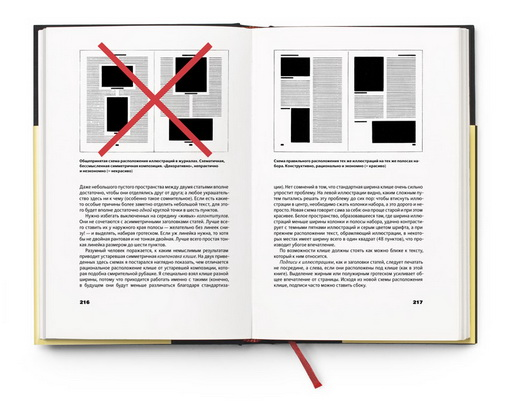
\includegraphics[width=0.95\textwidth]{tchichold01}
  \caption{\protect\url{http://www.artlebedev.com/everything/izdal/novaya-tipografika/}}
\end{figure}

\section{Technical discussion}
\subsection{The LaTeX standard classes}

LaTeX has pre-build layouts that depend  on two variables, specified by the user: the \textit{paper size} and the \textit{font size}. Appropriate values for the rest of the page layout are then  calculated by the class algorithm or are preset to certain values.

\subsection{Other common classes}

The more generic classes such as memoir and koma-script offer extensive customization and calculation of page parameters. They all use the basic laTeX page terminology which they supplement for additional parameters.

The octavo class offers a set of paper sizes suited for classical layouts printed on classical sizes such as the octavo. Classes such as the tufte-book offer a fixed design and no special commands for parameter manipulation.

\subsection{Paper sizes}

Most people using LaTeX, will print on either a4paper or letterpaper sizes. If you going to bind the work it might be necessary to trip the paper a little bit during binding to make sure that the top and side of the book are not ragged. This is normally called the \textit{trim}. If the document is to be printed by a publishing house this might be done by the printer which will use a different size \textit{stock size}. They might also allow for two additional dimensions called the spinemargin or the foremargin.

\begin{table}[ht]
\caption{North American paper sizes.}
\begin{tabular}{lllll}
\toprule
Size &width (mm)  &Height (mm)  &Width (in) &Height (in)\\
\midrule
US Ledger   &432 &279 & 17.0 &11.0\\
US Tabloid &279 & 432 & 11.0 &17.0\\
US Letter  &216 & 279 & 8.5 &11.0\\
US Legal   &216 &356 & 8.5 & 14.0\\
Government Letter &203 & 267 & 8.0 &10.5\\
Junior Legal &203 & 127 & 8.0 & 5.0\\
\bottomrule
\end{tabular}
\end{table}

\clearpage

\begin{table}[ht]
\caption{A series paper sizes.}
\begin{tabular}{lllll}
\toprule
Size &width (mm)  &Height (mm)  &Width (in) &Height (in)\\
\midrule
A0   &841 &1189 &33.1 & 46.8\\
A1   &594 & 841 &23.4 & 33.1\\
A2   & 420 & 594 &16.5 &23.4\\
A3   &297 & 420 &11.7 &16.5\\
A4   &210 &297 &8.3 &11.7\\ 
A5   &148 & 210 &5.8 & 8.3\\
A6   &105 & 148 & 4.1 & 5.8\\
A7   & 74 & 105 & 2.9 & 4.1\\
A8   &52 & 74 & 2.0 & 2.9\\
A9   &37 & 52 & 1.5 & 2.0\\
A10  & 26 & 37 & 1.0 & 1.5\\
\bottomrule
\end{tabular}
\end{table}


\begin{table}[ht]
\caption{ANSI series paper sizes.}
\begin{tabular}{lllll}
\toprule
Size &width (mm)  &Height (mm)  &Width (in) &Height (in)\\
\midrule
ANSI A &216 &279 &8.5 &11.0\\
ANSI B &279 &432 &11.0 &17.0\\
ANSI C &432 &559 &17.0 &22.0\\
ANSI D &559 &864 &22.0 &34.0\\
ANSI E &864 &1118 &34.0 &44.0\\

\bottomrule
\end{tabular}
\end{table}

\clearpage

\section{Swedish Standard}
The Swedish standard SIS 014711 generalized the ISO system of A, B, and C formats by adding D, E, F, and G formats to it. Its D format sits between a B format and the next larger A format (just like C sits between A and the next larger B). The remaining formats fit in between all these formats, such that the sequence of formats A4, E4, C4, G4, B4, F4, D4, H4, A3 is a geometric progression, in which the dimensions grow by a factor 21/16 from one size to the next. However, the SIS 014711 standard does not define any size between a D format and the next larger A format (called H in the previous example). Of these additional formats, G5 and E5 are popular in Sweden for printing dissertations,but the other formats have not turned out to be particularly useful in practice and they have not caught on internationally.

\begin{table}[ht]
\caption{Swedish Extension}
\begin{tabular}{lllll}
\toprule
Size &width (mm)  &Height (mm)  &Width (in) &Height (in)\\
\midrule
G5 &169 &239 &6.65 &9.41\\
E5  &155 &220 &6.10 &8.66\\

\bottomrule
\end{tabular}
\end{table}


\begin{table}
\centering
\caption{Octavo page layout parameters, influenced by font-size}
\begin{tabular}{llll}
\toprule
                    & 10pt & 11pt &12pt \\
\midrule
\textit{Octavo}              &      &      &\\
headsep        &  6pt  &  7pt &  8pt\\
topskip          & 10pt &  11pt & 12pt\\
texwidth         &0.7paperwidth & &\\
\midrule
\textit{LaTeX}              &      &      &\\
headsep        & .25in   &  .275in & .275in \\
topskip          & 10pt &  11pt & 12pt\\
footskip         &.35in &  .38in & 30pt \\
maxdepth         &.5\textbackslash topskip & &\\
textwidth        & 345pt  & 360pt & 390pt\\
\bottomrule
\end{tabular}
\end{table}

\subsection{The page dimensions}

The page dimensions are shown in figure 1. We tried to cater for the common terminology of all the classes.

\subsection{Texwidth}

The width of the text can only be determined based on the designer's strategy and is inexorably tied also to
the textheight. For example in classical page design, the designer tried to get the textwidth to be the same size like the page width, thus giving an almost squarish look. Another strategy is the 6-9 strategy, where the paper is divided into a grid of 9 equal blocks and the textwidth occupies the 6. 

\subsection{Readability considerations}

An average line that is longer than 40 to 70 characters long -- inluding spaces, is difficult to read. This is generally applicable to European languages and might be different for other languages. In addition the average number of words in one line should also be considered. For the German language Willi Egger (2004) recommends a line consisting of 8 to 12 words as optimal. If this strategy is adopted one can determine the line length based on the number of letters.

The characters per line for this document is \charactersperline. Of course from a readabilty point of view one could keep increasing the font size, but this is poor strategy. A well designed page should allow for good proportions as well as readabilty. In general a tolerance up  to 80 characters on a line should be adequate.

Peter Wilson in the manual for the memoir class refers to equations developed by Morten H{\o}gholm\index{H{\o}gholm, Morten} that has done some curve fitting
to the data. He determined that the expressions
\begin{equation}
L_{65} = 2.042\alpha + 33.41 \label{eq:L65}
\end{equation}
and
\begin{equation}
L_{45} = 1.415\alpha + 23.03 \label{eq:L45}
\end{equation}
fitted aspects of the data, where $\alpha$ is the length of the alphabet
in points, and $L_{i}$ is the suggested width in points, for a line with
$i$ characters (remember that 1pc = 12pt).

Using these equations one could get a first estimate of the textwidth. I am not too sure though if this is a good strategy as one can calculate it fully using TeX. bringhurst and them had to read these values from tables, but we do not; we can easily calculate them. For example to calculate the alphabet length for the bookman font:

\begin{texexample}{}{}
  \bgroup
  \fontfamily{pbk}\selectfont\alphabetlength\\
  \charactersperline\\
  \the\textwidth
  \egroup
\end{texexample}

Table~\ref{tab:alphlengths} adapted from the memoir class, gives alphabet lengths in points for various
fonts. My own recommendation is that for wide paper you should use a wider font and possibly move to 11pt font, rather than the traditional LaTeX default of 10pt.

\begin{table}
\centering
\caption{Lowercase alphabet lengths, in points, for various fonts}\label{tab:alphlengths}
\begin{tabular}{lrrrrrrrr} \toprule
                                            & 8pt & 9pt & 10pt & 11pt & 12pt & 14pt & 17pt & 20pt \\ \midrule
\fontfamily{pbk}\selectfont Bookman         & 113 & 127 & 142 & 155 & 170 & 204 & 245 & 294 \\
\fontfamily{bch}\selectfont Charter         & 102 & 115 & 127 & 139 & 152 & 184 & 221 & 264 \\
\fontfamily{cmr}\selectfont Computer Modern & 108 & 118 & 127 & 139 & 149 & 180 & 202 & 242 \\
\fontfamily{ccr}\selectfont Concrete Roman  & 109 & 119 & 128 & 140 & 154 & 185 & 222 & 266 \\
\fontfamily{pnc}\selectfont New Century Schoolbook     & 108 & 122 & 136 & 149 & 162 & 194 & 234 & 281 \\ 	
\fontfamily{ppl}\selectfont Palatino        & 107 & 120 & 133 & 146 & 160 & 192 & 230 & 276 \\ 	
\fontfamily{ptm}\selectfont Times Roman     &  96 & 108 & 120 & 131 & 143 & 172 & 206 & 247 \\
\fontfamily{put}\selectfont Utopia          & 107 & 120 & 134 & 146 & 161 & 193 & 232 & 277 \\
\fontfamily{pag}\selectfont Avant Garde Gothic  & 113 & 127 & 142 & 155 & 169 & 203 & 243 & 293 \\
\fontfamily{cmss}\selectfont Computer Sans  & 102 & 110 & 120 & 131 & 140 & 168 & 193 & 233 \\
\fontfamily{phv}\selectfont Helvetica       & 102 & 114 & 127 & 139 & 152 & 184 & 220 & 264 \\
\fontfamily{pcr}\selectfont Courier         & 125 & 140 & 156 & 170 & 187 & 224 & 270 & 324 \\
\fontfamily{cmtt}\selectfont Typewriter     & 110 & 122 & 137 & 149 & 161 & 192 & 232 & 277 \\
\bottomrule
%\facesubseeidx{Bookman}\facesubseeidx{Charter}\facesubseeidx{Computer Modern}%
%\facesubseeidx{Concrete Roman}\facesubseeidx{New Century Schoolbook}
%\facesubseeidx{Palatino}\facesubseeidx{Times Roman}\facesubseeidx{Utopia}%
%\facesubseeidx{Avant Garde Gothic}\facesubseeidx{Computer Sans}
%\facesubseeidx{Helvetica}\facesubseeidx{Courier}%
%\facesubseeidx{Computer Typewriter}%
\end{tabular}
\end{table}

\subsection{Textwidth influenced by margin materials}

Many books, including LaTeX allow for margin materials. If this is true then of course margins must by their nature be larger at the paper edges to allow for such material. 

\subsubsection{Simple strategy}
However, despite most of the above typesetting strategies many an author just want to take an approach, where they specify the margins and want to get what they need for example a spine margin of 1cm and an edge margin of 1.5cm. This is also important for screen dimensions.

\begin{lstlisting}
\cxset{
    margin inner= 1in
    margin outer= 2in
    margin top=1in
    margin bottom=2in
}
\end{lstlisting}

If all four margins are specified, the typesetting area can be positioned on the paper block. Life is not this easy though.

\begin{lstlisting}
\cxset{
    textarea proportional={1}{6}{2}  %
    textarea octavo
    textarea latex
    textarea other
}
\end{lstlisting}

\subsection{Auto strategy}

A more involved approach is to combine the strategies. First to get a good margin to type area, you will need to choose a paper that has good ratios. A paper such as \textit{imperial} comes close to an A4 size or imperial size. One can trip the balance of the paper or adjust slightly the ratios for twoside printing. Since we talking about book design any consideration for one side printing is immaterial. For oneside printing one can accept a wider latitude of values. Algorithm follows:

\begin{enumerate}
\item select paper.
\item select font.
\item marginmaterial true or false.
\item financial constraints - minimize number of pages, maximize number of pages.
\item check ideal number of characters at 65 per line.
\item decide on 10pt, 11pt or 12pt and constrain the algorithm.
\item use 0.7 textwidth area and check for max characters, if not iterate to 11pt.
\item recommend trimming values to suit.
\end{enumerate}


\subsection{Textheight}
Normally there is more latitude in choosing the 
proportions\index{proportion!margin} 
of the upper and lower margins, though usually the upper 
margin\index{margin!upper} is less than the lower margin\index{margin!lower}
so the typeblock\index{typeblock!location} is not vertically centered. Many modern books disregard all these rules and in many examples the upper margin is higher than the lower margin.

For text height calculations there are two considerations. One is to select top and bottom margings that are either equal or at a 1:1.5--2.0 ratio and relate to the width of the horizontal margins. The second consideration is that this length must be exactly divisible by baselineskip. When using \cs{flushbottom} LaTeX expects that the \cs{textheight} is such that a number of textlines in the body font will fit exactly into the height. If not, it issues an underfull vbox's message. LaTeX calculates these parameters when loading the class .clo files and sets the number of lines to a round number.

Many modern books have equal upper and lower margins.
\bigskip

\section{Allowing for trims}

Once a book is printed the edges are trimmed a bit in order to ensure a smooth top and right edge. For most desktop publishing you should not worry about such trimming. If you are going to publish the book in a professional publisher get their advice as to any allowances, you need to make in your pdf file. In other possible scenarios is that you may want to use a paper size such as A4 and trim it yourself down to one of the classical sizes such as Royal. 

All calculations are based on selecting a paper size and trimming it down. Unlike some other classes we assume you have selected the paper as stock size and then trimmed. Adding the trims makes no sense. You could simply print them on the larger page with trim marks, which we cater for.

  \begin{align}
   H_p    & = \sum h_1\ldots h_n\\
      h_t  &= H_p -   \sum h_1\ldots h_n - h_b
  \end{align}

The top margin is influenced by the \textit{device margin}, which is set at one inch, which we denote as $C$. If paper is to be trimmed the effective device margin offset will be reduced by the trim amount, $\Delta_t$.

Hence, the top margin is given by
\begin{align}
     h_t = C-\Delta_t+h1+h_2+h_3
\end{align}


\drawtriallayout


\printgeometryvalues
\readability

\newpage

\drawtriallayout

\readability

\newpage



% end of two page spread
\subsection{Top and bottom margins}

Before you follow any advice in places such as the Lulu forums to have your top and bottom margins equal, consider the following quotation by Bernard Shaw:

\begin{quotation}
Every printer can understand regularity: few have studied good looks except in living creatures. Consequently they aim at equal margins; and even when they have learnt that an upper margin must be less than a lower one if it is not to look more, they do not always see that it looks well only when it looks less. The mediaeval manuscript or early printed book, with its very narrow margin at the top and very broad margin at the bottom of the page, with its outer margins broad and its inner ones contracted, so that when the book lies open the two pages seem to make but a single block of letterpress in a single frame, instead of two side by side, has never been improved upon and probably never will be. But I find it almost impossible to persuade a modern printer to make his top margin small enough; and when I at last succeed, he measures it from the running title instead of from the top line of the page.

I saw a book the other day, excellently printed in old faced type, set solid, on a fine light, clean white crusty paper; yet the page was quite spoiled by an exaggerated top margin,like a masher's collar, and by that abomination of desolation, a rule. The only thing that never looks right is a rule. There is not in existence a page with a rule on it that cannot be instantly and obviously improved by taking the rule out.
\end{quotation}

\subsection{Headers and footers}
A page may have two additional items, and usually has at least one of these. They are the
running header and running footer. If the page has a folio then it is located either in the
header or in the footer. The word ‘in’ is used rather lightly here as the folio may not be
actually in the header or footer but is always located at some constant relative position. A
common position for the folio is towards the fore-edge of the page, either in the header or
the footer. This makes it easy to spot when thumbing through the book. It may be placed
at the center of the footer, but unless you want to really annoy the reader do not place it
near the spine.

Often a page header contains the current chapter title, with perhaps a section title on
the opposite header, as aids to the reader in navigating around the book. Some books put
the book title into one of the headers, usually the verso one, but I see little point in that as
presumably the reader knows which particular book he is reading, and the space would
be better used providing more useful signposts.

\subsubsection{Determining the geometry of the headers and footers}

The important parameter in the calculation of the header and footers, is the \cs{headheight} and \cs{headsep}. Most classes tend to have these as fixed parameters, related to font-size as can be seen in Table~\ref{tab:headerparams}.

\begin{table}[htbp]
\centering
\caption{Header and footer parameters settings by common classes.}
\label{tab:headerparams}
\begin{tabular}{llll}
\toprule
                    &headsep                   &headheight &footskip\\
\midrule
LaTeX 10pt    &             &                 &           \\
LaTeX 11pt    &             &                 &           \\
LaTeX 12pt    &             &                 &           \\
Octavo          &             &                 &           \\
tufte-book     &2 \texttt{baselineskip}   & 1 baselineskip           &            \\
\bottomrule
\end{tabular}
\end{table}

\begin{figure}[htbp]
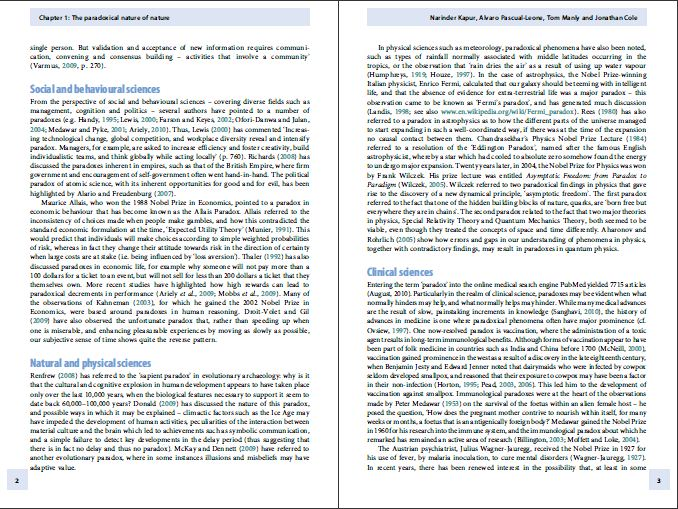
\includegraphics[width=\textwidth]{paradoxicalbrain}

\caption{Modern book approach to footer and header design. From \textit{Paradoxical Brain,} Narinder Kapur \textit{et al.}, Cambridge Univerity Press, 2011. Book is printed on Royal size paper.}
\label{fig:paradoxical}
\end{figure}

\begin{figure}[htbp]
{{\parindent0pt
\begin{tikzpicture}[inner sep=0pt,outer sep=0pt]
  \node (img) {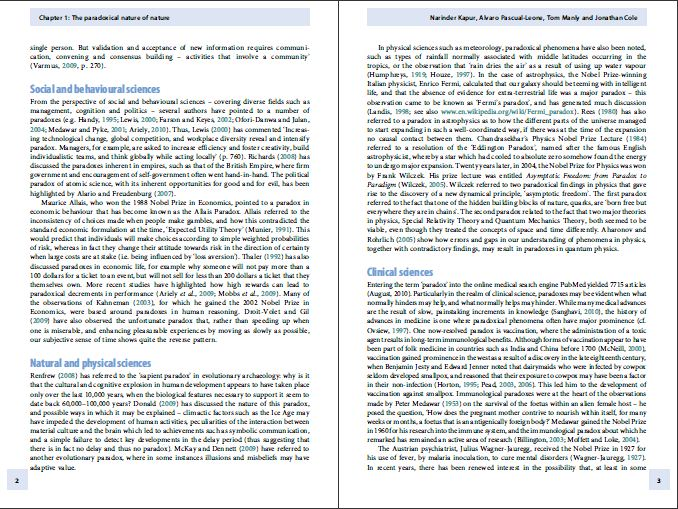
\includegraphics[height=8cm]{paradoxicalbrain}};
  \draw  (img.north east) ++ (5pt,0pt)-- ++ (15pt,0) ++(-15pt, -0.083*8cm) --++ (15pt,0pt) 
            (img.south east) ++ (5pt,0pt) -- ++ (15pt,0pt) ++ (0,0.075*8cm) -- ++ (-15pt,0);
\end{tikzpicture}}}
\caption{Modern book approach to footer and header design. From \textit{Paradoxical Brain,} Narinder Kapur \textit{et al.}, Cambridge Univerity Press, 2011. Book is printed on Royal size paper. The top margin is $1/12$ of the page height and the bottom margin is $1/16$ of page height. No need for apogryphal methods here.}
\label{fig:paradoxical}
\end{figure}

The more modern style tends to shift the headers and footers towards the top edge and bottom edge of the paper respectively, and allows very little space at the top of the paper. Figure~\ref{fig:paradoxical} shows a footer that is very near the bottom of the text and a header that has been shifted upwards. This makes for a more economical design as it increases the amount of text that can be printed in the typed area. For special designs such as this, it is not possible to automate calculations other than specifying a full algorithm for margins and typed area. Margins for the example follow the 10/12 rule for the typed area and inner and outer margins are equal at 1:12 ratio to the trimmed paper width.


\section{Floating parameters}


\section{Summing up}

Although one would ideally like to input some constraints and get out a perfect layout, as the previous discussion shows this is not an easy task, as well 

\begin{figure}[htbp]
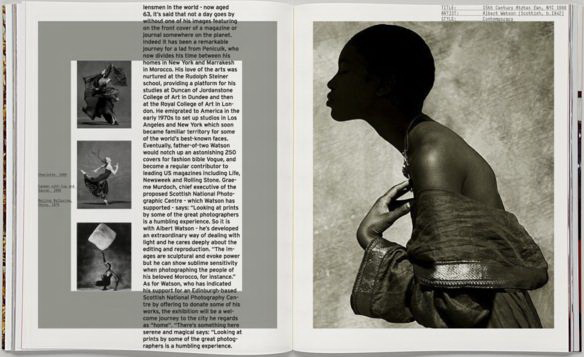
\includegraphics[width=0.9\textwidth]{artbook}
\end{figure}

%%\end{document}
%\lipsum[1-4]\marginnote[1pt]{\lorem
%    \lorem}
%
%\lipsum[1-2]

%% Stick the caption in the head might as well place the first picture also
\def\asidecaption{\parbox{4.2cm}{{\bfseries Image \thefigure}\par\lorem}%
  % \addtocontents{lof}{This is image 8}
}
\def\ps@caption{%
     \let\@oddfoot\@empty\let\@evenfoot\@empty%
    \def\@evenhead{%
        \begin{picture}(0,0)%
           \put(-150,-80){\asidecaption\par}%
            \stepcounter{figure}
           \put(-150,-370){\asidecaption}%
        \end{picture}%
      }%
    \let\@oddhead\@evenhead%
    \let\@mkboth\@gobbletwo%
    \let\chaptermark\@gobble%
    \let\sectionmark\@gobble%
 }

\def\ps@bigpicture{%
    \setlength\headheight{19cm}%
    \let\@oddfoot\@empty\let\@evenfoot\@empty%
    \def\@evenhead{%
         \begin{picture}(0,0)%
          \put(-149,0){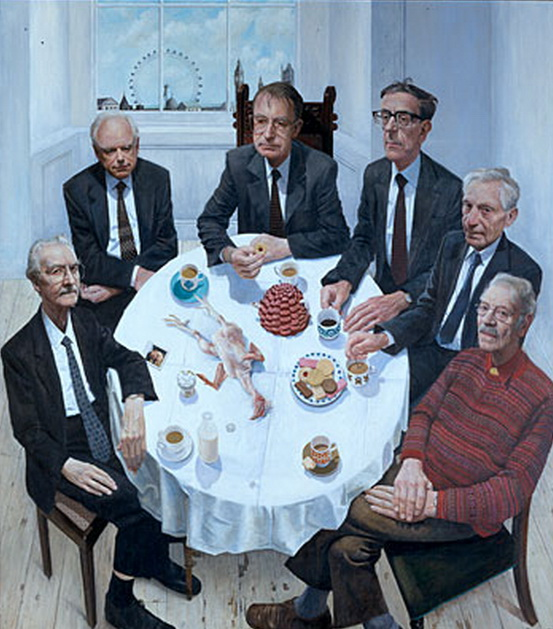
\includegraphics[width=\dimexpr(\textwidth+150pt)]{stuartpearson}}%
         \end{picture}%
      }%
    \let\@oddhead\@evenhead%
    \let\@mkboth\@gobbletwo%
    \let\chaptermark\@gobble%
    \let\sectionmark\@gobble%
 }



\def\doubletakeimage{%
  \renewcommand{\topfraction}{.95}  % ensure seecond image will not float away
  \begin{figure}[t]
    \thispagestyle{caption}
    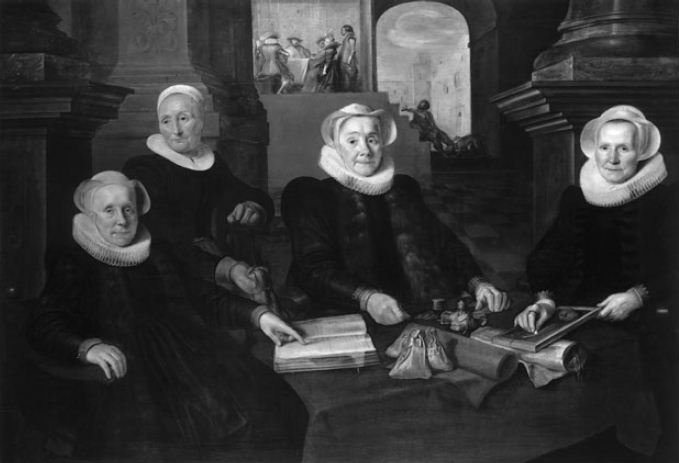
\includegraphics[width=\textwidth]{matron}%
  \end{figure}

  \begin{figure}[tp]
   \hspace*{-\marginparwidth}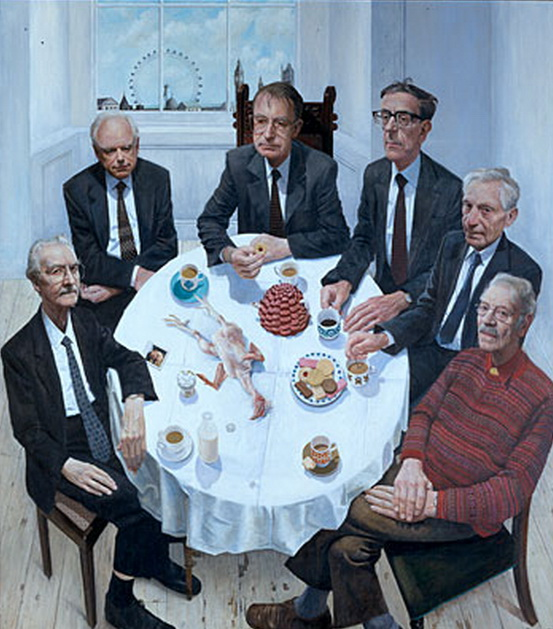
\includegraphics[height=0.9\textheight]{stuartpearson}
 \end{figure}
}




\lipsum[1-4]
\begin{figure}[htp]
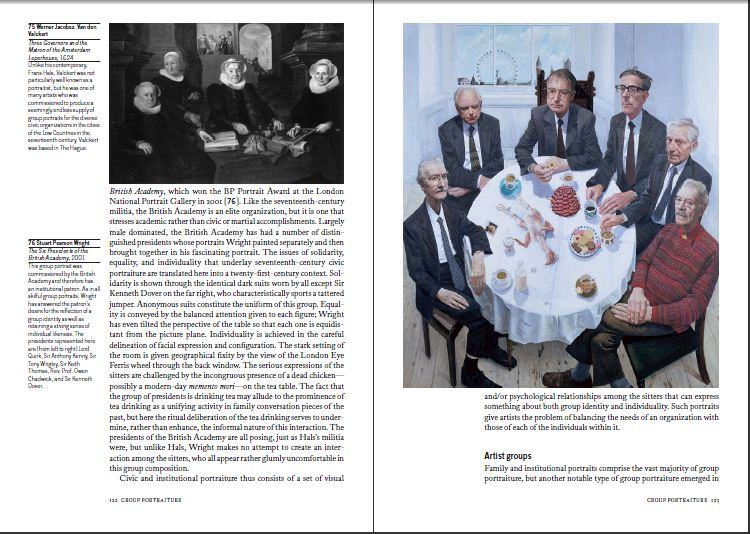
\includegraphics[width=0.98\textwidth]{captionspecial}
\centering
\caption{Figure from \textit{Oxford History of Art, Portraiture}, Shearer West, Oxford University Press, 2004. The figures are numbered consecutively and the text in the List of Illustrations have different formatting.}
\end{figure}

\doubletakeimage



%% RESET EVERYTHING AT END OF CHAPTER
\addtocounter{chapter}{-2}

\@toctrue\@specialtrue

%\@specialfalse
\pdfpageheight=\paperheight
\pdfpagewidth=\paperwidth
\cxset{manet, toc image=false}
\cxset{toc image=false},
\topimage{manet}

\chapter{THE BARMAID}
\begin{multicols}{3}
      \leftskip0pt
      \lettrine{I}{psum dolor} sit amet latixeus. \lipsum*[1-2]
      Latinicus porcupinus to fill the line.
      \tikz{\draw[thick] (0,0)--(\columnwidth,0);}
\end{multicols}
\clearpage


%\cxset{manet, toc image=false}
%\cxset{toc image=false},
%\topimage{Alan-MacDonald-Cardinal-Spin-01}
%\chapter{THE BARMAID}
%\begin{multicols}{3}
%      \leftskip0pt
%      \lettrine{I}{psum dolor} sit amet latixeus. \lipsum*[1-2]
%      Latinicus porcupinus to fill the line.
%\end{multicols}
%\clearpage
%\@specialfalse


\newgeometry{top=1.35cm,bottom=2cm,left=2cm}
\clearpage
\cxset{manet/.style={
 chapter opening=anywhere,
 chapter toc=true,
 toc image=false,
 name={},
 numbering=none,
 number font-size=,
 number font-family=,
 number font-weight=,
 number before={\vspace*{-2.5cm}},
 number dot={},
 number after={},
 number position=leftname,
 chapter font-family=,
 chapter font-weight=,
 chapter font-size=,
 chapter before=,
 chapter after={},
 chapter color={black!90},
 number color= teal,
 title beforeskip={},
 title afterskip={},
 title before={\hspace*{-2.47cm}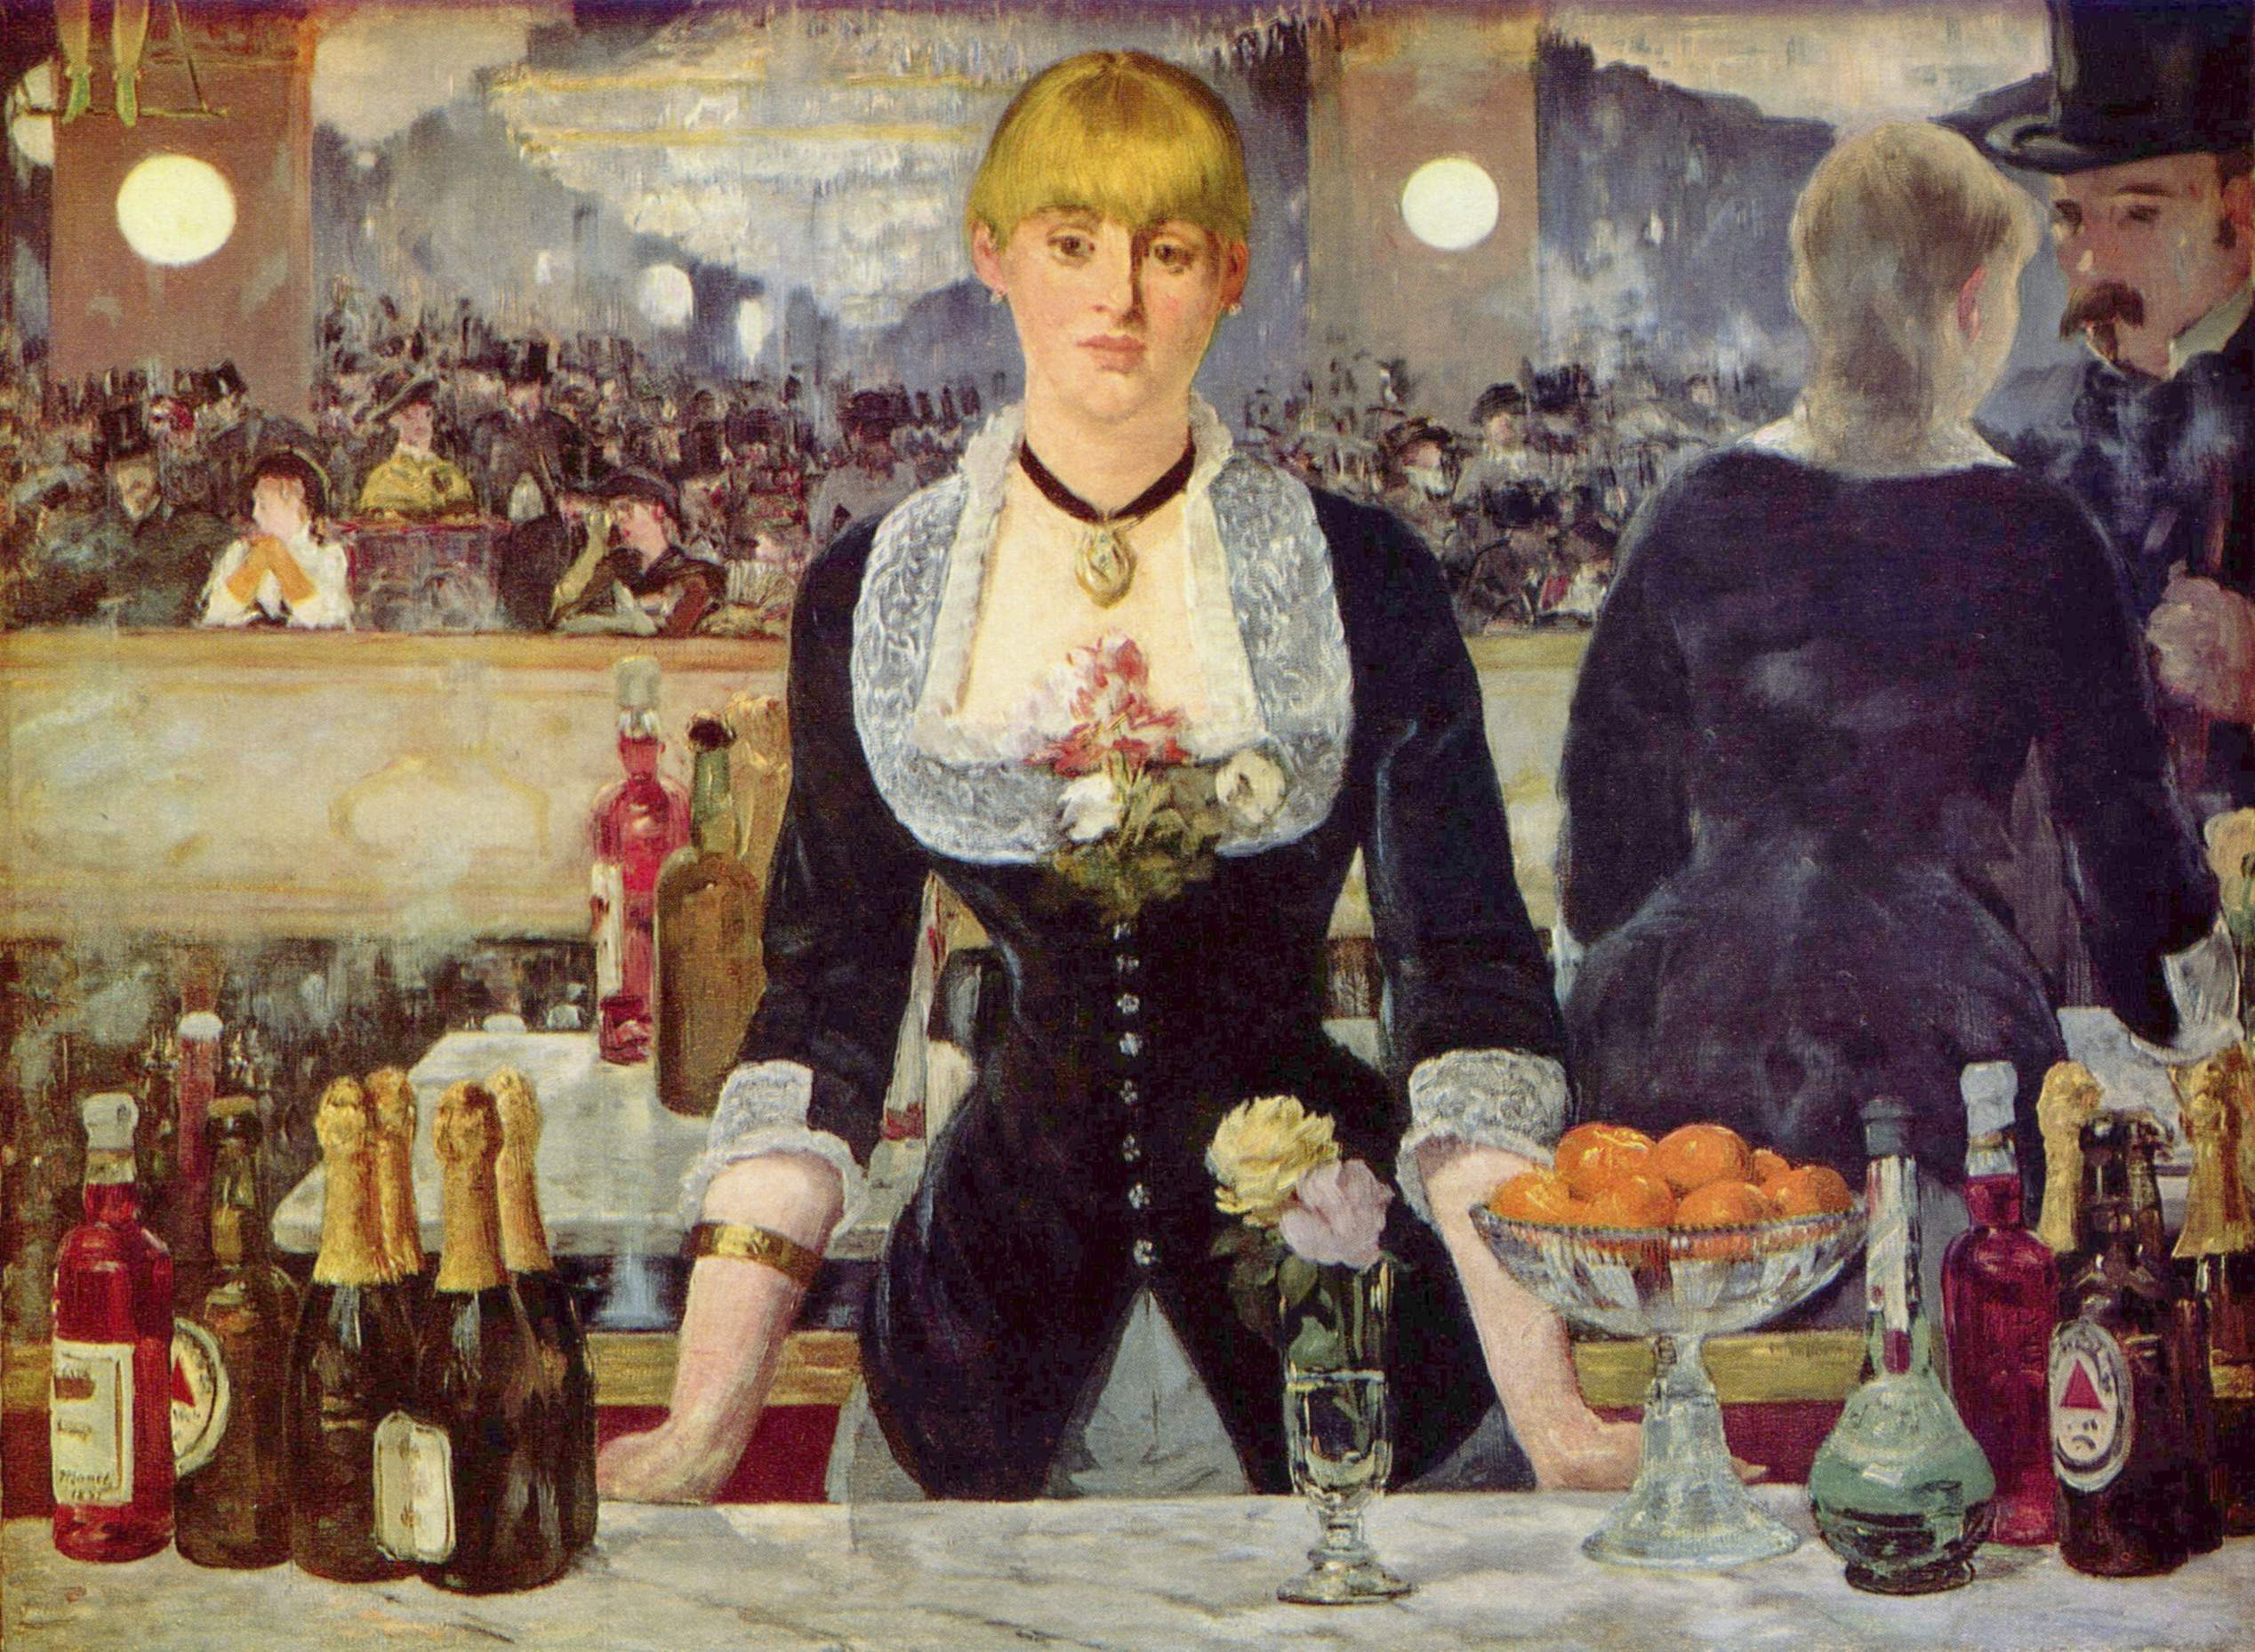
\includegraphics[width=1.27\textwidth]{./chapters/manet}%
    \par\hfill\hfill{\tiny\bfseries Manet's  \textit{The Barmaid.}}\\
    \par
    \vspace*{\baselineskip}
    \par\hfill},
 title after={\hfill\hfill},
 title font-family=\sffamily,
 title font-color= black!80,
 title font-weight=\bfseries,
 title font-size=\LARGE}}
\cxset{manet}



\chapter{A New Approach to Designing \LaTeX\ Classes}
\begin{multicols}{3}
      \leftskip0pt
      \lettrine{I}{psum dolor} sit amet latixeus. \lipsum*[1-2]
      Latinicus porcupinus to fill the line.


This particular code, uses the predefined style \textit{manet}. The only difference we have now defined a helper macro to make it easier for such images to be inserted for similar style chapter openings.
If a full book is to be designed using chapter openings in this fashion more keys and styles could be defined to make it even more easy to enter.
\end{multicols}



\def\topimage#1{\cxset{title before={\hskip-2.3cm\includegraphics[width=1.25\textwidth]{./chapters/#1}\par
\vspace*{\baselineskip}\par}}}




The full code to have the chapter typeset is shown below:


\begin{lstlisting}
\cxset{manet}
\topimage{Alan-MacDonald-Cardinal-Spin-01}

\chapter{ALAN MacDONALD}
\begin{multicols}{3}
      \leftskip0pt
      \lettrine{I}{psum dolor} sit amet latixeus. \lipsum*[1-2]
      Latinicus porcupinus to fill the line.
\end{multicols}
\end{lstlisting}
\lipsum[2]

\loadgeometry{std}



%\cxset{toc image=false},

\long\gdef\versochapter#1{%
  \vspace*{3cm}
  \minipage{\textwidth}
  \hfill\includegraphics[width=0.63\textwidth]{\chapterimage@cx}\par
  \vspace*{6pt}
  \hfill\minipage{0.75\textwidth}
  {\HUGE\bfseries\flushright #1\endflushright}
  \endminipage
  \endminipage
  \newpage


\vspace*{10cm}
\@specialfalse
\@openleftfalse
\@openanyfalse
\@openrighttrue
}


\newgeometry{bottom=2.5cm}

\cxset{
   chapter image/.code={\def\chapterimage@cx{#1}},
   chapter opening/.is choice,
   chapter opening/verso/.code={\@specialtrue\@openlefttrue
   \gdef\customdesign@cx##1{\versochapter{##1}}}
}

\cxset{
 chapter image=onesowndeath,
 chapter opening=verso,
 name={},
 numbering=none,
 number font-size=\LARGE,
 number font-family=\rmfamily,
 number font-weight=\bfseries,
 number before=,
 number dot=,
 number after=,
 number position=leftname,
 chapter font-family=\sffamily,
 chapter font-weight=\normalfont,
 chapter font-size=\Large,
 chapter before={\vspace*{0pt}\par},
 chapter after={\hfill\hfill\par},
 chapter color={black!90},
 number color=\color{purple},
 title beforeskip={\vspace*{0pt}},
 title afterskip={\vspace*{0.4\textheight}\par},
 title before={},
 title after={},
 title font-family=\sffamily,
 title font-color=\color{purple},
 title font-weight=\bfseries,
 title font-size=\LARGE,
 header style=plain,
 pagestyle=plain,
 }

\@specialtrue

\chapter[VERSO CHAPTERS]{Verso Chapters}

\parindent1.5em
{\HUGE V}erso chapter openings are not common. One design that I found quite attractive is \lipsum[1-3] \textit{From Western attitudes toward death from the middle ages to the present}, Philippe Ari\'es. London, 1974.

\begin{figure}
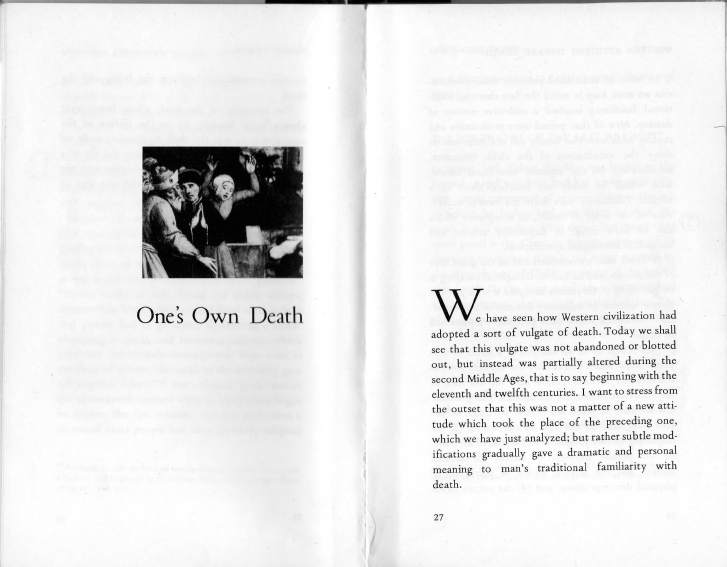
\includegraphics[width=\textwidth]{versochapter01}
\caption{Chapter opening on verso page.}
\end{figure}


%\makeatletter\@specialfalse

\cxset{
 toc image = \@empty,
 name={},
 numbering=arabic,
 number font-size= LARGE,
 number font-family= rmfamily,
 number font-weight= bfseries,
 number before=,
 number dot=,
 number after=,
 number position=leftname,
 chapter font-family= sffamily,
 chapter font-weight= normalfont,
 chapter font-size= Large,
 chapter before={\vspace*{15pt}\par},
 chapter after={\hfill\hfill\par},
 number color=black!90,
 title beforeskip={\vspace*{30pt}},
 title afterskip={\vspace*{40pt}\par},
 title before={},
 title after={},
 title font-family= sffamily,
 title font-color= black,
 title font-weight= bfseries,
 title font-size= LARGE,
 header style= plain,
 }

\cxset{headings ruled-01}

\chapter{Introduction to Style One}


\begin{summary}
This design is simple and its distinguishing characteristic is a short summary at the beginning of the chapter. This is almost like an abstract typeset in italic font without setting the margins in. We provide a \lstinline{summary} environment for convenience. Note the very simple line in the running head to the left of the page number.
\end{summary}

\medskip
\begin{figure}[ht]
\centering
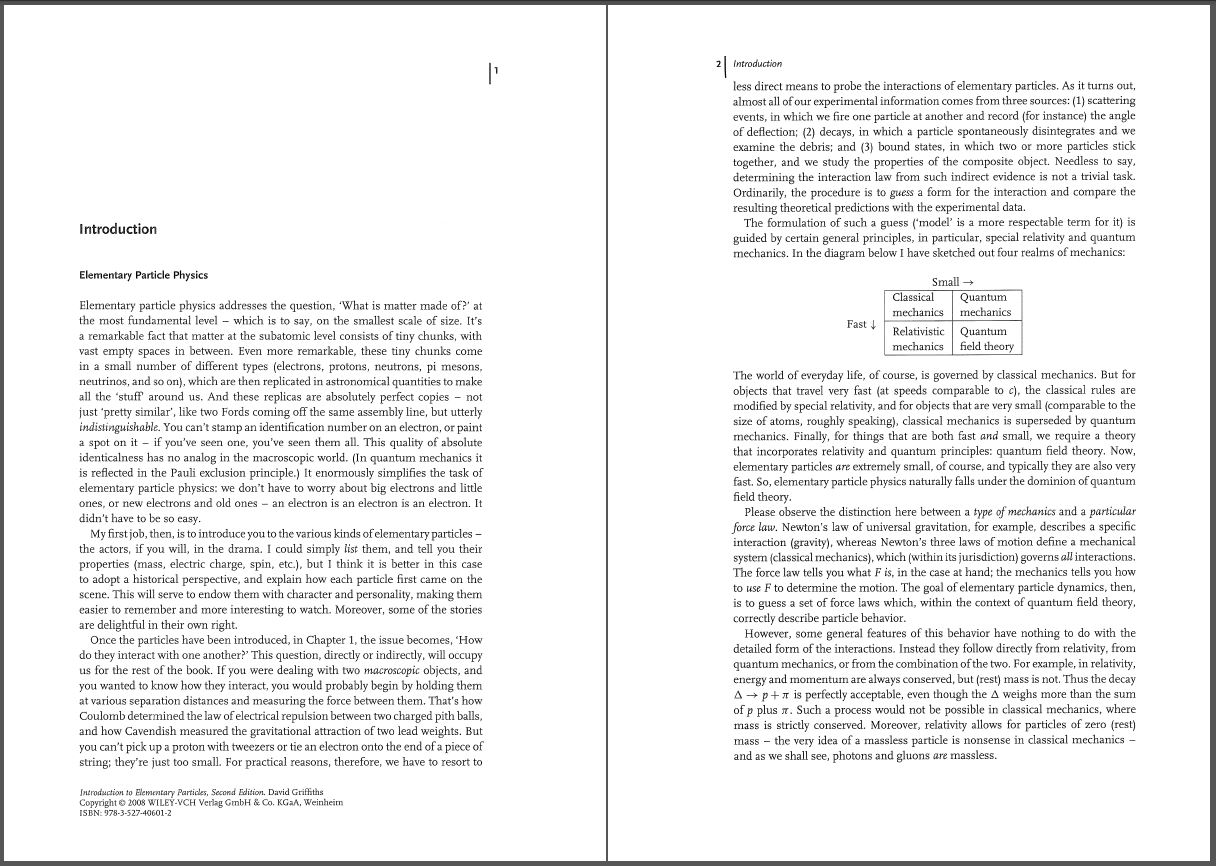
\includegraphics[width=0.5\textwidth]{./chapters/chapter01.png}
\end{figure}
\makeatother

%\clearpage
\makeatletter\@debugtrue\makeatother
\cxset{
 chapter toc=true,
 name=CHAPTER,
 chapter numbering=ORDINALS,
 number font-size=Large,
 number font-family=rmfamily,
 number font-weight=bfseries,
 number before=\kern0.5em,
 number dot=,
 number after=\hfill\hfill\par,
 number position=rightname,
 chapter font-family=rmfamily,
 chapter font-weight=bold,
 chapter font-size=Large,
 chapter before={\vspace*{20pt}\par\hfill},
 chapter after=,
 chapter color=black,
 number color=black,
 %
 title margin top=10pt,
 title before=\par\nointerlineskip\hfill,
 title after=\hfill\hfill\par\nointerlineskip,
 title font-family=rmfamily,
 title font-color= black,
 title font-weight=bfseries,
 title font-size=LARGE,
 chapter title width=0.8\textwidth,
 chapter title align=centering,
 title margin-left=0pt,
 author block=false}

\debugtitle
\debugchapter
\chapter[Template 2]{Mondino, the Restorer of Anatomy}

The archive.org is an extraordinary hunting ground  for typographical surprises. On a recent excursion to find some books on Versalius I stubled on a book titled \emph{Andreas Vesalius, the reformer of anatomy} by  Ball, James Moores. It is an old book published in 1910 and has a couple of unusual features. Check the figure below and see if you can identify the challenging feature.

\begin{figure}[ht]
\centering
\includegraphics[width=0.8\textwidth]{versalius}
\caption{J.B. Moore’s \emph{Andreas Versalius, the Reformer of Anatomy} has many unusual features, including chapter numbers using ordinals. }
\end{figure}

\cxset{chapter toc=true,
          chapter opening=anywhere}
          
\chapter{The Template}          
The template is called \emph{Versalius} and is stored under style02. It can be loaded in the normal way using:
\begin{verbatim}
\usepackage[style02]{phd}
\end{verbatim}

I have not reproduced the full extend of the book’s requirements, as some details are quite cumbersome to be automated through \tex. These though can easily be incorporated in a manual way. More about this later.


\section{The Table of Contents}
Another interesting aspect of this book, which is common with many books of its period is the ToC. The ToC shows the full range of the chapter pages, i.e., it is marked as Page 1-16 rather than the common practice nowdays that indicates only the starting page of the chapter. It also has “TABLE OF CONTENTS”  as a heading and not just contents as you would expect from today’s books.

\begin{figure}[ht]
\centering
\includegraphics[width=0.8\textwidth]{versalius-01}
\caption{J.B. Moore’s \emph{Andreas Versalius, the Reformer of Anatomy} has many unusual features, including chapter numbers using ordinals. }
\end{figure}

\section{List of Illustrations}

\begin{figure}[ht]
\centering
\includegraphics[width=0.8\textwidth]{versalius-02}
\caption{J.B. Moore’s \emph{Andreas Versalius, the Reformer of Anatomy} has many unusual features, including chapter numbers using ordinals. }
\end{figure}

\section{The Frontmatter}
As a foreward there is an unumbered chapter called ``Introduction’’. The chapter heading also has a head band.
\begin{figure}[ht]
\centering
\includegraphics[width=0.8\textwidth]{versalius-03}
\caption{J.B. Moore’s \emph{Andreas Versalius, the Reformer of Anatomy} has many unusual features, including chapter numbers using ordinals. }
\label{lettrine}
\end{figure}

\bgroup
\centering
\includegraphics[width=0.7\textwidth]{versalius-headband}

\LARGE\bfseries INTRODUCTION\par
\egroup
\def\dropcapversalius{%
\vbox to 0pt{\vskip6pt\leavevmode\noindent\includegraphics[width=2.39cm]{versalius-dropcap}%
}%
}
\parindent0pt

\hangindent2.6cm \hangafter0
\dropcapversalius \textsc{he dropcap will have to be inserted}, either using the lettrine package or do be achieved via a parshape command and manual entry. You can also write your own macro command using the details we provide under the Paragraphs chapter. On this page I have manually inserted it, as I used an image from the book for the dropcap. If you were to use the template for a full book, it will be then preferable to use

the lettrine package to set the dropcaps. If you observe Figure~\ref{lettrine} carefully, you will notice the first line of theopening paragraph is in small caps. As \tex typesets the full paragraph this is almost an impossible task to achieve through normal \tex commands and in order not to overcomplicate the discussion it can be achieved manually via trial and error. 

\section{Figures}

Most of the figures are wrapped illustrations. A couple are full page figures and bear no caption numbering. One such illustration is shown on page~\pageref{fig:vesalius}. Do note that the List of Illustrations does have the illustrations listed with additional information to that shown in the captions. 

\begin{figure}[p]
\centering
\includegraphics[width=\textwidth]{vesalius}
\centering
ANDREAS VESALIUS\par
(From an old copperplate engraving)\par
\label{fig:vesalius}
\end{figure}







%\newgeometry{top=-10pt,bottom=2cm}


\cxset{style03/.style={
 toc image = \@empty,
 name={},
 numbering=arabic,
 number font-size= HUGE,
 number font-family= rmfamily,
 number font-weight= bfseries,
 number before=\par\vspace*{10pt}\hfill\hfill,
 number dot=.,
 number after=,
 number position=rightname,
 chapter font-family= sffamily,
 chapter font-weight=normalfont,
 chapter font-size= Large,
 chapter before={\hspace*{-2.5cm}\vbox\bgroup%
    \tcbset{width=\paperwidth,boxrule=0pt,right=3cm,arc=0pt}
    \tcolorbox\bgroup\vspace*{20pt}\hfill\hfill},
 chapter after={\par\vspace*{15pt}},
 chapter color=black!90,
 number color= thered,
 title beforeskip={},
 title afterskip={\vspace*{10pt}\par},
 title before={\hfill\hfill},
 title after={\vspace*{60pt}\egroup\endtcolorbox\egroup},
 title font-family=\sffamily,
 title font-color= thered,
 title font-weight=\bfseries\RaggedRight,
 title font-size=\Huge}}

\cxset{style03}

\chapter{Introduction Style Three}

This is not an exact reproduction as I am still thinking as to how to use
specials with the package. You can vary it by setting the tcolorbox settings as well as the geometry settings.
\medskip

\begin{figure}[ht]
\centering

\includegraphics[width=0.39\textwidth]{./chapters/chapter03}
\end{figure}

This setting involves changing the geometry of the page as well as adding the chapter name and title in a color box. For this I have used the \lstinline{tcolorbox}. Of course you can use any other shaded environment you feel comfortable with such as mdframed. It is important to set the colorbox parameters.

\begin{lstlisting}
\newgeometry{top=-10pt}
\tcbset{width=\paperwidth,boxrule=0pt,right=3cm,arc=0pt}
\end{lstlisting}

Note that we set the width of the \lstinline{tcolorbox} to \lstinline{\paperwidth} in order for the shading to extend to the full width of the page.

\restoregeometry

%\cxset{style04/.style={
 chapter name=,
 numbering=Roman,
 number font-size=Large,
 number font-family=rmfamily,
 number font-weight=bfseries,
 number before=,
 number dot=,
 number after=,
 number color=black,
 number position=rightname,
 chapter font-family= rmfamily,
 chapter font-weight=bold,
 chapter font-size=Large,
 chapter before=,
 chapter after=,
 chapter color=black!90,
 chapter border-style=none,
 chapter border-width=0pt,
 chapter display=block,
 chapter float=center,
 title beforeskip={},
% title afterskip={\vspace*{50pt}\par},
 title margin bottom=50pt,
 title margin-left=0pt,
 chapter title align=centering,
 chapter title text-align=center,
 chapter title width=\textwidth,
 title display=block,
 title border-left-width=0.2pt,
% title hooks leave emptt 
 title before=,
 title after=,
 % title families leave as default font name
 title font-family=rmfamily,
  title font-color= black,
 title font-weight=normalfont,
 title font-size=LARGE,
 % title alignment
 chapter title align=centering,
 % sectioning incomplete please add to suit
 section numbering=none,
 section align = center}}

\debugchapter
\cxset{chapter border-width=2pt,
          chapter padding=5pt,
          number border-width=2pt,
          number padding=5pt}

\cxset{style04}

\chapter{INTRODUCTION TO STYLE FOUR}

This is a very simple design applicable perhaps to translations and commentary on older texts.
\medskip
\begin{figure}[ht]
\centering
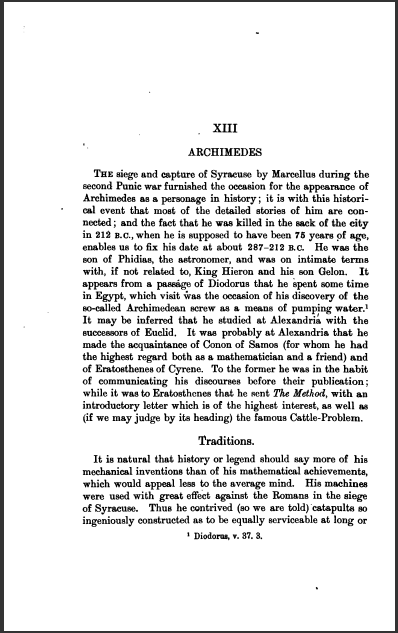
\includegraphics[width=0.6\textwidth]{./chapters/chapter04.png}
\end{figure}

\testsections



%%%%%%%%%%%%%%%%%%%%%%%%%%%%%%%%%%%%%%%%%%%%
%%%%%%  STYLE 05
%%%%%%%%%%%%%%%%%%%%%%%%%%%%%%%%%%%%%%%%%%%


\cxset{style05/.style={
 name={Chapter},
 numbering=arabic,
 number font-size=\Large,
 number font-family=\rmfamily,
 number font-weight=\normalfont\itshape,
 number color=\color{black!90},
 number before=,
 number dot=,
 number after=,
 number position=rightname,
 chapter font-family=\rmfamily,
 chapter font-weight=\normalfont\itshape,
 chapter font-size=\Large,
 chapter before={\hrule width \columnwidth \kern2.6pt \par\hfill},
 chapter after={\hfill\hfill\par},
 chapter color={black!90},
 chapter spaceout=none,
 title beforeskip={\vspace*{10pt}},
 title afterskip={\vspace*{50pt}\par},
 title before={\hfill},
 title after={\hfill\hfill \vskip2.6pt\hrule width \columnwidth \kern2.6pt },
 title font-family=\rmfamily,
 title font-color=\color{black!90},
 title font-weight=\bfseries,
 title font-size=\huge,
 header style= headings}}

\cxset{style05}
\chapter{Introduction to Style Five}\index{ch:style5}

\tcbset{width=\textwidth}
I think this style can be improved with a bit of color. You can experiment with it quite easily. The spacing on top of this style can also be adjusted to suit your typographical taste.
\medskip
\begin{figure}[ht]
\centering
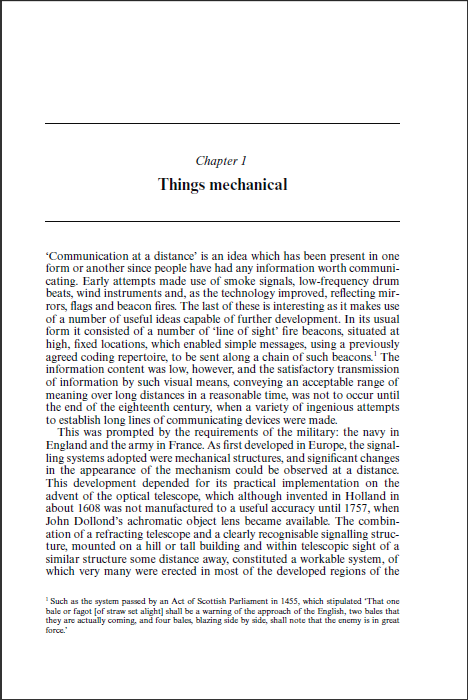
\includegraphics[width=0.6\textwidth]{./chapters/chapter05}
\end{figure}

%\section{General notes on rules}

LaTeX's default rules would normally give problems. Best is to use TeX's primitives to built them.

%\index{rules!example color}
%\begin{texexample}{}{}
%\makeatletter
%\hrule width 5cm \kern2.6\p@
%AAAAAAAAAAAAAAAAAAAAA
%\vskip2.6pt\hrule width 5cm
%\medskip
%
%Problem with LaTeX rules.
%
%\rule{5cm}{0.4pt}\par
%AAAAAAAAAAAAAAAAAAAAA\par%
%\rule[6.5pt]{5cm}{0.4pt}
%
%\def\rule{\@ifnextchar[\@rule{\@rule[\z@]}}
%\def\@rule[#1]#2#3{%
% \leavevmode
% \hbox{%
% \setlength\@tempdima{#1}%
% \setlength\@tempdimb{#2}%
% \setlength\@tempdimc{#3}%
% \advance\@tempdimc\@tempdima%
% \vrule\@width\@tempdimb\@height\@tempdimc\@depth-\@tempdima}}
%
%\def\thickrule{\leavevmode \leaders \hrule height 3pt \hfill \kern \z@}
%
%{\color{teal}\hrule width 10.5cm height3pt \kern2.6\p@
%    {{\color{black!80}\HUGE CHAPTER TITLE}}\vskip3pt
%\hrule width 10.5cm height3pt}
%\makeatother
%\end{texexample}

%<<<<<<< HEAD
%%%%%%%%%%%%%%%%%%%%%%%%%%%%%%%%%%%%%%%%%%%
%%%%%%  STYLE 06
%%%%%%%%%%%%%%%%%%%%%%%%%%%%%%%%%%%%%%%%%%%

\cxset{style06/.style={
 name={Chapter},
 numbering=arabic,
 number font-size=\Huge,
 number font-family=\calligra,
 number font-weight=\calligra,
 number color=\color{black!90},
 number before=\kern-2.5pt,
 number dot=,
 number after=,
 number position=rightname,
 chapter font-family=\rmfamily,
 chapter font-weight=\calligra,
 chapter font-size=\LARGE\calligra,
 chapter before={\vspace*{20pt}\par\hfill},
 chapter after={\hfill\hfill\par},
 chapter color={black!90},
 title beforeskip={\vspace*{50pt}},
 title afterskip={\vspace{3.5pt}\par},
 title before={\hfill},
 title after={\hfill\hfill},
 title font-family=\rmfamily,
 title font-color=\color{black!90},
 title font-weight=\normalfont,
 title font-size=\LARGE,
 title spaceout=soul,
}}

\cxset{style06}

\chapter{INTRODUCTION TO STYLE SIX}
\renewcommand{\DefaultLhang}{0.1}
\renewcommand{\LettrineFontHook}{\calligra}
\setlength{\DefaultFindent}{9.5pt}
\setlength{\DefaultNindent}{0pt}

\lettrine{\textcolor{orange}{T}}{}he calligraphic font for this design make it stand out, although you may need to experiment to get the right font (I have used calligra). I am sure the specification can be optimized a bit, however so far it works. I also opted to space out the title. I had to experiment a bit to get the Lettrine settings.
\medskip
\begin{figure}[ht]
\centering
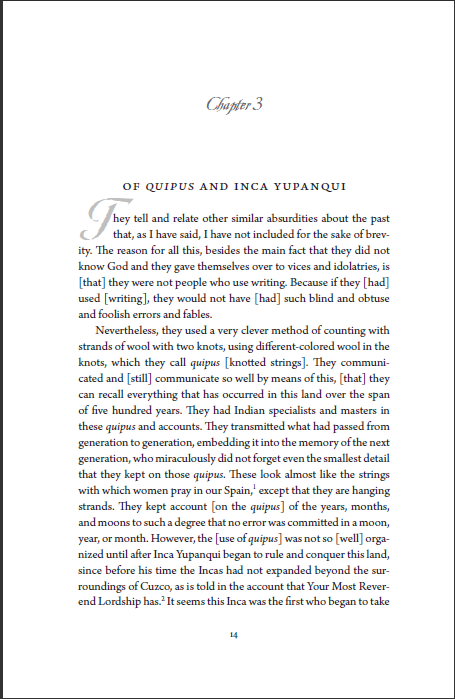
\includegraphics[width=0.6\textwidth]{./chapters/chapter06}
\end{figure}

The number has been kerned using:

\begin{lstlisting}
 number before=\kern-4.5pt,
\end{lstlisting}

This template has a lot of potential and I will come back to it and add more key hooks for lettrine settings per letter and font management. They can also come alive with a gold color.

=======
%%%%%%%%%%%%%%%%%%%%%%%%%%%%%%%%%%%%%%%%%%%
%%%%%%  STYLE 06
%%%%%%%%%%%%%%%%%%%%%%%%%%%%%%%%%%%%%%%%%%%

\cxset{style06/.style={
 name={Chapter},
 numbering=arabic,
 number font-size=\Huge,
 number font-family=\calligra,
 number font-weight=\calligra,
 number color=\color{black!90},
 number before=\kern-2.5pt,
 number dot=,
 number after=,
 number position=rightname,
 chapter font-family=\rmfamily,
 chapter font-weight=\calligra,
 chapter font-size=\LARGE\calligra,
 chapter before={\vspace*{20pt}\par\hfill},
 chapter after={\hfill\hfill\par},
 chapter color={black!90},
 title beforeskip={\vspace*{50pt}},
 title afterskip={\vspace{3.5pt}\par},
 title before={\hfill},
 title after={\hfill\hfill},
 title font-family=\rmfamily,
 title font-color=\color{black!90},
 title font-weight=\normalfont,
 title font-size=\LARGE,
 title spaceout=soul,
}}

\cxset{style06}

\chapter{INTRODUCTION TO STYLE SIX}
\renewcommand{\DefaultLhang}{0.1}
\renewcommand{\LettrineFontHook}{\calligra}
\setlength{\DefaultFindent}{9.5pt}
\setlength{\DefaultNindent}{0pt}

\lettrine{\textcolor{orange}{T}}{}he calligraphic font for this design make it stand out, although you may need to experiment to get the right font (I have used calligra). I am sure the specification can be optimized a bit, however so far it works. I also opted to space out the title. I had to experiment a bit to get the Lettrine settings.
\medskip
\begin{figure}[ht]
\centering
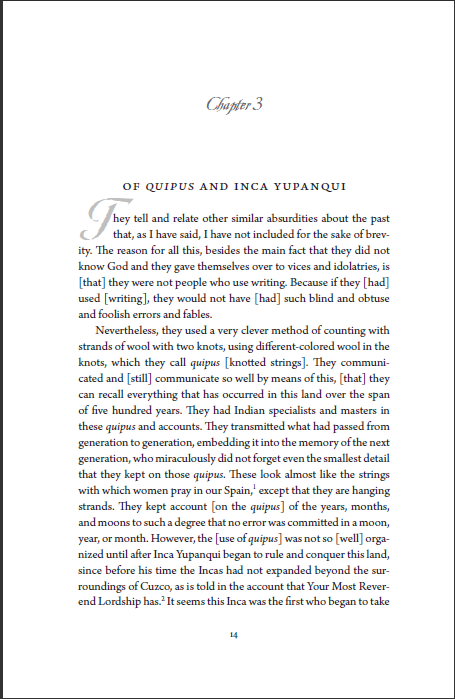
\includegraphics[width=0.6\textwidth]{./chapters/chapter06}
\end{figure}

The number has been kerned using:

\begin{lstlisting}
 number before=\kern-4.5pt,
\end{lstlisting}

This template has a lot of potential and I will come back to it and add more key hooks for lettrine settings per letter and font management. They can also come alive with a gold color.

>>>>>>> merged

%
\newgeometry{top=2cm,bottom=2cm,left=3cm,right=3cm}

\setdefaults

\cxset{style07/.style={
 name={},
 chapter toc=true,
 numbering=arabic,
 number font-size=HUGE,
 number font-family=sffamily,
 number font-weight=bfseries,
 number before=,
 number dot=,
 number color= gray,
 number after=\par,
 number position=leftname,
 chapter font-family=\sffamily,
 chapter font-weight=\normalfont,
 chapter font-size=\Large,
 chapter before={\hfill\hfill\hfill\par},
 chapter after={\vspace*{20pt}},
 chapter color= black!90,
 title beforeskip={\vspace*{30pt}},
 title afterskip={\vspace*{50pt}\par},
 title before={},
 title after={\par\rule[17pt]{\textwidth}{0.4pt}},
 title font-family=\sffamily,
 title font-weight=\bfseries,
 title font-size=\LARGE,
 title font-shape=normal,
 title font-color=black!90,
 title spaceout=none,
}}

\cxset{style07}
\chapter{Introduction to Style Seven}

\parindent0pt
\lipsum[1]
\medskip
\begin{figure}[ht]
\centering
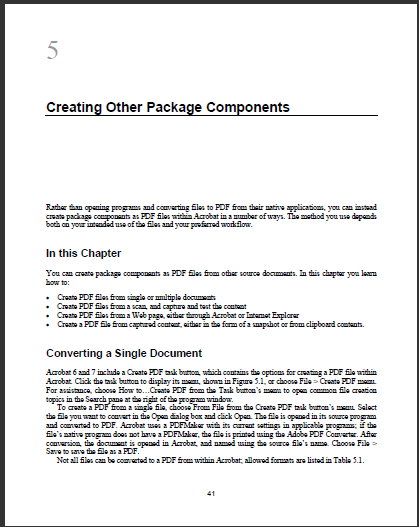
\includegraphics[width=0.6\textwidth]{./chapters/chapter07.png}
\end{figure}
\lipsum[1]

%\clearpage

\setdefaults

\makeatletter
\cxset{style08/.style={
 name={},
 chapter toc=true,
 numbering=arabic,
 number font-size=\LARGE,
 number font-family=\sffamily,
 number font-weight=\bfseries,
 number color= black!90,
 number before=,
 number dot=,
 number after=,
 number position=rightname,
 chapter font-family=sffamily,
 chapter font-weight=normalfont,
 chapter spaceout=none,
 chapter font-size=Large,
 chapter before=,
 chapter after=,
 chapter color={black!90},
 chapter float=right,
 chapter display=block,
 chapter border-style=none,
 chapter border-width=0pt,
 number spaceout=none,
 number display=block,
 number float=right,
 chapter title width=0.6\textwidth,
 title beforeskip=,
 title afterskip=,
 title before=,
 title after={},
 title font-family=sffamily,
 title font-color=black!90,
 title font-weight=bfseries,
 title font-size=LARGE,
 title display=block,
 chapter title align=right,
 author block=true,
 author block format=\par\addvspace{12pt}\normalfont\large\raggedleft,
 author names=Yiannis Lazarides\par Larnaka,
 section number after=,
 section numbering = arabic,
 section numbering prefix=,
 section numbering custom = \@arabic\c@section.\space,
 section color=black,
 section numbering suffix=,
 header style=empty}}
 
 % humanized name of the style, with a non human connotation!
 %
 \cxset{humanoid/.style={style08}}
\makeatother

\cxset{section color=sweet,
          section font-shape=sffamily}


\cxset{style08}
% set the counter needs this to be modified to be based on a key value interface
\cxset{figure numbering/.is choice,
          figure numbering/within/.code=\counterwithin{figure}{chapter},
          figure numbering/without/.code=\counterwithout{figure}{chapter}}
\cxset{table numbering/.is choice,
          table numbering/within/.code=\counterwithin{table}{chapter},
          table numbering/without/.code=\counterwithout{table}{chapter}}          
%\counterwithout{figure}{chapter}

\cxset{figure numbering=without,
          table numbering=without}

\captionsetup[figure]{format = plain,    
                                 width=.67\textwidth,
                                 justification=justified,
                                 singlelinecheck=false,
                                 name=Fig.,
                                 labelsep=period,
                                 oneside,
                                 margin=0pt,
                                 font={normalsize,up}
                                 }
\captionsetup[table]{format = plain,    
                                 justification=justified,
                                 singlelinecheck=false,
                                 labelsep=period,
                                 oneside,
                                 margin=0pt,
                                 labelfont={up,it,normalfont}
                                 }
\chapter[Style 08]{Introduction to Book Style Eight Some Old Fashioned Stops}
\label{st:eight}
\section{Introduction}

This style is suited for Academic publishing, where editors are still a bit old fashioned and require that stops are placed after section numbers, but they do not require that the first line of paragraphs are indented. Any way the good folks that published this book, knew their Affective Computing well and amongst belly dancing  robots and smiling and angry faces, typography can take second place.\footnote{Jimmy Or (\textit{editor}). Affective Computing
Focus on Emotion Expression,
Synthesis and Recognition, May 2008.
}

\example 
\medskip
\begin{figure}[ht]
\centering
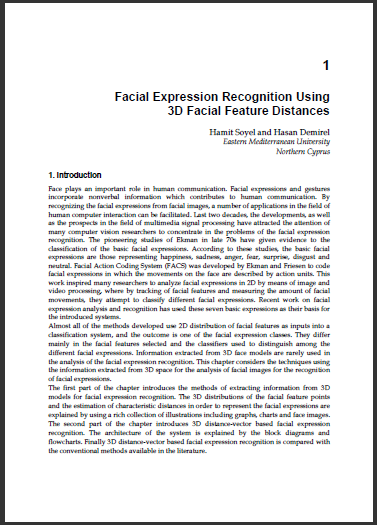
\includegraphics[width=0.5\textwidth]{./chapters/chapter08.png}
\caption{The opening page of a chapter in \textit{Affecting Computing}.}
\end{figure}

\solution To add the dot after the number can be done either using the key
\begin{verbatim}
\cxset{section numbering custom = \@arabic\c@section.,}
\end{verbatim}
or by using the pre-built key
\begin{verbatim}
\cxset{section number after=.}
\end{verbatim}

The author block including the institution are added as part of the chapter head styling command.

\example The subject of having articles together in a publication such as Proceedings and Journals is a recurring theme in many Academic fields. One of course if it is possible would have liked to use a standard Journal class and automatically produce this type of publication. There are a number of such classes at \href{http://ctan.org/tex-archive/macros/latex/required/amslatex/amscls/doc/instr-l.pdf}{ctan}

\solution If you are the editor with the task of assembling all these different articles consider using the \pkgname{confproc}. The package by Vincent Verfaille assembles the proceedings from the pdfs, using the 
\pkgname{pdfpages}, which is another great way to achieve this. A simpler way is to develop a specific style for
your Conference and let the participants use it while writing their papers. Only caveat they need to import the
body of the paper with \string\input\meta{article name}. As the \pkgname{phd} comes pre-packaged with
numerous packages the chance of someone using a package that the editor or the system needs to use it
is minimized. Indexing, bibliographies and the like might need to be taken care of and this is discussed in the relevant chapters. There are many options and peculiarities that might not be covered by the phd package so my suggestion is to try it on a few older papers first.

\example  Style-08 has to set the caption style to include for a period after the label number as shown in the Fig.~\ref{fig:eight02}. This can be achieved through key settings or a package.
\begin{figure}[ht]
\centering
\includegraphics[width=\textwidth]{./images/affective-computing.jpg}
\caption{Figures are centered, with the caption flush left and the \textit{Figure} label abbreviated to Fig. (with a stop). The section number also has the dot and follows the style of the sections.}
\label{fig:eight02}
\end{figure}

The figures numbers are reset at every chapter. Normally authors use the \pkgname{chngctr} to achieve such changes, which involves two modifications. Redefining whether or not the figure counter will be reset whenever the chapter/section counter is incremented; Redefining the "appearance" of the figure counter (\string\thefigure), i.e., removing (or adding) the chapter/section prefix.


The standard solution – which deals with modifications 1 and 2 mentioned above – is to use the \string\counterwithout and \string\counterwithin macros of the \texttt{chngcntr package}.\footnote{\protect\url{http://tex.stackexchange.com/questions/28333/continuous-v-per-chapter-section-numbering-of-figures-tables-and-other-docume}} 


\section{Tables}

The Tables follow the style for figures as far as captioning. They are all framed and although there is a genuine distain in the \latexe community for this type of style, I must admit that they are blending well with the style of this book. Another typographical tradition that has been broken in this book is that the table captions are placed below the table and not above.

\example
\begin{figure}[ht]
\centering
\includegraphics[width=\textwidth]{./images/affective-computing-tables.jpg}
\caption{Figures are centered, with the caption flush left and the \textit{Figure} label abbreviated to Fig. (with a stop). The section number also has the dot and follows the style of the sections.}
\label{fig:eight02}
\end{figure}


\begin{verbatim}
\cxset{table numbering=without}
\end{verbatim}

\setlength\extrarowheight{5pt}

\bgroup
\begin{table}[h]
\begin{tabularx}{\textwidth}{|c|c|c|X|}
\hline
Affective Movement & Mean & Standard Deviation &\RaggedRight Standard Error of the Mean\\
\hline
confident & (0.150,0.100,0.150) & (0.362,0.304,0.362)&(0.57,0.48,0.57)\\
\hline
\end{tabularx}
\caption{The table style of the book, with the caption below. You may need to increase the cell lengths.}
\end{table}
\egroup

The cell heights of the table have been increaded by 5pt, using,
\begin{verbatim}
\setlength\extrarowheight{5pt}
\end{verbatim}

\section{Front Matter}

The Front Matter includes a Title Page, Table of Contents and a Preface. Nothing special or exciting here with the exception of the Table of Contents which is a bit on the difficult side. 

\begin{figure}[ht]
\centering
\includegraphics[width=\textwidth]{./images/affecting-computing-contents.jpg}
\caption{Figures are centered, with the caption flush left and the \textit{Figure} label abbreviated to Fig. (with a stop). The section number also has the dot and follows the style of the sections.}
\label{fig:eight02}
\end{figure}

\section{Back Matter}



For the handling of the References there are numerous options and these are discussed under the Bibliography and References chapter.\footnote{\protect\url{http://tex.stackexchange.com/questions/87991/putting-bibliographies-at-the-end-of-each-chapter}} The referencing styles within paragraphs of text are author year in square brackets. I leave this to you.

\begin{figure}[ht]
\centering
\includegraphics[width=\textwidth]{./images/affective-computing-references.jpg}
\caption{Figures are centered, with the caption flush left and the \textit{Figure} label abbreviated to Fig. (with a stop). The section number also has the dot and follows the style of the sections.}
\label{fig:eight02}
\end{figure}

\parindent1em

There are no book divisions, such as an Index at the back of the book, but each chapter has its own references section, styled as a section. The occassional single Appendix appears at the end of a chapter, styled after sections and with no numbering marks.

\section{Concluding Remarks}

This template has a unique character and in my opinion deserves a bit better. Styling for algorithms, computer code additional floating sections and an index is not provided in the template and is left open for the user. It works well with the book class and with the KOMA classes. I have also given it an alias \emph{humanoid}\footnote{From one of the chapters in the book discussing the development of humanoids that can express emotions. The scientific field of human emotions and its applications both on the web as well as robotics is a vast topic. I did waste a lot of time reading the book rather than developing the style. } A minimal to use the template is shown below:

\section{Front Matter}
\begin{figure}[ht]
\centering
\includegraphics[width=\textwidth]{./images/facial-expression-1.jpg}
\caption{Figures are centered, with the caption flush left and the \textit{Figure} label abbreviated to Fig. (with a stop). The section number also has the dot and follows the style of the sections.}
\label{fig:eight02}
\end{figure}


\begin{verbatim}
\documentclass{book}
\usepackage{phd}
\cxset{humanoid}
\begin{document}
... contents
\end{document}
\end{verbatim}

If you do restyle it, please let me know with samples of the work.

\begin{key}{/phd/section align=center}{initial none}

\end{key}




%\cxset{author block=false}
\clearpage
\cxset{
 chapter name=none,
 numbering=arabic,
 number font-size=LARGE,
 number font-family=sffamily,
 number font-weight=mdseries,
 number before=,
 number dot=,
 number display=block,
 number float=left,
 number after={\vrule width2cm height0.4pt depth0pt\relax},
 number position=rightname,
 chapter font-family=sffamily,
 chapter font-weight=normalfont,
 chapter font-size=Large,
 chapter before={\vspace*{10pt}\par},
 chapter after={},
 chapter color={black!90},
 number color= black!90,
 title beforeskip=,
%title afterskip={\vspace*{50pt}\par},
 title margin bottom=40pt,
 title before=,
 title after=,
 title font-family=sffamily,
 title font-color= black,
 title font-weight=normalfont,
 title font-size=LARGE,
 chapter title align=none,
chapter title text-align=left,
chapter title width=\textwidth,
 title margin top=0pt,
 section numbering=none,
 section font-weight=normalfont,
 section indent=0pt,
 section align=centering,
 }
 \renewsection
\chapter{Preparing for Trial}

Template number nine, is from a book about a the Rivonia Trial. The template is easy to set up and is has a simple but effective design, which I think is very appropriate for a journalistic type of book. 
\medskip
\begin{figure}[ht]
\centering
\hspace*{-.1\textwidth}{\color{thegray}\fbox{\includegraphics[width=1.2\textwidth]{mandela-01}}}
\end{figure}

When South Africa's apartheid government charged Nelson Mandela with planning its overthrow in 1963, most observers feared that he would be sentenced to death. But the support he and his fellow activists in the African National Congress received during his trial not only saved his life, but also enabled him to save his country. In Saving Nelson Mandela, South African law expert Kenneth S. Broun recreates the trial--called the ``Rivonia" Trial after the Johannesburg suburb where police seized Mandela. Based upon interviews with many of the case's primary figures and portions of the trial transcript, Broun situates readers inside the courtroom at the imposing Palace of Justice in Pretoria. Here, the trial unfolds through a dramatic narrative that captures the courage of the accused and their defense team, as well as the personal prejudices that colored the entire trial. The Rivonia trial had no jury and only a superficial aura of due process, combined with heavy security that symbolized the apartheid government's system of repression. 

Broun shows how outstanding advocacy, combined with widespread public support, in fact backfired on apartheid leaders, who sealed their own fate. Despite his 27-year incarceration, Mandela's ultimate release helped move his country from the racial tyranny of apartheid toward democracy. As documented in this inspirational book, the Rivonia trial was a critical milestone that helped chart the end of Apartheid and the future of a new South Africa.

``Kenneth Broun does justice indeed to one of the most celebrated political trials of the 20th century...the result is not only a gripping story but a work of profound scholarship, sensitivity, and empathy." --Mark Gevisser, author of A Legacy of Liberation 

``Part history, part sociology, part engrossing legal drama, this important book recounts a seminal moment in South Africa's history." --Penelope Andrews, City University of New York School of Law

Many things are going wrong in South Africa, but it would have been worse if it was not for Mandela.  

To use the template simply load the \pkgname{phd} package and |style09| or |rivonia|. Adjust spacing fonts and geometry to your liking:

\begin{verbatim}
\documentclass{book}
\usepackage{phd}
\phdusetemplate{style09}
\cxset{chapter opening=anywhere}
\begin{document}
\chapter{Arrests and Escapes}
\end{document}
\end{verbatim}

\cxset{chapter opening=anywhere}

\chapter{Arrests and Escapes}

\lorem

\section{Adjusting the Rule}

You might want to fiddle with the rule settings, as well as the section settings. I prefer the sections centered and not numbered.

\thispagestyle{headings}









%<<<<<<< HEAD
%%%%%%%%%%%%%%%%%%%%%%%%%%%%%%%%%%%%%%%%%%%
%%%%%%  STYLE 10
%%%%%%%%%%%%%%%%%%%%%%%%%%%%%%%%%%%%%%%%%%%

\cxset{
 name=CHAPTER,
 numbering=WORDS,
 number font-size=\huge,
 number font-family=\sffamily,
 number font-weight=\bfseries,
 number before=,
 number dot=,
 number after=\hspace{1em},
 number position=rightname,
 chapter font-family=\sffamily,
 chapter font-weight=\bfseries,
 chapter font-size=\huge,
 chapter before={\vspace*{0.4\textheight}\hfill},
 chapter after={\hfill\hfill\vskip0pt\thinrule\par},
 chapter color={black!90},
 number color=\color{black!90},
 title beforeskip={\vspace*{30pt}},
 title afterskip={\vspace*{30pt}\par},
 title before={\hfill},
 title after={\hfill\hfill},
 title font-family=\sffamily,
 title font-color=\color{black!90},
 title font-weight=\bfseries,
 title font-size=\huge,
 section font-size=\LARGE,
 section font-weight=\normalfont,
 section font-family=\sffamily,
 section align=,
 section numbering=none,
 section indent=-1em,
 section align=\centering,
 section beforeskip=20pt,
 section afterskip=10pt,
 section spaceout=soul,
 section font-shape=,
}

 %set the sectioning commands


\renewsection

\chapter{INTRODUCTION TO STYLE TEN}

\section{Basic Description:}
This chapter style has the unique characteristic that the chapter number is spelled out, rather than being in arabic numerals. The setting for this is the option \lstinline{numeric=WORDS}. Use either a capital for uppercase or \lstinline{numeric=words} for lowercase number labels.

\medskip
\begin{figure}[ht]
\centering
\includegraphics[width=0.6\textwidth]{./chapters/chapter10}
\end{figure}

\lipsum[1]
=======
%%%%%%%%%%%%%%%%%%%%%%%%%%%%%%%%%%%%%%%%%%%
%%%%%%  STYLE 10
%%%%%%%%%%%%%%%%%%%%%%%%%%%%%%%%%%%%%%%%%%%

\cxset{
 name=CHAPTER,
 numbering=WORDS,
 number font-size=\huge,
 number font-family=\sffamily,
 number font-weight=\bfseries,
 number before=,
 number dot=,
 number after=\hspace{1em},
 number position=rightname,
 chapter font-family=\sffamily,
 chapter font-weight=\bfseries,
 chapter font-size=\huge,
 chapter before={\vspace*{0.4\textheight}\hfill},
 chapter after={\hfill\hfill\vskip0pt\thinrule\par},
 chapter color={black!90},
 number color=\color{black!90},
 title beforeskip={\vspace*{30pt}},
 title afterskip={\vspace*{30pt}\par},
 title before={\hfill},
 title after={\hfill\hfill},
 title font-family=\sffamily,
 title font-color=\color{black!90},
 title font-weight=\bfseries,
 title font-size=\huge,
 section font-size=\LARGE,
 section font-weight=\normalfont,
 section font-family=\sffamily,
 section align=,
 section numbering=none,
 section indent=-1em,
 section align=\centering,
 section beforeskip=20pt,
 section afterskip=10pt,
 section spaceout=soul,
 section font-shape=,
}

 %set the sectioning commands


\renewsection

\chapter{INTRODUCTION TO STYLE TEN}

\section{Basic Description:}
This chapter style has the unique characteristic that the chapter number is spelled out, rather than being in arabic numerals. The setting for this is the option \lstinline{numeric=WORDS}. Use either a capital for uppercase or \lstinline{numeric=words} for lowercase number labels.

\medskip
\begin{figure}[ht]
\centering
\includegraphics[width=0.6\textwidth]{./chapters/chapter10}
\end{figure}

\lipsum[1]
>>>>>>> merged

%\cxset{style11/.style={
 chapter opening=any,
 name=Chapter,
 numbering=arabic,
 number font-size=LARGE,
 number font-family=rmfamily,
 number font-weight=bfseries,
 number before=,
 number dot=,
 number after=,
 number before=\kern0.5em,
 number display=inline,
 number float=center,
 chapter display=block,
 chapter float=center,
 chapter font-family=rmfamily,
 chapter font-weight=bfseries,
 chapter font-size=LARGE,
 chapter before=,
 chapter after=,
 chapter color=black!90,
 chapter spaceout=none,
 chapter border-width=0pt,
 chapter border-style=none,
 number color=black!90,
 title beforeskip=,
 title afterskip=,
 title before=,
 title after=,
 title font-family=rmfamily,
 title font-color=black!90,
 title font-weight=bfseries,
 title font-size=LARGE,
 chapter title width=\textwidth,
 chapter title align=centering,
 section afterindent=true,
 section align=left,
 section numbering=arabic,
 section numbering prefix=\thechapter.,
 section numbering suffix=\space,
 section indent=0pt,
 section font-family=rmfamily,
 }}
\renewsection\renewsubsection

\cxset{style11}
\chapter{\textit{Elements} II and Babylonian Metric Algebra, Introduction to Style Eleven}

The origins of Greek Mathematics, according to the Greeks is Egypt and according to J\"oran Friberg is Babylonia. This template is based on Friberg's book \emph{Amazing Traces of a Babylonian Origin in Greek Mathematics}. The book was published by World Scientific in 2007. The book size is $5.97\times8.88$ inches and uses a variety of fonts, with the main document font in Times. 

\medskip
\begin{figure}[ht]
\centering
\fbox{\includegraphics[width=0.65\textwidth]{./chapters/chapter11.png}}
\end{figure}
\lipsum[1]

\section{Indentation}

The book follows swedish traditional typography with the paragraphs following subheadings indented. This is achieved in the template using:

\begin{verbatim}
\cxset{section afterindent=true}
\end{verbatim}

\section{Images}
\indent Images and their captions follow a \latexe style and I am sure the book must have been styled using a \latexe xml clone as the book's pdf was produced with iText\footnote{\url{http://itextpdf.com/}}.

\begin{figure}[ht]
\centering
\includegraphics[width=0.8\textwidth]{greekmaths}
\caption{Extract from the \textit{Amazing Traces of Babylonian Influence in Greek Mathematics.} Note the styling of the caption.}
\end{figure}

\testsections

% reset for following chapters
\cxset{section afterindent=false}


%\parindent0pt
\makeatletter
\cxset{style12/.style={%
 chapter name=,
 chapter toc=true,
 chapter numbering=arabic,
 number font-size=HUGE,
 number font-family=rmfamily,
 number font-weight=bfseries,
 number before=,
 number dot=,
 number color= gray,
 number after=,
 number position=rightname,
 number float=left,
 number display=block,
 chapter font-family=sffamily,
 chapter font-weight=normalfont,
 chapter font-size=huge,
 chapter before=,
 chapter after=,
 chapter color={black!90},
 title beforeskip={\vspace*{0pt}},
 title afterskip={\vspace*{50pt}\par},
 title before=,
 title after={\par\vspace{20pt}\rule{\textwidth}{4pt}},
 title font-family=sffamily,
 title font-color=black!90,
 title font-weight=bfseries,
 title font-size=Huge,
 title font-shape=normal,
 title spaceout=none,
 chapter title width=.8\textwidth,
 chapter title align=left,
 chapter title text-align =left,
}}
\makeatother

\cxset{style12}
\chapter{Why Have They Become Mainstream so Quickly? }
\label{ch:style12}
This is a variation of Style 7, with only the lettering and the rule are thicker. In my opinion it looks better with a bit of color, so I have used a purple color with a gray.

\medskip
\begin{figure}[ht]
\centering
\includegraphics[width=0.35\textwidth]{./chapters/chapter12.png}
\caption{Style 12 sample from the book.}
\end{figure}
\lipsum[1]


%\makeatletter

\cxset{plain sections/.style={
 chapter opening = right, 
 chapter name = CHAPTER,
 chapter toc = true,
 chapter color= thelightgray,
 chapter numbering = arabic,
 chapter font-family= sffamily,
 chapter font-weight= bold,
 chapter font-size= LARGE,
 chapter before={\vspace*{20pt}\par\hfill\hfill},
 chapter after={\vskip0pt\par},
 chapter spaceout = soul,
 number font-size= Large,
 number font-family= rmfamily,
 number font-weight= mdseries,
 number color=thegray,
 number before=\vspace*{5pt}\hfill\hfill,
 number dot=,
 number after={\hspace*{7pt}\par},
 title beforeskip={\vspace*{10pt}},
 title afterskip={\vspace*{50pt}\par},
 chapter title align=none,
 title before=\par\hfill\hfill..,
 title after=\par,
 title font-family=\sffamily,
 title font-color= teal,
 title font-weight=\bfseries,
 title font-family=\sffamily,
 title font-size= Large,
 title font-shape= upshape,
 title spaceout= none,
 title beforeskip={\vspace*{10pt}},
 title afterskip={\vspace*{50pt}\par},
 title before={\hfill\hfill\raggedleft},
%
% numbers
% number font-family=\sffamily,
% number font-weight=\bfseries,
 number color=thelightgray,
 number before=\par\vspace*{5pt}\hfill\hfill,
 number dot=.,
 number after={\hspace*{7pt}\par},
 number position=rightname,
 section color= thered,     
 section beforeskip=15pt,
 section afterskip=15pt,
 section indent=0pt,
 section font-family= sffamily,
 section font-size= LARGE,
 section font-weight= bfseries,
 section font-shape=,
 section align= centering,
 section numbering prefix =,%use \thechapter. for books or add as option
 section numbering= arabic,
 section spaceout=none,
 section number after=,
section afterindent=false,
 subsection color= thered,
 section numbering suffix=,
       subsection beforeskip=10pt,
       subsection afterskip=10pt,
       subsection indent=0pt,
       subsection font-family= sffamily,
       subsection font-size= Large,
       subsection font-weight= bold,
       subsection font-shape= upshape,
       subsection align= centering,
       subsection numbering prefix=\thesection.,%\S\hairsp,%add . 
       subsection numbering custom =\@arabic\c@subsection,% \two@digits{\@arabic\c@subsection},%
       subsubsection color= gray,
       subsubsection beforeskip=5pt plus3pt minus 2pt,
       subsubsection afterskip=5pt,
       subsubsection indent=0pt,
       subsubsection font-family= rmfamily,
       subsubsection font-size= \large,  %normalfont gives problems
       subsubsection font-weight= bold,
       subsubsection font-shape= itshape,
       subsubsection align= centering,
       subsubsection numbering prefix =\thesubsection.\@arabic\c@subsubsection,
       subsubsection numbering custom =, %\two@digits{\@arabic\c@subsubsection},
       subsubsection number after =, 
%
       paragraph color= thegrey,
       paragraph beforeskip=,
       paragraph afterskip=-0.5em,
       paragraph indent=0pt,
       paragraph font-family= rmfamily,
       paragraph font-size= large,
       paragraph font-weight= bfseries,
       paragraph font-shape=,
       paragraph align= centering,
       paragraph number after = 0pt,
       paragraph numbering=numeric,
       subparagraph color= thered,
       subparagraph beforeskip=0pt,
       subparagraph afterskip=-.5em,
       subparagraph indent=0pt,
       subparagraph font-family= sffamily,
       subparagraph font-size= large,
       subparagraph font-weight= normalfont,
       subparagraph font-shape= slshape,
       subparagraph align= RaggedRight,
       subparagraph number after =, % can affect all needs checking
       %subsubsection numbering prefix=\S\hairsp\thesection,%add . here if need be
       subparagraph numbering=none,
     }
}
\cxset{plain sections}

\cxset{companion/.style={
 name=,
 chapter spaceout =none,
 numbering=arabic,
 number font-size=huge,
 number font-family=rmfamily,
 number font-weight=bfseries,
 number color=black!50,
 number before=,
 number dot=,
 number after=,
 number display=block,
 number float=center,
 number position=rightname,
 chapter font-family= sffamily,
 chapter font-weight= bold,
 chapter font-size= LARGE,
 chapter before=\hfill,
 chapter color= black!50,
 title beforeskip={\vspace*{10pt}},
 title afterskip={\vspace*{50pt}\par},
 title before=\hfill,
 chapter rule color=spot!50,
 title after=\hfill\hfill,
 title font-family= rmfamily,
 title font-color= black,
 title font-weight= bfseries,
 title font-size= huge,
 chapter title width=\textwidth,
 chapter title align=centering,
 chapter title text-align=center,
 % section styling
 section align= centering,
 section numbering= none,
 section indent=0pt,
 section beforeskip=-10pt,
 section afterskip= 10pt,
 section color= black,
 section font-size=Large,
 section font-weight=bold,
 section font-family=rmfamily,
 section number after=,
 subsection align=centering,
 subsection beforeskip=10pt,
 subsection indent=0pt,
 subsection afterskip=0.5\baselineskip,
 subsection font-family=\rmfamily,
 subsection font-weight= bfseries,
 subsection font-shape= \itshape,
 subsection color = black,
 subsection font-size= normalsize,
 subsection numbering=none,
 subparagraph number after=,
 subsubsection align=,
 subsubsection color=black,
 author block=true,
author block format=\vspace{10pt},
 author names={\aegean DAVID KEYT},
}
}
\makeatother

\cxset{companion}



\lorem

\parindent=1em
\pagestyle{centerheadings}
\captionsetup{labelfont=bf, textfont=bf, justification=centering, width=0.8\textwidth, labelsep=period}
%\thispagestyle{myheadings}

\cxset{caption setup/.code=\captionsetup{#1} }
\cxset{caption setup = {labelfont=bf, textfont=bf, justification=centering, width=0.8\textwidth, labelsep=period} }

\chapter{Aristotle’s Political Philosophy}


But while book production is increasing and books now may seem with no end, they do have a more definite beginning, as the ancient preacher also may have known. William M. Schniedewind’s book, \emph{How the Bible Became a Book}, traces the history of the Hebrew Bible and provides archaeological evidence and insights from linguistic anthropology,
that point to the earlier era of the late Iron Age (eighth
though sixth centuries b.c.e.) as the formative period for the writing
of biblical literature and not in the Persian and Hellinistic periods (the fifth through second centuries \textsc{b.c.e} 
\citep{schniedewind2005}. It is a book that I have enjoyed and can recommend it to the general reader as well as the Biblical Studies scholar. The book  provides rich insight into why these
texts came to have authority as Scripture and explores why ancient
Israel, an oral culture, began to write literature. It describes an emerging
literate society in ancient Israel that challenges the assertion that
literacy first arose in Greece during the fifth century \textsc{b.c.e.} It has a simple and serious
typography appropriate for its subject and I have included it in this collection of templates for its many additional textual requirements, such as the quotations from biblical texts.

I have based most of the templates and themes provided on books that I own and have read. Michael Harkins \citep{harkins2013} investigated how to quantify the expertness of type designers and concluded that this is not possible. My own interest is to investigate ther emic and etic of Book Designers and to apply it to the automated production of books. So hopefuly by the simple mimicking of current book designs I am hoping that some theoretical knowledge will emerge for such definitions. To date little has been published that attempts to account for processes involved in the designing of typefaces and books, although many books on graphic design provide ample information on subproblems of the process. Some of the findings are easier to quantify than others, but the
general process is still difficult to define. For example if one has to deal with figures some rules can be deduced for sizing and captioning. Others relating to heading sizes can also be quantified and programmed in an automated system. Others such as to when to include rules or special designs in a chapter heading are difficult to assess as to what makes them attractive to the reader and the process which the Book Designer used to produce such final designs. The provision of the template mechanism, provides a technique for implementing such layouts, but is no way claiming that Book Design can be automated. I have chosen this particular book and template to outline the mehod as the book is primarily text orientation with very few figures and simple headings designs. Such designs are very easy to implement using the approach provided by this package.  Michael Harkins discusses etic and
emic with regard to the outside observer's knowledge of type design versus the designer’s internal knowledge or
“expertness”.  Knuth certainly applied similar techniques in understanding and codifying the compositor’s profession with his expert design of the \tex typesetting engine. However, the broader subject of book design was delegated to the user and the output routine. 

\section{Using the Template}

The template can be used easily by loading the style file.

\begin{verbatim}
\documentclass{book}
\usepackage{phd}
\cxusetemplate{style13}
\begin{document}
...
\end{document}
\end{verbatim}

The style file does not need to be loaded in the preamble, although I recommend it. It can be loaded at
any stage in the document.

All the document styles provided with the \pkgname{phd} have not been optimized in terms of font usage and spacing, as they are so easy to modify. The reason for this was to make them widely available in a format that
is widely available. The spacing decision was to allow this document to be produced with some form of style.

After we first analyze and determine the sectioning of the book we start from the chapter sectioning. You can use the default template to start with and modify only the settings that are affected. An extract from the book is shown in figure~ref{fig:biblical}. We first set the keys

\begin{figure}[htb]
\includegraphics[width=\textwidth]{./images/bible-book.jpg}
\caption{The first chapter opening of \textit{How the Bible Became a Book}, published by the Cambridge University Press \protect\citep{schniedewind2005}.}
\label{fig:biblical}
\end{figure}

\section{Textual Elements}
\subsection{Quoting and numbering lines}

The text quotes extensively from the Jewish Bible as well as Temple Scrolls, using a style normally found in biblical books and journals.
\medskip

{\normalsize

\noindent\underline{Deuteronomy 17:14}. When you have come into the land that YHWH your God is
giving you,12 and have taken possession of it and settled in it, and you say, “I will set
a king over me, like all the nations that are around me,” \underline{15} you may indeed appoint
a king whom YHWH your God will choose. From one of your brethren you shall set
a king over you\ldots.
\medskip

\noindent\underline{Temple Scroll (11QT$^{\text{a}}$) 56:12}.  When you have come into the land that I am giving
you, and have taken possession and settled in it, \ul{13} and you say, “I will set a king
over me, like all the nations that are around me,” \ul{14} you may indeed set a king over
yourselves – one whom I will choose. From one of your brethren you shall set a king
over you\ldots.}
\medskip

Other quotes from the Bible take the form:
\medskip

The first mention of this
book follows the little poem in Joshua 10:12–13 recounting the day
the sun stood still:
\begin{smallverbatim}
On the day when YHWH gave the Amorites over to the Israelites,
Joshua spoke to YHWH; and he said in the sight of Israel,
“Sun, stand still at Gibeon,
and Moon, in the valley of Aijalon.”
And the sun stood still, and the moon stopped,
until the nation took vengeance on their enemies.
Is this not written in the Book of Jashar? 
The sun stopped in mid-heaven, and did
not hurry to set for about a whole day.
\end{smallverbatim}

\begin{macro}{\smallverbatim}
\begin{macro}{\smallverbatimfont}
The above is typeset using a \cmd{\smallverbatim} environment, but with the font defined as a \cmd{\smallverbatimfont}  and typeset in smaller type. 
\end{macro}
\end{macro}

\section{Figures}

Figures are floated to top or bottom of the page. They are styled centered and the caption is constrained within the figure.

\captionsetup{labelfont=bf, textfont=bf, justification=centering}

\begin{figure}[htbp]
\centering
\includegraphics[width=.8\textwidth]{./images/bible-book-figures.jpg}
\caption{\smallish Some figure pages. Most have citations and figure credits. The caption is centered within the width of the image}
\end{figure}


\subsection{Coding for landscape figures}

A landscape figure is illustrated in Figure~\ref{sidecantor}. Note that you must add the label information twice (in this case, \verb"sidecantor"). Here is the source code:
\begin{verbatim}
  \begin{sidewaysfigure}{sidecantor}
    %  note that the square brace option below is only required
    %  if you intend to produce a list of illustrations
    \caption[Landscape figure]{A~Cantor repeller.}
    \label{sidecantor}
    \includegraphics[scale=0.85]{./images/nudes.jpg}
  \end{sidewaysfigure}
\end{verbatim}
  \begin{sidewaysfigure}%{sidecantor}
    %  note that the square brace option below is only required
    %  if you intend to produce a list of illustrations
    \caption[Landscape figure]{A~Cantor repeller.}
    \label{sidecantor}
    \includegraphics[scale=0.85]{./images/yaleartschool.png}
  \end{sidewaysfigure}

\subsection{Coding for landscape tables}

A landscape table is illustrated in Table~\ref{warefeatures}. Note that you must add the label information twice (in this case, \verb"warefeatures"). Also, you only need to use the minipage environment \verb"\begin{minipage}...\end{minipage}" if your table contains a footnote. Here is the source code:
\begin{smallverbatim}
  \begin{sidewaystable}{warefeatures}
    \caption[Landscape table]{Grooved ware and beaker features,
      their finds and radiocarbon dates. For a breakdown of the
      pottery assemblages see Tables~I and~III; for the flints see
      Tables~II and~IV; for the animal bones see Table~V.}
    \label{warefeatures}
    \begin{minipage}{440pt}% use only if you have a table footnote
    %\smallertablesize % uncomment if your table does not fit the depth
    \begin{tabular}{@{}lcccllccc@{}}
    \hline\hline
    Context\footnote{If you are using footnotes, you must be in a minipage
      environment.}
    & Length & Breadth/ & Depth & Profile & Pottery & Flint
    & Animal & C14 Dates\\
    & & Diameter & & & & & Bones\\[5.5pt]
    & m & m & m\\
    \hline\\[-5.5pt]
    \multicolumn{9}{@{}l}{\textbf{Grooved Ware}}\\
    784 & -- & 0.9$\phantom{0}$ &0.18  & Sloping U & P1     & $\times$46
        & $\phantom{0}$$\times$8  & 2150 $\pm$100\,\textsc{bc}\\
    785 & -- & 1.00             &0.12  & Sloping U & P2--4  & $\times$23
        & $\times$21 & --\\
    962 & -- & 1.37             &0.20  & Sloping U & P5--6  & $\times$48
        & $\times$57 &  1990 $\pm$80\,\textsc{bc} (Layer 4)\\
    & & & & & & & & 1870 $\pm$90\,\textsc{bc} (Layer 1)\\
    983 & 0.83     & 0.73       &0.25  & Stepped U & --     & $\times$18
    & $\phantom{0}$$\times$8  & --\\[\baselineskip]
    \multicolumn{9}{@{}l}{\textbf{Beaker}}\\
    552 & -- & 0.68             & 0.12 & Saucer    & P7--14 & --
        &-- &--\\
    790 & -- & 0.60             & 0.25 & U         & P15    & $\times$12
        & --   &--\\
    794 & 2.89                  & 0.75 & 0.25      & Irreg. & P16
        & $\phantom{0}$$\times$3  &-- &--\\
    \hline\hline
    \end{tabular}
    \end{minipage}
  \end{sidewaystable}
\end{smallverbatim}

% Sideways table
  \begin{sidewaystable}%{warefeatures}
   \captionsetup{type=table, justification=raggedright, width=6cm,margin=0cm, textfont=small}
    \caption[Landscape table]{Grooved ware and beaker features,
      their finds and radiocarbon dates.\\ For a breakdown of the
      pottery assemblages\\ see Tables~I and~III; for the flints see
      Tables~II and~IV; for the animal bones see Table~V.}
      
    \label{warefeatures}
    \begin{minipage}{440pt}% use only if you have a table footnote
    %\smallertablesize % uncomment if your table does not fit the depth
    \begin{tabular}{@{}lcccllccc@{}}
    \hline\hline
    Context\footnote{If you are using footnotes, you must be in a minipage
      environment.}
    & Length & Breadth/ & Depth & Profile & Pottery & Flint
    & Animal & C14 Dates\\
    & & Diameter & & & & & Bones\\[5.5pt]
    & m & m & m\\
    \hline\\[-5.5pt]
    \multicolumn{9}{@{}l}{\textbf{Grooved Ware}}\\
    784 & -- & 0.9$\phantom{0}$ &0.18  & Sloping U & P1     & $\times$46
        & $\phantom{0}$$\times$8  & 2150 $\pm$100\,\textsc{bc}\\
    785 & -- & 1.00             &0.12  & Sloping U & P2--4  & $\times$23
        & $\times$21 & --\\
    962 & -- & 1.37             &0.20  & Sloping U & P5--6  & $\times$48
        & $\times$57 &  1990 $\pm$80\,\textsc{bc} (Layer 4)\\
    & & & & & & & & 1870 $\pm$90\,\textsc{bc} (Layer 1)\\
    983 & 0.83     & 0.73       &0.25  & Stepped U & --     & $\times$18
    & $\phantom{0}$$\times$8  & --\\[\baselineskip]
    \multicolumn{9}{@{}l}{\textbf{Beaker}}\\
    552 & -- & 0.68             & 0.12 & Saucer    & P7--14 & --
        &-- &--\\
    790 & -- & 0.60             & 0.25 & U         & P15    & $\times$12
        & --   &--\\
    794 & 2.89                  & 0.75 & 0.25      & Irreg. & P16
        & $\phantom{0}$$\times$3  &-- &--\\
    \hline\hline
    \end{tabular}
    \end{minipage}
  \end{sidewaystable}

\cxset{author block=false}

\restoregeometry





 % CHECK FOR ERRORS
%\cxset{%
 chapter opening=any,
 name=Chapter,
 numbering=arabic,
 number font-size=HHUGE,
 number font-family=rmfamily,
 number font-weight=bfseries,
 number before=,
 number dot=,
 number after=,
 number position= rightname,
 number display=block,
 number float=right,
 chapter display=block,
 chapter float=right,
 chapter font-family=\sffamily,
 chapter font-size=\Large,
 chapter before={\offinterlineskip\hbox{\vrule height2pt width\textwidth}\vskip3.5pt}\hfill,
 chapter after=\vskip3.5pt,
 chapter color=black!90,
 number color=black!90,
 chapter title width={0.5\textwidth},
 title margin-left=0pt,
 chapter title align=right,
 chapter title text-align=raggedleft,
 chapter margin top=0pt,
 chapter margin-left=0pt,
 title margin top=0pt,
 title margin bottom=10pt,
 title before={},
 title after={},
 title font-family=sffamily,
 title font-color=black!90,
 title font-weight=bfseries,
 title font-size=LARGE,
 section numbering prefix=\thechapter.,
 section color=black,
 subsection color=black}
 
\chapter{Review of Basic Fluid Mechanics Concepts}
\thispagestyle{headings}

This book is $5.51\times9.06$ inches and was produced according with the soft copy I have with Acrobat Distiller 5.0 (Windows). It uses a variety of fonts Arial, Century Schoolbook and Helvetica, Times Roman, MathematicalPi-One.
\medskip
\begin{figure}[ht]
\centering
\fbox{%
\includegraphics[width=0.45\textwidth]{./chapters/chapter14}
\includegraphics[width=0.45\textwidth]{./chapters/chapter14a.png}}
\end{figure}
\lipsum[2]

\section{Images}

\begin{figure}[ht]
\centering
\includegraphics[width=0.8\textwidth]{biofluids}
\end{figure}
\lipsum[2]

\lipsum[1]
\section{Examples}
Both full page ad well as block examples exist, these are all in boxes and they are numbered either with subsection counters in a fashion that is continuous from the text. 
\begin{figure}[ht]
\centering
\includegraphics[width=0.8\textwidth]{biofluids-1}
\end{figure}
\lipsum[2-4]

\begin{figure}[!b]
\begin{scriptexample}{This is a test}{}
\subsection{Clinical feature: polycythemia}

Polycythemia refers to a condition in which there is an increase in hemoglobin
above 17.5 g/dL in adult males or above 15.5 g/dL in females
(Hoffbrand and Pettit, 1984). There is usually an icrease in the number of
red blood cells above 6 - 1012 $L{^1}$ in males and 5.5 - 1012 $L^{-1}$ in females.
That is, a sufferer from this condition has a much higher blood viscosity due
to this elevated red blood cell count.
\end{scriptexample}
\end{figure}

Our boxes with the \pkgname{tcolorbox} are more than adequate for the job. The color settings can be changed via normal tcolorbox key settings that I have linked to the phd package keys.

The boxes can be also turned into floating boxes and to force them either to be on a full page or at the bottom in order for them to make a better impact in the layout. Key settings for setting the color of the boxes are provided
as well as a special environment.

\begin{verbatim}
\cxset{example box color=thegray}
\end{verbatim}

These example or sideboxes can easily be modified and you may have to provide your own, if you want anything particularly fancy. See the tcolorbox manual for many setting, but please do not use rounded boxes. 
%\end{document}
%%%%%%%%%%%%%%%%%%%%%%%%%%%%%%%%%%%%%%%%%%%%
%%%%%%  STYLE 15
%%%%%%%%%%%%%%%%%%%%%%%%%%%%%%%%%%%%%%%%%%%
\newgeometry{left=2cm,right=7cm, marginparsep=15pt, marginparwidth=4.2cm,top=2cm}
\cxset{
 name={},
 numbering=none,
 number font-size=\LARGE,
 number font-family=\rmfamily,
 number font-weight=\bfseries,
 number before=,
 number dot=,
 number after=,
 number position=rightname,
 chapter font-family=\sffamily,
 chapter font-weight=\normalfont,
 chapter font-size=\Large,
 chapter before={},
 chapter after={},
 chapter color={black!90},
 number color=\color{purple},
 title beforeskip={},
 title afterskip={\vspace*{50pt}\par},
 title before={},
 title after={},
 title font-family=\rmfamily,
 title font-color=\color{black!80},
 title font-weight=\normalfont,
 title font-size=\Huge,
 title font-shape=\itshape,
 chapter opening=any,
 watermark text=SAMPLE PAGE,
 header style=samplepage}


\chapter{Introduction to Style Fifteen}

\parindent1em
\def\thefigure{\arabic{chapter}.\arabic{figure}}
\lorem\par

\marginpar{%
 {\centering
 \includegraphics[width=4.2cm]{./chapters/chapter15}\vskip5pt\par}
 {\footnotesize\lorem}
}
\marginpar{%
{\centering
\includegraphics[width=4.2cm]{./chapters/chapter15}\par}
 { \captionof{figure}{\footnotesize\lorem}}
}
This is another marginpar of the same size.

\lorem

\lipsum
\marginpar{%
{\centering
\includegraphics[width=4.2cm]{./chapters/chapter15}\par}
 { \captionof{figure}{\footnotesize\lorem}}
}
%%%% END STYLE %%%%%%%%%%%%%%%%%%%%%%%%%%%%%%%%%

%
\newgeometry{left=7.5cm,right=2cm, marginparsep=15pt, marginparwidth=4.2cm,top=2cm}
%%%%%%%%%%%%%%%%%%%%%%%%%%%%%%%%%%%%%%%%%%%
%%%%%%  STYLE 16
%%%%%%%%%%%%%%%%%%%%%%%%%%%%%%%%%%%%%%%%%%%


\cxset{style16/.style={
 chapter opening=anywhere,
 name={},
 numbering=arabic,
 number color=\color{thegray},
 number font-size=\HHUGE,
 number font-family=\rmfamily,
 number font-weight=\bfseries,
 number before=\leftskip-4cm\vbox to 0cm\bgroup\vspace*{5cm},
 number after=\egroup\vskip0pt\par,
 number dot=,
 number position=leftname,
 chapter font-family=\sffamily,
 chapter font-weight=\normalfont,
 chapter font-size=\Large,
 chapter before={},
 chapter after={\begin{picture}(0,0)
                          \put(-50pt,\dimexpr-\textheight+\footskip+20pt\relax){\parbox{\marginparwidth}{\textbf{Napoleon}\par\lorem}}%
                        \end{picture}},
 chapter color={black!90},
 title beforeskip={\par\hspace*{4cm}\thinrule\vskip0pt\hspace*{4cm}\vbox\bgroup},
 title afterskip={\vspace*{50pt}\par\egroup},
 title before={},
 title after=,
 title font-color=\color{black!80},
 title font-weight=\normalfont,
 title font-family=\rmfamily,
 title font-shape=\upshape,
 title font-size=\HUGE,
 header style=empty,
 subsection numbering=none,
 subsection color=teal,
 subsection align=\color{teal},
 header style=empty,
 }}

\renewsubsection

%%%% VERSO NAPOLEON %%%%%%%%%%%
% We define a macro to set the page dimensions to full.
% We also require the parindent to be set to 0pt and to restore it afterwards.
\def\fullpageimage{%
       \vspace*{-2.5cm}
        \parindent0pt
       \hspace*{-2cm}\includegraphics[width=\paperwidth]{napoleon}%

}


\cleardoublepage
\fullpageimage

\cxset{style16}
\chapter{Victorian England:\\ Introduction 16}
\label{style16}
This design from a Social Sciences book had to be set into two vboxes and negative skips allowed to line
up the numbers. Once I am totally happy with it, I will add parameter adjustments, as well as a bit of automation of length calculations.
\thispagestyle{empty}

\medskip

\begin{figure}[ht]
\centering
\includegraphics[width=0.35\textwidth]{./chapters/chapter16}
\end{figure}
\lipsum[2]

\cxset{geometry marginparsep/.code=\setlength\marginparsep{#1},
          geometry marginparwidth/.code=\setlength{\marginparwidth}{#1}}

\section{Technical notes}

This design looks simple but takes a bit of effort to achieve it, especially due to the tendency of LaTeX and the TeX engine to make decisions for you. Firstly we cannot reset the page geometry between the image and the chapter, as this will either result in unpredictable behaviour or if you use the \cs{newgeometry} macro, it will for certain leave a blank page in between.

\begin{description}
\item [image sizing] The image is set at \textbf{width=paperwidth}. This can vary depending on the page geometry and the image aspect ratio. In general you may need to ensure that your image has the same aspect ratio as the page to avoid problems with placement and the generation of extra blank pages.
\item [image caption] The image caption is placed using the picture environment, so that it can be typeset absolutely, feel free to use TikZ for the same purpose. We also use Heiko Oberdiek's the \pkg{picture} package to make calculations easier by specifying actual dimensions and not needing to strip the point.
\end{description}

% Best to always restore geometry after you have changed it.

\restoregeometry


%%%%%%%%%%%%%%%%%%%%%%%%%%%%%%%%%%%%%%%%%%%%
%%%%%%  STYLE 17
%%%%%%%%%%%%%%%%%%%%%%%%%%%%%%%%%%%%%%%%%%%
\newgeometry{left=7cm,right=2cm, marginparsep=15pt, marginparwidth=4.2cm,top=2cm,%
reversemarginpar}
\cxset{style17/.style={
 name={},
 numbering=arabic,
 number font-size=\huge,
 number font-family=\sffamily,
 number font-weight=\bfseries,
 number before=,
 number dot=.,
 number color=\color{purple},
 number after=\thinspace,
 number position=rightname,
 chapter font-family=\sffamily,
 chapter font-weight=\bfseries,
 chapter font-size=\LARGE,
 chapter before={\vspace*{20pt}\par\hfill},
 chapter after={},
 chapter color={black!90},
 title beforeskip={},
 title afterskip={\vspace*{70pt}\par},
 title before={},
 title after={},
 title font-family=\sffamily,
 title font-color=\color{purple},
 title font-shape=\upshape,
 title font-weight=\bfseries,
 title font-size=\huge,
 section numbering=none,
 section beforeskip=10pt,
 section afterskip=10pt,
 section font-family=\rmfamily,
 section font-shape=\slshape,
 geometry marginparwidth=4.5cm,
 geometry marginparsep=20pt}}
\cxset{style17}

\chapter{Introduction to Style Seventeen}

I tend to favour this design for books that have a lot of pictures. It brings the design into the margins and leaves plentiful white space in the margins. From a programming point of view the chapter is the opposite of openany. It has to open on an odd number.

\marginpar{%
\vspace*{0.2\textheight}
\includegraphics[width=\marginparwidth]{./chapters/chapter17}\par
{\footnotesize\lorem}
}

\section{Use the margins}

Adjustments to the geometry layout can be carried out temporarily or permanently via the use of keys and
the geometry package. These are probably the less problematic and easier to set geometry settings.

\section{Margin notes}

Marginal notes use the same mechanism as
floats to communicate with the \cs{output} routine. Marginal notes are distinguished from
floats by having a negative placement specification. The command
\cs{marginpar}\oarg{left text}\marg{right text} generates a marginal note in a parbox,
using LTEXT if it's on the left and RTEXT if it's on the right.
(Default is RTEXT = LTEXT.) It uses the following parameters.
\cs{marginparwidth}: Width of marginal notes.
\cs{marginparsep}: Distance between marginal note and text.
the page layout to determine how to move the marginal
note into the margin. E.g.,

\begin{tcolorbox}
\begin{lstlisting}
\@leftmarginskip ==\hskip -\marginparwidth \hskip -\marginparsep .
\end{lstlisting}
\end{tcolorbox}

\cs{marginparpush} Minimum vertical separation between \cs{marginpar}'s
Marginal notes are normally put on the outside of the page
if @mparswitch = true, and on the right if @mparswitch = false.
The command \cs{reversemarginpar} reverses the side where they
are put. \cs{normalmarginpar} undoes \cs{reversemarginpar}.
These commands have no effect for two-column output.
\marginpar{\footnotesize \textsc{\bfseries NOTE:} if two marginal notes appear on the same line of
text, then the second one could appear on the next page, in
a funny position.}
\section{Sample text}
\lipsum[2-4]

\restoregeometry

%\restoregeometry

\cxset{
 name={CHAPTER},
 numbering=arabic,
 number font-size=\Large,
 number font-family=\rmfamily,
 number font-weight=\normalfont,
 number before=\kern0.5em,
 number after=\hfill\hfill\par\vspace*{20pt}\centerline{\decoone}\vspace*{20pt},
 number dot={},
 number position=rightname,
 name=CHAPTER,
 chapter font-family=rmfamily,
 chapter font-weight=mdweight,
 chapter font-size=Large,
 chapter before={\vspace*{20pt}\par\hfill},
 chapter after={},
 chapter color=black!90,
 number color=black!90,
 chapter title align=center,
 chapter title text-align=center,
 title margin-left=0pt,
 title margin bottom=50pt,
 title margin top=30pt,
 title before=,
 title after=,
 title font-family=rmfamily,
 title font-shape=upshape,
 title font-color= black!90,
 title font-weight=\normalfont,
 title font-size=Huge,
 title display=block}

\chapter[Style 18]{Chapter Style Eighteen}

\parindent0pt
This design introduces an ornament. There are a number of packages on ctan that provide ornaments. If you using XeLaTeX it is also possible to use system fonts. The ornament is introduced with the key number after. At this point also we introduced all the vertical skips.
\medskip
\begin{figure}[ht]
\centering
\includegraphics[width=0.45\textwidth]{./chapters/chapter18.png}
\end{figure}

\section{Sections}
\lorem

\subsection{Subsections}
\lorem


\subsubsection{Subsubsections}
\lorem

\parindent3em
\newcommand{\wb}[2]{\fontsize{#1}{#2}\usefont{U}{webo}{xl}{n}}
\newcommand{\showb}[1]{\wb{12}{14}#1}
\newfontfamily{\minion}{MinionPro-Regular.otf}
\def\ornament{{\minion \char"2740}}

\cxset{chapter name=,
          epigraph align=center,
          epigraph text align=center,
          epigraph rule width=0pt,
          title margin top=10pt,
          number font-size=small,
          number after=\hfill\hfill\par\vspace*{5pt}\centerline{\showb{[]}}\vspace*{5pt},
           %number after=\hfill\hfill\par\vspace*{5pt}\centerline{\Large\ornament}\vspace*{5pt},
          }
\chapter{THE IMPRESSIONISTS IN NEW YORK}


\epigraph{\ldots\itshape a pile of unsung treasures \ldots}{}
\minion

\lettrine{O}{n 13 March 1886, Paul Durant-Ruel and his young son Charles were travelling} through the streets of Paris, on their way to Gare Gare Saint-Lazare. In the two decades since Paul had
inherited his father’s business, Paris had been transformed. Haussmann had
realized his dream. The city was only three years away from the
Exposition of 1889 and the erection of the new Eiffel Tower, the symbol
of modern Paris. By 1890, Baron Haussmann would be saying of his newly
created capital of Europe, ‘these days, it’s fashionable to admire old Paris,
which people only know about from books’. Some areas of Paris had
hardly changed: the poor still lived in the shacks of Montmartre or the
shanties of Belleville; there were still cholera, typhoid, deaths in childbirth
and infant mortality. But to the uninitiated, those problems were now
hidden from view. Paris had a new image: the new Republic was
streamlined and stylish, the epitome of healthy living and good taste.
Haussmann’s Paris was architecturally modern, stratified by wealth,
quintessentially urban and, above all, commercially prosperous.

\begin{figure}[ht]
\centering
\fbox{%
\includegraphics[width=0.8\textwidth]{impressionist-lives}}
\caption{Spread from the Book \emph{The Private Lives of the Impressionists} by Sue Rose and published by Harper Collins.}
\end{figure}

The ctan repository has two good packages for ornamental fonts \pkgname{webomints} and \pkgname{fourier-orns}. The one shown in the orgininal publication is from Minion Symbols Pro.

They have been inserted in the template by using the |number after| key and a custom command from the \pkgname{webomints}
\bigskip

\begin{scriptexample}{}{}
\begin{verbatim}
\newcommand{\wb}[2]{\fontsize{#1}{#2}\usefont{U}{webo}{xl}{n}}
\newcommand{\showb}[1]{\wb{12}{14}#1}
\end{verbatim}
\end{scriptexample}


\ornament

\let\oldsection\section
\long\def\section{%
\par\medskip
\addvspace{20pt}
\centerline{{\LARGE *}}%
\addvspace{20pt}}


Cézanne wanted nothing to do with any war. Taking Hortense with him,
he left their garret at 53, rue Notre-Dame-des-Champs, and made for Aix.
Zola, who had recently married, returned to Provence with his wife,
heading from there to Marseilles. Monet, still in Trouville, waited for the
time being to see how events would turn out. Degas, Renoir, Bazille and
Manet, who stayed behind, were all eligible to fight

Cézanne had been working right up to the last minute to meet the 1866
Salon deadline. On the last possible day for submitting, a wheelbarrow
arrived outside the Palais de l’Industrie, pushed and pulled by Cézanne
and Oller, his Cuban friend from Suisse’s. Cézanne rushed to unwrap his
paintings, eager to show them to anyone who wanted to see. But by now
his hopes were not particularly high. When both his paintings were
rejected he was hardly surprised. He headed straight back to Aix,
complaining to Pissarro about the ‘rotten’ family he was being forced to
rejoin, all of them ‘boring beyond measure’. 

\section

Sections are marked with a single asterisk like ornament. This is a common element
in many non-fiction as well as fiction books. Some might have anything from on to three
asterisks. Many books printed in the nineteenth century have very fancy end section ornamentation.
I like the simplicity of the one asterisk.

\let\section\oldsection
\cxset{title display=in-line block}



%
\cxset{style19/.style={
 name={},
 numbering=arabic,
 number font-size=Huge,
 number font-family=rmfamily,
 number font-weight=bfseries,
 number before=\par\offinterlineskip,
 number after=\kern0.5em,
 number dot={ },
 number position=rightname,
 chapter font-family=rmfamily,
 chapter font-weight=mdseries,
 chapter font-size=Huge,
 chapter before=\par,
 chapter after=\par,
 chapter color=black!90,
 number  color=black!90,
 chapter title width=0.8\textwidth,
 chapter title align=left,
 title   beforeskip=,
% title afterskip={\vspace*{50pt}\par},
 title margin top=0pt,
 title margin bottom=50pt,
 title margin-left=0pt,
 title before=,
 title after=\par,
 chapter title text-align=left,
 title font-family=rmfamily,
 title font-color=black!90,
 title font-weight=bfseries,
 title font-size=Huge}}
 
\parindent1em

\cxset{style19}
\chapter{Introduction to chapter style nineteen}

I first visited the Gulf seven years after its independence. As Simon C. Smith puts it, in his book \emph{Britain’s Revival and Fall in the Gulf} the decolonization of the Gulf was a mere footnote on British history. As I have lived in and I am currently still working in the area in this footnote for about twelve years Smith’s book sheds light to the beginnings of the Gulf.

\medskip
\begin{figure}[ht]
\centering 
\includegraphics[width=0.5\textwidth]{./chapters/chapter19.png}
\end{figure}

The book’s typography is what one expects from an academic publication. The headings are simple and the text is typeset in Times Roman. I was tempted to name this template \emph{plain vanilla} but perhaps it deserves better.
There is a large section of book designers that believe that the typography of a book should be like a crystal glass.

\begin{quote}
Now the man who first chose glass instead of clay or metal to hold his wine was a ``modernist" in the sense in which I am going to use that term. That is, the first he asked of this particular object was not "How should it look?" but ``What must it do?" and to that extent all good typography is modernist.	
\end{quote}

Throughout the essay, Warde argues for the discipline and humility required to create quietly set, ``transparent" book pages.

Now, back to the template one of the difficulties we will face is that the chapter title blocks are set in Once we adjust the title to be anything less than the width of the text block, we will also need to be careful
about words in order to give it some balance.
two or three lines and they do not extend to the full length of the text block.

The main settings are as follows:

\begin{verbatim}
\cxset{reset,
 chapter title width=0.65\textwidth,
 chapter title align=raggedright,}
\end{verbatim}


\cxset{chapter opening=anywhere}
\chapter{The failure of the federal idea in the Gulf, 1950-68}

The book does not have any lower level headings. Another characteristic is a subtitle below the main chapter block on some of the chapters. The subtitle is set in normal weight and is \emph{partially} used as a heading. 

\testsections





%\colorlet{toprule}{teal}
\colorlet{theblock}{teal}
\makeatletter
\cxset{rule color/.store in={\rulecolor@cx},
          block color/.store in={\blockcolor@cx}}
\cxset{style20/.style={
 rule color=teal!90,
 block color=teal!90,
 name={},
 numbering = arabic,
 number font-size=\HHUGE,
 number color= white,
 number font-family=\sffamily,
 number font-weight=\bfseries,
 number before={\hbox to 0pt{\vbox to -10pt{\colorbox{\blockcolor@cx}{\rule{0pt}{70pt}\HHUGE \color{\blockcolor@cx}1331}}}\vskip1pt\color{\rulecolor@cx}\rule{\textwidth}{5pt}\par\vskip10pt\relax\hspace{2.5em}},
 number after=\hspace{3em},
 number dot={ },
 number position=leftname,
 chapter font-family=\rmfamily,
 chapter font-weight=\normalfont,
 chapter font-size=\huge,
 chapter before={},
 chapter after={\hskip0pt},
 chapter color=black!90,
 title beforeskip={},
 title afterskip={\vspace*{30pt}\par}, 
 title before={\hskip0.2em},
 title after={\par\vspace{0pt}\color{\rulecolor@cx}\rule{\textwidth}{5pt}},
 title font-family=\sffamily,
 title font-color=black!90,
 title font-weight=\bfseries,
 title font-size=\HUGE,
 chapter title width=.7\textwidth,
 chapter title align=centering,
 section color=teal,
 section font-family=\sffamily,
 section font-weight=\bfseries,
 section font-shape=\upshape,
 section indent=-10pt,
 header style=plain}}
 
 \cxset{style20}
 \chapter{Style 20}

%<<<<<<< HEAD
%%%%%%%%%%%%%%%%%%%%%%%%%%%%%
%%%%%%  STYLE 20a
%%%%%%%%%%%%%%%%%%%%%%%%%%%%%%%%%%%%%%%%%%%
\cxset{rule color/.store in={\rulecolor@cx},
          block color/.store in={\blockcolor@cx}}
\cxset{style20a/.style={
 rule color=teal!90,
 block color=cyan,
 name=chapter,
 numbering = arabic,
 number font-size=\HHUGE,
 number color=\color{white},
 number font-family=\sffamily,
 number font-weight=\bfseries,
 number before={\hbox to 0pt{\vbox to -10pt{\colorbox{\blockcolor@cx}{\rule{0pt}{70pt}\HHUGE \color{\blockcolor@cx}1331}}}\vskip1pt\vskip10pt\relax\hspace{2.5em}},
 number after=\hspace{3em},
 number dot={ },
 number position=rightname,
 chapter font-family=\rmfamily,
 chapter font-weight=\normalfont,
 chapter font-size=\large,
 chapter before={},
 chapter after={\hskip0pt},
 chapter color={black!90},
 title beforeskip={},
 title afterskip={\vspace*{30pt}\par}, % before text
 title before={\hskip0.2em},
 title after={\par\vspace{0pt}\color{\rulecolor@cx}\rule{\textwidth}{5pt}},
 title font-family=\sffamily,
 title font-color=\color{black!90},
 title font-weight=\bfseries,
 title font-size=\HUGE,
 section color=teal,
 section font-family=\sffamily,
 section font-weight=\bfseries,
 section font-shape=\upshape\color{teal},
 section indent=-10pt,
 header style=plain}}
\cxset{style20}
\parindent1em
\chapter{STYLE 20}

\lettrine{\textcolor{teal}{T}}{his} style is probably useful in some corporate environment. The layout has been defined traditionally using boxes and skips and can perhaps be improved tremendously via TikZ. I selected this layout from a book titled \textit{Manufacturing at Warp Speed}, Eli Schragenheim, H. William Dettmer, 2001. The original book's chapter header is not coloured. We will use this example to define color schemes and themes.
\index{color schemes}\index{themes}.
\medskip
\begin{figure}[ht]
\centering
\includegraphics[width=0.7\textwidth]{chapter20}
\end{figure}

\section{Creating themes}
The strategy we use to define themes, especially if based on color changes is to define commands to generate them. This way one could define a number of themes fairly quickly.

\section{Adding templates and themes to a library}
Templates that have a lot of themes can be considered libraries and can be loaded with the package. (See the section on libraries).

\begin{texexample}{}{}
\cxset{chapter opening=anywhere}
% #1 style to add themes
% #2 name of theme
% #3 key value list
\newcommand\maketheme[3][style20]{%
\cxset{#1 #2/.style={#1,#3 }}}
% create some themes
\maketheme[style20]{black}{rule color=black,block color=black,}
\maketheme[style20]{blue}{rule color=theblue,block color=theblue,}
\maketheme[style20]{blue}{rule color=theblue,block color=theblue,}
\maketheme[style20]{orange}{rule color=orange,block color=orange,}
\cxset{style20 black}
\chapter{A Test}
\cxset{style20 blue}
\chapter{A Test}
\cxset{style20 orange}
\chapter{A Test}
\end{texexample}

\begin{texexample}{}{}
\fboxrule0pt\fboxsep0pt
\colorbox{teal}{\fbox{\parbox[b]{3cm}{%
\vbox to 0pt{\hbox to 3cm{\hfill\large\itshape\color{white} Chapter\hfill}}
\vbox{}%
\hbox to 3cm{\hfill \color{white}\sffamily\bfseries\HHUGE39\rule{0pt}{60pt}}
\hbox to 3cm{\rule{0pt}{40pt}}
}}}\hspace{0.5em}
\fbox{\parbox[b]{13cm}{%
\huge\color{teal} Paradoxical functional facilitation\\[-1pt] and recovery in neurological\\[-1pt]
 and psychiatric conditions\par
\medskip
\vspace*{20pt}
\color{black}
\large Dr Yiannis Lazaridegj
}}

\end{texexample}
\newcommand\allbluechapter[2][]{%
\fboxrule0pt\fboxsep0pt%
\hspace*{-1em}\fbox{\colorbox{theblock}{\fbox{\parbox[b]{3cm}{%
\vbox to 0pt{\hbox to 3cm{\hfill\large\itshape\color{white} Chapter\hfill}}
\vbox{}%
\hbox to 3cm{\hfill \color{white}\sffamily\bfseries\HHUGE\thechapter\rule{0pt}{60pt}}
\hbox to 3cm{\rule{0pt}{40pt}}%
}}}\hspace{1.5em}
\fbox{\parbox[b]{10cm}{%
\huge\color{teal} #2\par
\medskip
\vspace*{10pt}
\color{black}
\large \authorblockformat@cx\authorblock@cx
}}}
\vspace{25pt}

\thispagestyle{fancy}
}
\clearpage

\@specialtrue
\cxset{custom=allbluechapter,
         header style=plain, %check why is not working
         chapter opening=any,
         subsection numbering=none,
         subsection color=teal,
         subsection font-weight=\bfseries,
         subsection font-shape=\upshape,
         subsection indent=-10pt,
         author block=true,
         author block format=\bfseries\normalfont\raggedright,
         author names={Dr Yiannis Lazarides, Maria Lazarides and Athena Lazarides}}
\renewsubsection\renewsection
\parindent1em
\chapter[Paradoxical facilitation]{Paradoxical functional facilitation\\ and recovery in neurological\\
 and psychiatric conditions}

\section{Introduction}
\lorem

\section{Author Block Formatting}

Each chapter of the book carries the names of its authors, which is typeset as shown above. The standard available fields for author blocks are programmed in the special template. The full settings are shown in Example .
\medskip

\noindent\begin{tcolorbox}
\begin{lstlisting}
\@specialtrue
\cxset{custom=allbluechapter,
         header style=plain, %check why is not working
         chapter opening=any,
         author block=true,
         author block format=\bfseries\normalfont\raggedright,
         author names=Dr Yiannis Lazarides, Maria Lazarides and Athena Lazarides}
\chapter{Paradoxical functional facilitation...}
\end{lstlisting}
\end{tcolorbox}

Remember that it is also possible to add the author with the command \cs{addauthor} or its alias macro \cs{addauthors}. Cases where people can make mistakes are normally aliased to avoid common errors.

\section{Key value interface}
\subsection{General keys}
All keys for chapters chapters can be used in the template and toc.
Additional keys are described below.


\subsection{Other formatting hooks}

When a special template is designed it is prudent to provide hooks for minor tweaks. This way it is unecessary to modify the code of a special template for such changes. Keys have been provided for all the struts etc.
All normal keys can be used, such as font selection, spacing etc.

\lipsum
=======
%%%%%%%%%%%%%%%%%%%%%%%%%%%%%
%%%%%%  STYLE 20a
%%%%%%%%%%%%%%%%%%%%%%%%%%%%%%%%%%%%%%%%%%%
\cxset{rule color/.store in={\rulecolor@cx},
          block color/.store in={\blockcolor@cx}}
\cxset{style20a/.style={
 rule color=teal!90,
 block color=cyan,
 name=chapter,
 numbering = arabic,
 number font-size=\HHUGE,
 number color=\color{white},
 number font-family=\sffamily,
 number font-weight=\bfseries,
 number before={\hbox to 0pt{\vbox to -10pt{\colorbox{\blockcolor@cx}{\rule{0pt}{70pt}\HHUGE \color{\blockcolor@cx}1331}}}\vskip1pt\vskip10pt\relax\hspace{2.5em}},
 number after=\hspace{3em},
 number dot={ },
 number position=rightname,
 chapter font-family=\rmfamily,
 chapter font-weight=\normalfont,
 chapter font-size=\large,
 chapter before={},
 chapter after={\hskip0pt},
 chapter color={black!90},
 title beforeskip={},
 title afterskip={\vspace*{30pt}\par}, % before text
 title before={\hskip0.2em},
 title after={\par\vspace{0pt}\color{\rulecolor@cx}\rule{\textwidth}{5pt}},
 title font-family=\sffamily,
 title font-color=\color{black!90},
 title font-weight=\bfseries,
 title font-size=\HUGE,
 section color=teal,
 section font-family=\sffamily,
 section font-weight=\bfseries,
 section font-shape=\upshape\color{teal},
 section indent=-10pt,
 header style=plain}}
\cxset{style20}
\parindent1em
\chapter{STYLE 20}

\lettrine{\textcolor{teal}{T}}{his} style is probably useful in some corporate environment. The layout has been defined traditionally using boxes and skips and can perhaps be improved tremendously via TikZ. I selected this layout from a book titled \textit{Manufacturing at Warp Speed}, Eli Schragenheim, H. William Dettmer, 2001. The original book's chapter header is not coloured. We will use this example to define color schemes and themes.
\index{color schemes}\index{themes}.
\medskip
\begin{figure}[ht]
\centering
\includegraphics[width=0.7\textwidth]{chapter20}
\end{figure}

\section{Creating themes}
The strategy we use to define themes, especially if based on color changes is to define commands to generate them. This way one could define a number of themes fairly quickly.

\section{Adding templates and themes to a library}
Templates that have a lot of themes can be considered libraries and can be loaded with the package. (See the section on libraries).

\begin{texexample}{}{}
\cxset{chapter opening=anywhere}
% #1 style to add themes
% #2 name of theme
% #3 key value list
\newcommand\maketheme[3][style20]{%
\cxset{#1 #2/.style={#1,#3 }}}
% create some themes
\maketheme[style20]{black}{rule color=black,block color=black,}
\maketheme[style20]{blue}{rule color=theblue,block color=theblue,}
\maketheme[style20]{blue}{rule color=theblue,block color=theblue,}
\maketheme[style20]{orange}{rule color=orange,block color=orange,}
\cxset{style20 black}
\chapter{A Test}
\cxset{style20 blue}
\chapter{A Test}
\cxset{style20 orange}
\chapter{A Test}
\end{texexample}

\begin{texexample}{}{}
\fboxrule0pt\fboxsep0pt
\colorbox{teal}{\fbox{\parbox[b]{3cm}{%
\vbox to 0pt{\hbox to 3cm{\hfill\large\itshape\color{white} Chapter\hfill}}
\vbox{}%
\hbox to 3cm{\hfill \color{white}\sffamily\bfseries\HHUGE39\rule{0pt}{60pt}}
\hbox to 3cm{\rule{0pt}{40pt}}
}}}\hspace{0.5em}
\fbox{\parbox[b]{13cm}{%
\huge\color{teal} Paradoxical functional facilitation\\[-1pt] and recovery in neurological\\[-1pt]
 and psychiatric conditions\par
\medskip
\vspace*{20pt}
\color{black}
\large Dr Yiannis Lazaridegj
}}

\end{texexample}
\newcommand\allbluechapter[2][]{%
\fboxrule0pt\fboxsep0pt%
\hspace*{-1em}\fbox{\colorbox{theblock}{\fbox{\parbox[b]{3cm}{%
\vbox to 0pt{\hbox to 3cm{\hfill\large\itshape\color{white} Chapter\hfill}}
\vbox{}%
\hbox to 3cm{\hfill \color{white}\sffamily\bfseries\HHUGE\thechapter\rule{0pt}{60pt}}
\hbox to 3cm{\rule{0pt}{40pt}}%
}}}\hspace{1.5em}
\fbox{\parbox[b]{10cm}{%
\huge\color{teal} #2\par
\medskip
\vspace*{10pt}
\color{black}
\large \authorblockformat@cx\authorblock@cx
}}}
\vspace{25pt}

\thispagestyle{fancy}
}
\clearpage

\@specialtrue
\cxset{custom=allbluechapter,
         header style=plain, %check why is not working
         chapter opening=any,
         subsection numbering=none,
         subsection color=teal,
         subsection font-weight=\bfseries,
         subsection font-shape=\upshape,
         subsection indent=-10pt,
         author block=true,
         author block format=\bfseries\normalfont\raggedright,
         author names={Dr Yiannis Lazarides, Maria Lazarides and Athena Lazarides}}
\renewsubsection\renewsection
\parindent1em
\chapter[Paradoxical facilitation]{Paradoxical functional facilitation\\ and recovery in neurological\\
 and psychiatric conditions}

\section{Introduction}
\lorem

\section{Author Block Formatting}

Each chapter of the book carries the names of its authors, which is typeset as shown above. The standard available fields for author blocks are programmed in the special template. The full settings are shown in Example .
\medskip

\noindent\begin{tcolorbox}
\begin{lstlisting}
\@specialtrue
\cxset{custom=allbluechapter,
         header style=plain, %check why is not working
         chapter opening=any,
         author block=true,
         author block format=\bfseries\normalfont\raggedright,
         author names=Dr Yiannis Lazarides, Maria Lazarides and Athena Lazarides}
\chapter{Paradoxical functional facilitation...}
\end{lstlisting}
\end{tcolorbox}

Remember that it is also possible to add the author with the command \cs{addauthor} or its alias macro \cs{addauthors}. Cases where people can make mistakes are normally aliased to avoid common errors.

\section{Key value interface}
\subsection{General keys}
All keys for chapters chapters can be used in the template and toc.
Additional keys are described below.


\subsection{Other formatting hooks}

When a special template is designed it is prudent to provide hooks for minor tweaks. This way it is unecessary to modify the code of a special template for such changes. Keys have been provided for all the struts etc.
All normal keys can be used, such as font selection, spacing etc.

\lipsum
>>>>>>> merged
 % depend on 20
%<<<<<<< HEAD
\@specialfalse
%%%%%%%%%%%%%%%%%%%%%%%%%%%%%%%%%%%%%%%%%%%
%%%%%%  STYLE 21
%%%%%%%%%%%%%%%%%%%%%%%%%%%%%%%%%%%%%%%%%%%
\newgeometry{left=4.5cm,right=2.5cm, marginparsep=15pt, marginparwidth=4.2cm,top=2cm,%
reversemarginpar}
\cxset{
 chapter opening=right,
 name={},
 numbering=none,
 number font-size=\Large,
 number font-family=\rmfamily,
 number font-weight=\bfseries,
 number before=,
 number after=,
 number position=rightname,
 chapter font-family=\sffamily,
 chapter font-weight=\normalfont,
 chapter font-size=\Large,
 chapter before={\vspace*{0.3\textheight}},
 chapter after={\par},
 chapter color={black!90},
 number color=\color{black!90},
 title beforeskip={},
 title afterskip={\par\rule{\textwidth}{3.5pt}\vspace{20pt}},
 title before={},
 title after={},
 title font-family=\sffamily,
 title font-color=\color{black},
 title font-weight=\bfseries,
 title font-size=\Huge,
 author block=false}


\chapter{INTRODUCTION TO STYLE 21}

\lipsum[1]
\medskip
\begin{figure}[ht]
\centering
\fbox{\includegraphics[width=0.65\textwidth]{./chapters/chapter21}}
\end{figure}
\lipsum[1]
\clearpage
=======
\@specialfalse
%%%%%%%%%%%%%%%%%%%%%%%%%%%%%%%%%%%%%%%%%%%
%%%%%%  STYLE 21
%%%%%%%%%%%%%%%%%%%%%%%%%%%%%%%%%%%%%%%%%%%
\newgeometry{left=4.5cm,right=2.5cm, marginparsep=15pt, marginparwidth=4.2cm,top=2cm,%
reversemarginpar}
\cxset{
 chapter opening=right,
 name={},
 numbering=none,
 number font-size=\Large,
 number font-family=\rmfamily,
 number font-weight=\bfseries,
 number before=,
 number after=,
 number position=rightname,
 chapter font-family=\sffamily,
 chapter font-weight=\normalfont,
 chapter font-size=\Large,
 chapter before={\vspace*{0.3\textheight}},
 chapter after={\par},
 chapter color={black!90},
 number color=\color{black!90},
 title beforeskip={},
 title afterskip={\par\rule{\textwidth}{3.5pt}\vspace{20pt}},
 title before={},
 title after={},
 title font-family=\sffamily,
 title font-color=\color{black},
 title font-weight=\bfseries,
 title font-size=\Huge,
 author block=false}


\chapter{INTRODUCTION TO STYLE 21}

\lipsum[1]
\medskip
\begin{figure}[ht]
\centering
\fbox{\includegraphics[width=0.65\textwidth]{./chapters/chapter21}}
\end{figure}
\lipsum[1]
\clearpage
>>>>>>> merged

%

\restoregeometry

\newgeometry{left=4.5cm,right=2.5cm, marginparsep=15pt, marginparwidth=4.2cm,top=2cm,
reversemarginpar}

\setdefaults
\cxset{style22/.style={
 name={},
 numbering=none,
 number font-size=\Large,
 number font-family=\rmfamily,
 number font-weight=\bfseries,
 number before=,
 number after=,
 number position=rightname,
 chapter font-family=\sffamily,
 chapter font-weight=\normalfont,
 chapter font-size=\Large,
 chapter before=\vspace*{-10pt},
 chapter after={},
 chapter color=black!90,
 number color= black!90,
 title beforeskip= \raggedleft,
 title afterskip={\vspace{70pt}},
 title before=\hspace*{-2cm},
 title after={},
 title font-family=\sffamily,
 title font-color=black,
 title font-weight=\bfseries,
 title font-size=\huge,
 section numbering=none,
 section font-family=\sffamily,
 section font-weight=\bfseries,
 section color=black,
 section indent= 10pt,
 subsection indent = 0pt,
 header style=plain}}


\cxset{style22}
\renewsection\renewsubsection

\chapter{INTRODUCTION TO STYLE TWENTY TWO}\index{style22}\index{lettrine}\index{drop cap}

\section{INTRODUCTION}

\renewcommand{\DefaultLoversize}{0.3}
\renewcommand{\LettrineTextFont}{\fontfamily{Minion Pro}\normalfont\itshape}
\renewcommand{\LettrineFontHook}{%
\fontseries{bx}\fontshape{up}\color{gray}}

\cxset{lettrine lines/.code=\global\setcounter{DefaultLines}{#1}}

\cxset{lettrine lines=5}

\lettrine[lraise=0.0, nindent=0em, slope=-.5em]{Y}{oic} \lipsum[1]

\medskip
\begin{figure}[ht]
\centering
\fbox{\includegraphics[width=0.5\textwidth]{./chapters/chapter22.png}}
\end{figure}

\lipsum[1-2]
\parindent0pt


\end{document}



\setcounter{secnumdepth}{6}
%%%%%%%%%%%%%%%%%%%%%%%%%%%%%%%%%%%%%%%%%%%
%%%%%%  STYLE 23
%%%%%%%%%%%%%%%%%%%%%%%%%%%%%%%%%%%%%%%%%%%
\newgeometry{left=4cm,right=4cm,bottom=2cm}

\cxset{style23/.style={
 name={Chapter},
 numbering=arabic,
 number font-size=\Large,
 number font-family=\rmfamily,
 number font-weight=\bfseries,
 number before={},
 number after={},
 number dot=,
 number position=rightname,
 chapter font-family=\sffamily,
 chapter font-weight=\normalfont,
 chapter font-size=\Large,
 chapter before={\hspace*{-50pt}\rule{\dimexpr\textwidth+50pt\relax}{0.4pt}\par\hspace*{-51pt}},
 chapter after={\par},
 chapter color={black!90},
 number color=\color{gray},
 title beforeskip={},
 title afterskip={\vspace{30pt}},
 title before=\hspace*{-50pt},
 title after={\par\vspace*{-10pt}\hspace*{-50pt}\rule{\dimexpr\textwidth+50pt}{0.4pt}\par},
 title font-family=\rmfamily,
 title font-color=\color{black!80},
 title font-weight=\bfseries,
 title font-size=\LARGE,
 section font-family=\rmfamily,
 section font-shape=\itshape,
 section font-weight=\bfseries,
 section numbering=arabic,
 section indent=-49pt,
 section beforeskip=\baselineskip,
 section afterskip=\baselineskip,
% subsection commands
 subsection font-shape=\upshape,
 subsection beforeskip=\baselineskip,
 subsection afterskip=10pt,
 subsection indent=-49pt,
 subsection numbering=arabic,
% subsection commands
 subsubsection font-family=\rmfamily,
 subsubsection font-shape=\itshape,
 subsubsection font-weight=\bfseries,
 subsubsection font-shape=\itshape,
 subsubsection font-size=\large,
 subsubsection align=,
 subsubsection beforeskip=10pt,
 subsubsection afterskip=\baselineskip,
 subsubsection indent=-49pt,
 subsubsection numbering=numeric,
% paragraphs
 paragraph font-family=\rmfamily,
 paragraph font-shape=\itshape,
 paragraph font-weight=\normalfont,
 paragraph font-shape=\itshape,
 paragraph font-size=\large,
 paragraph align=,
 paragraph beforeskip=10pt,
 paragraph afterskip=0pt,
 paragraph indent=-49pt,
 paragraph numbering=numeric,
% subparagraphs
 subparagraph font-family=\rmfamily,
 subparagraph font-shape=\itshape,
 subparagraph font-weight=\normalfont,
 subparagraph font-shape=\itshape,
 subparagraph font-size=\large,
 subparagraph align=,
 subparagraph beforeskip=10pt,
 subparagraph afterskip=0pt,
 subparagraph indent=-49pt,
 subparagraph numbering=arabic,
 subparagraph number after=\thinspace,
 header style=empty,
 pagestyle=headings,
}}


\cxset{headings style58}
\setstyle{23}
\chapter{Introduction to style twenty three}

\section{Introduction}

This style requires that the chapter settings as well as the
section headings are set in the margins, leaving the text after the sectioning commands to be indented. We achieve this by using negative skips.
\medskip
\begin{figure}[ht]
\centering
\fbox{\includegraphics[width=0.45\textwidth]{./chapters/chapter23}
\includegraphics[width=0.45\textwidth]{./chapters/chapter23a}}
\end{figure}

\subsection{Subsections}
The same style is applied to the subsectioning commands up to the subsubsection which is not numbered but just uses an italic font. The subsubsection is also indented into the margin. Since the book is about construction claims it follows a style found in legal and construction documents, where all paragraphs are indented with respect to the section headings.
\lipsum[1-2]
\section{Even pages}
\lipsum[2]
\subsection{Setting different margins}
\lipsum[1]
\subsubsection{Setting Subsubsections}
\lipsum[1]
\paragraph{Paragraph level. } \lipsum*[3]\par

\lipsum[1]
\subparagraph{sub-paragraph level. } \lipsum*[3]\par


\restoregeometry
%%%%%%%%%%%%%%%%%%%%%%%%%%%%%%%%%%%%%%%%%%%
%%%%%%  STYLE 24
%%%%%%%%%%%%%%%%%%%%%%%%%%%%%%%%%%%%%%%%%%%
\clearpage
\cxset{
 name=Chapter,
 numbering=arabic,
 number font-size=\Large,
 number font-family=\sffamily,
 number font-weight=\normalfont,
 number before={},
 number after={\space},
 number position=rightname,
 chapter font-family=\sffamily,
 chapter font-weight=\normalfont,
 chapter font-size=\Large,
 number after={},
 number dot=,
 chapter before={},
 chapter after={\par\thinrule\vskip12pt},
 chapter color={black!90},
 number color=\color{black!90},
 title beforeskip={},
 title afterskip={\vspace{30pt}},
 title before=,
 title after={\par},
 title font-family=\sffamily,
 title font-color=\color{black!80},
 title font-weight=\bfseries,
 title font-size=\LARGE,
 title afterskip=\par\vspace*{3cm}\thinrule\par\bigskip\bigskip}
\chapter{Introduction to style twenty four}

\def\objectives@{
\begin{tcolorbox}[width=\linewidth,boxsep=10pt,right=10pt]
\textbf{Learning Objectives}}
\def\stopobjectives@{\end{tcolorbox}}
\newenvironment{objectives}{\bigskip\objectives@}{\stopobjectives@\bigskip}

\begin{objectives}
\par
\lipsum[1]
\bigskip\bigskip
\end{objectives}

This design is ideal for scholarly books or notes. It has a nice clean design with a shaded block for the learning objectives.
\medskip
\begin{figure}[ht]
\centering
\fbox{\includegraphics[width=0.6\textwidth]{./chapters/chapter24}}
\end{figure}
\lipsum[2-3]


%%%%%%%%%%%%%%%%%%%%%%%%%%%%%%%%%%%%%%%%%%%
%%%%%%  STYLE 25
%%%%%%%%%%%%%%%%%%%%%%%%%%%%%%%%%%%%%%%%%%%

\cxset{author/.store in=\author@cx}

\cxset{style25/.style={
 name={CHAPTER},
 numbering=arabic,
 number font-size=\huge,
 number font-family=\sffamily,
 number font-weight=\normalfont,
 number before={},
 number position=rightname,
 chapter font-family=\sffamily,
 chapter font-weight=\normalfont,
 chapter font-size=\huge,
 number after={},
 chapter before={\thinrule\par\vspace{3pt}\hfill},
 chapter after={\hfill\hfill\par\vspace{-10pt}\thinrule\par\leavevmode},
 chapter color={black!90},
 number color=\color{black!90},
 title beforeskip={\centering},
 title afterskip={\vspace{20pt}\author@cx},
 title before=\leavevmode,
 title after={\par\vspace{-20pt}\thinrule\par},
 title font-family=\sffamily,
 title font-color=\color{black!80},
 title font-weight=\bfseries,
 title font-size=\huge}}

\cxset{author=\centering\bfseries\upshape\large Yiannis Lazarides and Athena Lazarides\par\vspace{30pt}}

\setstyle{25}
\chapter{INTRODUCTION TO STYLE 25}

The interesting part of this style is that it uses roman numerals to display the counter that is in a different font than that used for the chapter name.
\medskip
\begin{figure}[ht]
\centering
\fbox{\includegraphics[width=0.5\textwidth]{chapter25}}
\end{figure}
\lipsum[1-2]

%\end{document}
%%%%%%%%%%%%%%%%%%%%%%%%%%%%%%%%%%%%%%%%%%%
%%%%%%  STYLE 26
%%%%%%%%%%%%%%%%%%%%%%%%%%%%%%%%%%%%%%%%%%%

\cxset{
 name={},
 numbering=arabic,
 number font-size=\huge,
 number font-family=\sffamily,
 number font-weight=\bfseries,
 number before={},
 number position=leftname,
 chapter font-family=\sffamily,
 chapter font-weight=\normalfont,
 chapter font-size=\small,
 number after={},
 chapter before={},
 chapter after={\par\vskip12pt},
 chapter color={black!90},
 number color=\color{black!90},
 title beforeskip={},
 title afterskip={\vspace{30pt}},
 title before=,
 title after={\par},
 title font-family=\sffamily,
 title font-color=\color{black!80},
 title font-weight=\bfseries,
 title font-size=\LARGE}
\chapter{Introduction to style twenty five Dr. Yiannis Lazarides and Athena Lazarides}

The interesting part of this style is that it uses roman numerals to display the counter that is in a different font than that used for the chapter name.
\medskip
\begin{figure}[ht]
\centering
\fbox{\includegraphics[width=0.6\textwidth]{./chapters/chapter26}}
\end{figure}
\lipsum[2-3]


\newgeometry{top=2cm,bottom=2cm}
%%%%%%%%%%%%%%%%%%%%%%%%%%%%%%%%%%%%%%%%%%%
%%%%%%  STYLE 27
%%%%%%%%%%%%%%%%%%%%%%%%%%%%%%%%%%%%%%%%%%%

\cxset{
 name={},
 numbering=arabic,
 number font-size=\HUGE,
 number font-family=\sffamily,
 number font-weight=\bfseries,
 number before={},
 number dot=,
 number position=leftname,
 chapter font-family=\sffamily,
 chapter font-weight=\normalfont,
 chapter font-size=\small,
 number after={},
 chapter before={\vspace*{50pt}},
 chapter after={\par\vskip12pt},
 chapter color={black!90},
 number color=\color{black!90},
 title beforeskip={},
 title afterskip={\vspace{30pt}},
 title before=,
 title after={\par},
 title font-family=\sffamily,
 title font-color=\color{black!80},
 title font-weight=\bfseries,
 title font-size=\huge}
\chapter{Introduction to style twenty seven Dr. Yiannis Lazarides and Athena Lazarides}
\lipsum[3]

\medskip
\begin{figure}[ht]
\centering
\fbox{\includegraphics[width=0.5\textwidth]{./chapters/chapter27}}
\end{figure}
\lipsum[2-3]


%%%%%%%%%%%%%%%%%%%%%%%%%%%%%%%%%%%%%%%%%%%
%%%%%%  STYLE 28
%%%%%%%%%%%%%%%%%%%%%%%%%%%%%%%%%%%%%%%%%%%

\cxset{
 name={},
 numbering=arabic,
 number font-size=\HUGE,
 number font-family=\sffamily,
 number font-weight=\bfseries,
 number before={},
 number position=leftname,
 chapter font-family=\sffamily,
 chapter font-weight=\normalfont,
 chapter font-size=\small,
 number after={},
 chapter before={},
 chapter after={\hspace*{20pt}},
 chapter color={black!90},
 number color=\color{black!90},
 title beforeskip={},
 title afterskip={\vspace{70pt}},
 title before=,
 title after={\par},
 title font-family=\itshape,
 title font-color=\color{black!80},
 title font-weight=\itshape,
 title font-size=\LARGE}
\chapter{Introduction to Style Twenty Eight}

The interesting part of this style is that it uses roman numerals to display the counter that is in a different font than that used for the chapter name.
\medskip
\begin{figure}[ht]
\centering
\includegraphics[width=0.6\textwidth]{./chapters/chapter28}
\end{figure}
\lipsum[2]

%%%%%%%%%%%%%%%%%%%%%%%%%%%%%%%%%%%%%%%%%%%
%%%%%%  STYLE 29
%%%%%%%%%%%%%%%%%%%%%%%%%%%%%%%%%%%%%%%%%%%
 \cxset{style29/.style={
 name={},
 numbering=arabic,
 number font-size=\normalsize,
 number font-family=\sffamily,
 number font-weight=\bfseries,
 number before={\vspace*{50pt}},
 number position=leftname,
 number after=\vskip-7.5pt,
 chapter font-family=\sffamily,
 chapter font-weight=,
 chapter font-size=\small,
 chapter before={\vskip2.5pt},
 chapter after={\thinrule\par},
 chapter color={black!90},
 number color=\color{black!90},
 title beforeskip={},
 title afterskip={\bigskip},
 title before=,
 title after={\par},
 title font-family=\rmfamily,
 title font-color=\color{black!80},
 title font-weight=\bfseries,
 title font-size=\huge},
 section indent=0pt,
 section font-family=\rmfamily,
 section font-shape=\upshape}
\cxset{style29}

\chapter{Introduction to Style Twenty Nine}
\bigskip\bigskip

\textit{Lambert Schoemacher}
\bigskip\bigskip\bigskip\bigskip

\section{Introduction}
The interesting part of this style is that it uses roman numerals to display the counter that is in a different font than that used for the chapter name.
\medskip

\begin{figure}[ht]
\centering
\includegraphics[width=0.6\textwidth]{./chapters/chapter29}
\end{figure}
\lipsum[3]

%%%%%%%%%%%%%%%%%%%%%%%%%%%%%%%%%%%%%%%%%%%
%%%%%%  STYLE 30
%%%%%%%%%%%%%%%%%%%%%%%%%%%%%%%%%%%%%%%%%%%

\cxset{style30/.style={
 name={},
 numbering=arabic,
 number font-size=\HUGE,
 number font-family=\sffamily,
 number font-weight=\bfseries,
 number before={\rule{\textwidth}{5pt}\par\vspace*{12pt}\hspace*{20pt}\minipage{1cm}\vspace*{8pt}},
 number after=\endminipage\hspace{1em},
 number position=leftname,
 chapter font-family=\sffamily,
 chapter font-weight=\normalfont,
 chapter font-size=\small,
 chapter before={},
 chapter after={\hspace*{20pt}},
 chapter color={black!90},
 number color=\color{black!90},
 title beforeskip={},
 title afterskip={\vspace{30pt}},
 title before=\minipage[t]{10cm},
 title after={\endminipage\par},
 title font-family=\sffamily,
 title font-color=\color{black!80},
 title font-weight=\normalfont\sffamily,
 title font-size=\Huge}}

\cxset{style30}
\chapter{Introduction to Style Thirty\\ with a Somehow Long Title \\to Illustrate the Example}

Since we do not know how long a chapter title can end up, it is best to
typeset this using two minipages or parboxes. The number is pushed down slightly although it can look as good with both the number and the text fully aligned on top.
\medskip
\begin{figure}[ht]
\centering
\includegraphics[width=0.6\textwidth]{./chapters/chapter30}
\end{figure}



%%%%%%%%%%%%%%%%%%%%%%%%%%%%%%%%%%%%%%%%%%%
%%%%%%  STYLE 31
%%%%%%%%%%%%%%%%%%%%%%%%%%%%%%%%%%%%%%%%%%%

\cxset{style31/.style={
 name={},
 numbering=arabic,
 number font-size=\HUGE,
 number font-family=\sffamily,
 number font-weight=\bfseries,
 number before=,
 number after={},
 number position=leftname,
 chapter font-family=\sffamily,
 chapter font-weight=\normalfont,
 chapter font-size=\small,
 chapter before={},
 chapter after={\vskip2.5pt{\color{gray}\rule{3cm}{5pt}\rule[3.5pt]{\dimexpr\textwidth-3cm\relax}{0.4pt}}\par},
 chapter color={gray},
 number color=\color{gray},
 title beforeskip={},
 title afterskip={\vspace{30pt}},
 title before=,
 title after={\par{\color{gray}\rule[6pt]{3cm}{0.4pt}}\par},
 title font-family=\itshape,
 title font-color=\color{black},
 title font-weight=\itshape,
 title font-size=\LARGE}}

\cxset{style31}
\chapter{The Evolution of Organizations\\ and the Environment}

This is an unusual design by all counts. I did soften the rules a bit to make them a bit less conspicuous.
\medskip
\begin{figure}[ht]
\centering
\includegraphics[width=0.6\textwidth]{./chapters/chapter31}
\end{figure}

\lipsum[1-2]

%%%%%%%%%%%%%%%%%%%%%%%%%%%%%%%%%%%%%%%%%%%
%%%%%%  STYLE 32
%%%%%%%%%%%%%%%%%%%%%%%%%%%%%%%%%%%%%%%%%%%

\newgeometry{left=5cm,right=2cm,bottom=2cm}
\cxset{style32/.style={
 name={},
 numbering=arabic,
 number font-size=\HUGE,
 number font-family=\sffamily,
 number font-weight=\bfseries,
 number before={\hspace*{-10pt}},
 number position=leftname,
 chapter font-family=\sffamily,
 chapter font-weight=\normalfont,
 chapter font-size=\small,
 number after={},
 chapter before={\vspace*{50pt}\par\hspace*{-60pt}},
 chapter after={\hspace*{20pt}},
 chapter color={black!90},
 number color=\color{black!90},
 title beforeskip={},
 title afterskip={\vspace{70pt}},
 title before=,
 title after={\par},
 title font-family=\itshape,
 title font-color=\color{black!80},
 title font-weight=\bfseries,
 title font-shape=\itshape,
 title font-size=\Huge,
 blank page text= \epigraph{TeX needs patience}{Dr Y Lazarides},
}}
\cxset{style32}
\chapter{Introduction to Style Thirty Two}

This style has a modern look to it. Its main characteristic is the large chapter number and the fact that it is drawn into the margin. A common style for computer books.
\medskip
\begin{figure}[ht]
\centering
\includegraphics[width=0.6\textwidth]{./chapters/chapter32}
\end{figure}
The example is from Python NLP book.

%%%%%%%%%%%%%%%%%%%%%%%%%%%%%%%%%%%%%%%%%%%
%%%%%%  STYLE 33
%%%%%%%%%%%%%%%%%%%%%%%%%%%%%%%%%%%%%%%%%%%
\restoregeometry
\cxset{style33/.style={
 name=CHAPTER,
 numbering=arabic,
 number font-size=\LARGE,
 number font-family=\rmfamily,
 number font-weight=\normalfont,
 number before={\par\hfill},
 number after={\hfill\hfill\par},
 number position=leftname,
 name=,
 chapter font-family=\sffamily,
 chapter font-weight=\normalfont,
 chapter font-size=\small,
 chapter before={\vskip10pt},
 chapter after={\vskip10pt\par},
 chapter color={black!90},
 number color=\color{black!90},
 title beforeskip={},
 title afterskip={\vspace{50pt}},
 title before=\hfill,
 title after={\hfill\hfill\par},
 title font-family=\normalfont,
 title font-color=\color{black!80},
 title font-weight=\normalfont,
 title font-shape=\upshape,
 title font-size=\LARGE,
 section numbering=none,
 section font-size=\Large,
 section align=\centering}}

\cxset{style33}
\chapter{Introduction to Style Thirty Three}

The interesting part of this style is that it uses roman numerals to display the counter that is in a different font than that used for the chapter name.
\medskip
\begin{figure}[ht]
\centering
\includegraphics[width=0.6\textwidth]{./chapters/chapter33}
\end{figure}





%%%%%%%%%%%%%%%%%%%%%%%%%%%%%%%%%%%%%%%%%%%
%%%%%%  STYLE 34
%%%%%%%%%%%%%%%%%%%%%%%%%%%%%%%%%%%%%%%%%%%

\cxset{
 name=CHAPTER,
 numbering=Roman,
 number font-size=\small,
 number font-family=\rmfamily,
 number font-weight=\normalfont,
 number before={},
 number position=rightname,
 chapter font-family=\sffamily,
 chapter font-weight=\normalfont,
 chapter font-size=\small,
 number after={},
 chapter before={},
 chapter after={\par},
 chapter color={black!90},
 number color=\color{black!90},
 title beforeskip={},
 title afterskip={\vspace{50pt}},
 title before=,
 title after={\par},
 title font-family=\normalfont,
 title font-color=\color{black!80},
 title font-weight=\normalfont,
 title font-size=\LARGE}

\section{Basic astronomical phenomena}

The interesting part of this style is that it uses roman numerals to display the counter that is in a different font than that used for the chapter name.
\medskip
\begin{figure}[ht]
\centering
\includegraphics[width=0.6\textwidth]{./chapters/chapter34}
\end{figure}


%%%%%%%%%%%%%%%%%%%%%%%%%%%%%%%%%%%%%%%%%%%
%%%%%%  STYLE 35
%%%%%%%%%%%%%%%%%%%%%%%%%%%%%%%%%%%%%%%%%%%

\cxset{%
 name=CHAPTER,
 numbering=Roman,
 number font-size=\small,
 number font-family=\rmfamily,
 number font-weight=\normalfont,
 number before={},
 number position=rightname,
 chapter font-family=\sffamily,
 chapter font-weight=\normalfont,
 chapter font-size=\small,
 number after={},
 chapter before={},
 chapter after={\par},
 chapter color={black!90},
 number color=\color{black!90},
 title beforeskip={},
 title afterskip={\vspace{50pt}},
 title before=,
 title after={\par},
 title font-family=\normalfont,
 title font-color=\color{black!80},
 title font-weight=\normalfont,
 title font-size=\LARGE}
\chapter{Introduction to Style Thirty Five}

The interesting part of this style is that it uses roman numerals to display the counter that is in a different font than that used for the chapter name.
\medskip

\begin{figure}[ht]
\centering
\includegraphics[width=0.6\textwidth]{./chapters/chapter35}
\end{figure}


%%%%%%%%%%%%%%%%%%%%%%%%%%%%%%%%%%%%%%%%%%%
%%%%%%  STYLE 36
%%%%%%%%%%%%%%%%%%%%%%%%%%%%%%%%%%%%%%%%%%%

\cxset{numbering=none}
%% has errors
\cxset{style36/.style={
 name={},
 numbering={none},
 number font-size=\small,
 number font-family=\rmfamily,
 number font-weight=\normalfont,
 number before={},
 number position=rightname,
 chapter font-family=\sffamily,
 chapter font-weight=\normalfont,
 chapter font-size=\small,
 number after={},
 chapter before={},
 chapter after={},
 chapter color={black!90},
 number color=\color{black!90},
 title beforeskip={},
 title before=,
 title after={\vskip-12.5pt\rule{\columnwidth}{3.5pt}\vspace*{50pt}},
 title afterskip={},
 title font-family=\sffamily,
 title font-color=\color{black!80},
 title font-weight=\bfseries,
 title font-size=\Huge}}

\cxset{style36}
\chapter{Introduction to Style Thirty Six}

The interesting part of this style is that it uses roman numerals to display the counter that is in a different font than that used for the chapter name.
\medskip

\begin{figure}[ht]
\centering
\includegraphics[width=0.6\textwidth]{./chapters/chapter36}
\end{figure}


%%%%%%%%%%%%%%%%%%%%%%%%%%%%%%%%%%%%%%%%%%%
%%%%%%  STYLE 37
%%%%%%%%%%%%%%%%%%%%%%%%%%%%%%%%%%%%%%%%%%%

\cxset{style37/.style={
 name=CHAPTER,
 numbering=Roman,
 number font-size=\small,
 number font-family=\rmfamily,
 number font-weight=\normalfont,
 number before={},
 number position=rightname,
 chapter font-family=\sffamily,
 chapter font-weight=\normalfont,
 chapter font-size=\small,
 chapter spaceout=soul,
 number after={},
 chapter before={},
 chapter after={\par},
 chapter color={black!90},
 number color=\color{black!90},
 title beforeskip={},
 title afterskip={\vspace{50pt}},
 title before=,
 title after={\par},
 title font-family=\normalfont,
 title font-color=\color{black!80},
 title font-weight=\bfseries,
 title font-size=\huge}}

\cxset{style37}
\chapter{Introduction to Style Thirty Seven}

The interesting part of this style is that it uses roman numerals to display the counter that is in a different font than that used for the chapter name.
\medskip

\begin{figure}[ht]
\centering
\includegraphics[width=0.6\textwidth]{./chapters/chapter37}
\end{figure}


%%%%%%%%%%%%%%%%%%%%%%%%%%%%%%%%%%%%%%%%%%%
%%%%%%  STYLE 38
%%%%%%%%%%%%%%%%%%%%%%%%%%%%%%%%%%%%%%%%%%%

\cxset{style38/.style={
 name=,
 numbering=arabic,
 number font-size=\huge,
 number font-family=\rmfamily,
 number font-weight=\normalfont,
 number before={\begin{center}},
 number position=leftname,
 chapter font-family=\sffamily,
 chapter font-weight=\normalfont,
 number after={\vspace*{6.5pt}\par},
 chapter before={},
 chapter after={},
 chapter color={black!90},
 number color=\color{black!90},
 title beforeskip={},
 title afterskip={\vspace{50pt}},
 title before=,
 title after={\par\end{center}} ,
 title font-family=\rmfamily,
 title font-color=\color{black!80},
 title font-weight=\normalfont,
 title font-size=\huge,
 chapter font-size=,
}}

\cxset{style38,
       author block=true,
       author block format=\centering}
\chapter{STAGES OF INITIATION IN THE\\ ELEUSINIAN AND\\ SAMOTHRACIAN MYSTERIES\\STYLE 38}

This style uses rules to enclose both the chapter name and number as well as the title, which necessarily needs to be rather short.
\medskip

\begin{figure}[ht]
\centering
\includegraphics[width=0.6\textwidth]{./chapters/chapter38}
\end{figure}



%%%%%%%%%%%%%%%%%%%%%%%%%%%%%%%%%%%%%%%%%%%
%%%%%%  STYLE 39
%%%%%%%%%%%%%%%%%%%%%%%%%%%%%%%%%%%%%%%%%%%

\cxset{
 name=CHAPTER,
 numbering=arabic,
 number font-size=\LARGE,
 number font-family=\sffamily,
 number font-weight=\bfseries,
 number before={},
 number position=rightname,
 chapter font-family=\sffamily,
 chapter font-weight=\bfseries,
 number after={},
 chapter before={\rule{\textwidth}{2pt}\par},
 chapter after={\vskip0pt\vspace*{-8pt}\rule{\textwidth}{.4pt}\vskip-7pt},
 chapter color={black!90},
 number color=\color{black!90},
 title beforeskip={},
 title afterskip={\vspace{50pt}},
 title before=,
 title after={\par\vskip-16.5pt\rule{\textwidth}{0.4pt}\par} ,
 title font-family=\sffamily,
 title font-color=\color{black!80},
 title font-weight=\bfseries,
 title font-size=\LARGE,
 chapter font-size=\LARGE,
 author block=false}

\chapter{STYLE 39}

This style uses rules to enclose both the chapter name and number as well as the title, which necessarily needs to be rather short.
\medskip

\begin{figure}[ht]
\centering
\includegraphics[width=0.6\textwidth]{./chapters/chapter39}
\end{figure}
In the picture it does not look very attractive, but in the actual book it does. My observation is that the rule clearances are a bit tight and if you use this type of layout it is better to experiment until you get them right.

\begin{tcblisting}{}
\@makechapterhead[
 name=CHAPTER,
 numbering=arabic,
 number font-size=\LARGE,
 number font-family=\sffamily,
 number font-weight=\bfseries,
 number before={},
 number position=rightname,
 chapter font-family=\sffamily,
 chapter font-weight=\bfseries,
 number after={},
 chapter before={\rule{\textwidth}{2pt}\par},
 chapter after={\vskip0pt\vspace*{-8pt}\rule{\textwidth}{.4pt}\vskip-7pt},
 chapter color={black!90},
 number color=\color{black!90},
 title beforeskip={},
 title afterskip={\vspace{50pt}},
 title before=,
 title after={\par\vskip-19pt\rule{\textwidth}{0.4pt}\par} ,
 title font-family=\sffamily,
 title font-color=\color{black!80},
 title font-weight=\bfseries,
 title font-size=\LARGE,
 chapter font-size=\LARGE]{INTRODUCTION}
\end{tcblisting}


%%%%%%%%%%%%%%%%%%%%%%%%%%%%%%%%%%%%%%%%%%%
%%%%%%  STYLE 40
%%%%%%%%%%%%%%%%%%%%%%%%%%%%%%%%%%%%%%%%%%%

\cxset{
 name=,
 numbering=arabic,
 number font-size=\LARGE,
 number font-family=\sffamily,
 number font-weight=\bfseries,
 number before={},
 number position=rightname,
 chapter font-family=\sffamily,
 chapter font-weight=\bfseries,
 chapter before=\hfill,
 number after=,
 chapter after=\hfill\hfill\vskip0pt ,
 chapter color={black!90},
 number color=\color{black!90},
 title beforeskip=,
 title before=\begin{center},
 title after=\end{center},
 title font-family=\sffamily,
 title font-color=\color{black!80},
 title font-weight=\bfseries,
 title font-size=\LARGE,
 chapter font-size=\LARGE,
 author block=true,
 author block format=\normalfont\Large\centering,
 author names=Karin Wahl-Jorgensen and Thomas Hanitzch}


\chapter{Introduction:\\ On Why and How to Use\\ Chapter Style Forty}

A simple design for sombre multi-author books. This is now common in many publications such as proceedings, conferences and the like. They are actually mostly collections of articles, but formatted as books.

\begin{figure}[ht]
\centering
\includegraphics[width=0.6\textwidth]{./chapters/chapter40}
\end{figure}

One issue with such designs is how to make it easy for the user to add the author block. There are two pathways, the one is to use \cs{cxset} and the other is to make a special command for it.

\newcommand\addauthors[1]{
   \cxset{author names=#1}
}


%\cxset{author names=Yiannis Lazarides}

%%%%%%%%%%%%%%%%%%%%%%%%%%%%%%%%%%%%%%%%%%%
%%%%%%  STYLE 41
%%%%%%%%%%%%%%%%%%%%%%%%%%%%%%%%%%%%%%%%%%%

\cxset{chapter author/.store in=\chapterauthor@cx}
\cxset{style41/.style={
 color=purple,
 name=CHAPTER,
 numbering=WORDS,
 number font-size=\large,
 number font-family=\rmfamily,
 number font-weight=\normalfont,
 number before={},
 number position=rightname,
 chapter font-family=\rmfamily,
 chapter font-weight=\normalfont,
 chapter before=\hfill,
 chapter spaceout=none,
 number after=,
 chapter after=\hfill\hfill\vskip0pt,
 chapter color={black!90},
 number color=\color{black!90},
 title beforeskip=,
 title before=\begin{center},
 title after=\par\normalfont\floweroneleft\floweroneright\par\end{center},
 title spaceout=none, % does not work, needs a work around
 title font-family=\rmfamily,
 title font-color=\color{black!80},
 title font-weight=\normalfont,
 title font-size=\LARGE,
 chapter font-size=\large,
 section numbering=none,
 section indent=0pt,
 section align=\centering,
 section font-shape=\upshape,
 section font-weight=\normalfont,
 section font-size=\large,
 section spaceout=soul,
}}

\cxset{style41,
       chapter author=Yiannis Lazarides,
       epigraph width=0.85\textwidth,
       epigraph text align=left,
       epigraph source align=right,
       epigraph rule width=0pt,
       epigraph afterskip=50pt,
       author block format=\normalfont\itshape\Large\centering,
}

\addauthors{Dr Yiannis Lazarides}
\chapter{{INTRODUCTION TO}\\ {CHAPTER STYLE FORTY ONE}}
\label{ch:41}
\epigraph{The existence of an area of free land, its continuous recession, and the advance of American
settlement westward explain American development.}{Frederick Jackson Turner, \textit{The Significance of the Frontier in American\\ History,} Columbian Exploration, Chicago, July 12, 1893}

A classical style chapter style with finely spaced out letters. A number of books spell out the chapter numbers. In general I find this as a good idea as sometimes the numbers don't blend in very well with the design.

\begin{figure}[ht]
\centering
\fbox{\includegraphics[width=0.5\textwidth]{./chapters/chapter41}}
\end{figure}

This book has different chapters written by different authors and the author's name appear below an ornament. Don't dismiss ornaments as old fashioned as a lot of modern books still use them.

\begin{lstlisting}
\cxset{style41,
         chapter author=Yiannis Lazarides}
\end{lstlisting}

The ornaments I used was from the \texttt{fourier-orns} package. Here is a MWE if you want to experiment with various designs.


\begin{lstlisting}
\documentclass{article}
\usepackage{fourier-orns}
\begin{document}
\Huge
\textxswup\textxswdown
\decoone\decotwo
\decothreeleft\decothreeright
\decofourleft\decofourright
\floweroneleft\floweroneright
\end{document}
\end{lstlisting}

\section{THINGS THAT ARE NOT AUTOMATED}

If you need the title to be spaced out using the soul package and you have a line break, the package will issue the error `reconstruction failed'. In this case it is better to include the spaceout commands in the title.


\begin{verbatim}
\chapter{\so{INTRODUCTION TO}\\ \so{CHAPTER STYLE FORTY ONE}}
\end{verbatim}


%% STYLE 42
\cxset{style42/.style={
 name=,
 numbering=padzeroes,
 number font-size=\huge,
 number before={},
 number position=leftname,
 chapter before=\vspace*{10pt},
 number after=\hfill\hfill,
 chapter after=\hfill\hfill\vskip20pt ,
 number color=\color{gray},
 title font-family=\sffamily,
 title font-color=\color{black!80},
 title font-weight=,
 title font-size=\LARGE,
 title before=,
 title after=,
 chapter author,
 chapter font-size=\huge,
 section numbering=none,
 epigraph width=0.85\textwidth,
 epigraph text align=left,
 epigraph source align=right,
 epigraph rule width=0pt,
 epigraph afterskip=30pt,
}}

%headings and section still to do
\cxset{style42}
\chapter{Introduction to Style Forty Two}

\epigraph{Tell me, O Muse, of that ingenious hero who trawled far and wide after he had
sacked the famous town of Troy. Many cities did he visit, and many were the nations with whose manners
and customs he was acquainted; moreover he suffered much by sea while trying to save his own life and bring
his men safely home \ldots }{Homer the \textit{Odyssey}}

Style 42 is shown in the following figure:

\begin{figure}[ht]
\centering
\includegraphics[width=0.6\textwidth]{./chapters/chapter42}
\end{figure}
The distinguishing characteristics of this chapter are that it has an epigraph and is composed of very simple stylistic elements. The epigraph is placed quite a bit lower than the chapter title. The heading style is just the page number and underlined.

%% Chapter 43 Style 43

\cxset{
 name=CHAPTER,
 numbering=arabic,
 number font-size=\Large,
 number before={},
 number position=rightname,
 chapter color={black!80},
 chapter font-size=\Large,
 chapter before=\par\hfill\hfill,
 number after=,
 chapter after=\vskip20pt ,
 number color=\color{black!80},
 title font-family=,
 title font-color=\color{black!95},
 title font-weight=\itshape,
 title font-size=\LARGE,
 title font-shape=\itshape,
 title spaceout=none,
 title beforeskip=\hfill,
 epigraph width=0.95\textwidth,
 epigraph font-size=\normalfont,
 header style=empty,
 blank page text=THIS PAGE LEFT INTENTIONALLY BLANK,
 author block=false}



\cxset{headings ruled-01}
\cxset{chaptermark name=,
          chaptermark after number=,
          header bottom rule=false,
          header style=empty}

\chapter{Introduction to Style 43}

\epigraph{The Jebel Druse is a country of great feudal chiefs, whose efforts are
directed to preserving the powers by which they live.What we call
progress means in their eyes the loss of their privileges and later on
perhaps the partition of their lands.With regard to the inhabitants,
who are ignorant or unmindful of any better fate, they are deeply rooted
in their serfdom and are as conservative as their masters. They have no
aspirations for a system of greater social justice nor [sic] for a better
communal life.}{---Testimony to the League of Nations Permanent Mandates\\
Commission investigating the Syrian Revolt, Geneva, 1926}

\epigraph{Syrians, remember your forefathers, your history, your heroes, your
martyrs, and your national honor. Remember that the hand of God is
with us and that the will of the people is the will of God. Remember
that civilized nations that are united cannot be destroyed.

The imperialists have stolen what is yours. They have laid hands on
the very sources of your wealth and raised barriers and divided your
indivisible homeland. They have separated the nation into religious
sects and states. They have strangled freedom of religion, thought,
conscience, speech, and action.We are no longer even allowed to move
about freely in our own country.

To arms! Let us realize our national aspirations and sacred hopes.

To arms! Confirm the supremacy of the people and the freedom of
the nation.

To arms! Let us free our country from bondage.}{---Excerpt from a rebel manifesto signed\\ by Sultan
al-Atrash and issued on 23 August 1925}

\lettrine{T}his style is reminiscent of the stylistic elements found in Tufte's books with the chapter title set in italics.
\begin{figure}[ht]
\centering
\includegraphics[width=\textwidth]{chapter43.jpg}\par
\includegraphics[width=\textwidth]{chapter43a}
\end{figure}
I saw this style in the \textit{The Great Syrian Revolution and the Rise of Arab Nationalism} by Michael Provence, published by the University of Texas at Austin (2005). Notably the best part of the first page is taken by epigraphs, but as you can see from the image, the ugly ``This Page intentionally left blank'' is all over the place, perhaps they could have been mover over? The chapter opens on an even page and bear no headers or footers. The large dropcap at the start of the chapter text balances the ragged left elements of the chapter block.
\lipsum


%% Style 45


\cxset{
 name=,
 numbering=none,
 number font-size=,
 number before=,
 number after=,
 number position=rightname,
 chapter color=black,
 chapter font-size=,
 chapter before=\thinrule,
 chapter after=\vskip20pt ,
 number color=\color{black!80},
 title font-family=\rmfamily,
 title font-color=\color{black!80},
 title font-weight=,
 title font-size=\huge,
 title font-shape=\upshape,
 title beforeskip=,
 title after=\par\vspace*{20pt},
 title afterskip=\vspace*{20pt},
 header style=empty,
 author block format=\normalfont\upshape\LARGE,
 author block=true,
 section align=\raggedright,
 section indent=0pt,
 section font-weight=\bfseries,
 section font-size=\LARGE}

\addauthors{D.T.Potts}
\chapter{A Short Introduction\\ to Style Forty Five\\ including the addition\\of an author}

\section{Introduction}
This is an unusual book with a rather unique style. The vertical rule is simple and breaks the monotony of a book that is heavy on text.
\begin{figure}[ht]
\centering
\includegraphics[width=0.6\textwidth]{./chapters/chapter45}
\end{figure}


UNITED ARAB EMIRATES
a new perspective
Edited by
IBRAHIM AL ABED
PETER HELLYERTrident Press Ltd
Layout and design,1997, 2001 Trident Press Ltd,UK.


%% Style 46

\cxset{,
 name=CHAPTER,
 numbering=arabic,
 number font-size=\Large,
 number before={},
 number position=rightname,
 chapter color={black!80},
 chapter font-size=\Large,
 chapter before=\par\hfill\hfill,
 number after=,
 chapter after=\vskip20pt ,
 number color=\color{black!80},
 title font-family=\itshape,
 title font-color=\color{black!80},
 title font-weight=,
 title font-size=\LARGE,
 title beforeskip=\hfill,header style=empty}

\section{Introduction to Style 46}


This is an unusual book with a rather unique style. The vertical rule is simple and breaks the monotony of a book that is heavy on text.
\begin{figure}[ht]
\includegraphics[width=0.45\textwidth]{./chapters/chapter46}
\includegraphics[width=0.45\textwidth]{./chapters/chapter46a}
\end{figure}

Understanding the Arab Culture a cross-cultural guide, second edition, published by How To Content, Dr Jehad Al-Omari,2008.

%% Style 46
\def\anornament{%
\begin{tikzpicture}[decoration={markings,
  mark=between positions 0 and 1 step 8pt
  with { \draw [fill=black] (0,0) circle [radius=1pt];}}]
\path[postaction={decorate}] (0,0) to (15,0);
\end{tikzpicture}}


\cxset{style46/.style={%
 name=CHAPTER,
 numbering=arabic,
 number font-size=\Large,
 number before={},
 number position=rightname,
 chapter color={black!80},
 chapter font-size=\Large,
 chapter before=\par\hfill,
 number after=,
 chapter after=\hfill\hfill\par,
 number color=\color{black!80},
 title font-family=\rmfamily,
 title font-shape=\upshape,
 title font-color=\color{black!80},
 title font-weight=,
 title font-size=\LARGE,
 title before=\par\anornament\par \centering,
 title after= \vskip-10pt\anornament\par\vspace*{10pt},
 title beforeskip=,
 title afterskip=\vspace*{30pt},
 author block format=\large,
 header style=empty}}

\cxset{style46}
\addauthors{Jonathan Taylor}
\chapter{INTRODUCTION TO STYLE\\ FORTY SIX }\label{STYLE:46}

This is an unusual book with a rather unique style. The book is heavy on text and I introduced it to show the possibilities of ornaments with TikZ. The rule is made out of tikz decorations as per an answer on tex.sx.
\begin{figure}[ht]
\includegraphics[width=0.48\textwidth]{./chapters/chapter48}\hfill
\includegraphics[width=0.48\textwidth]{./chapters/chapter48a}
%\caption{Style 48 from the Oxford Handbook of Cuneiform Culture.}
\end{figure}

This style is very modern and typical of many computer books. The difficulty is in integrating all the page elements to make it work flawlessly.

The Oxford handbook of cuneiform Culture


%% Style 49

\cxset{
 name=CHAPTER,
 numbering=arabic,
 number font-size=\LARGE,
 number font-weight=\bfseries,
 number before=\hfill\vrule height15pt width1.5pt\hspace*{15pt},
 number after=,
 number position=rightname,
 chapter color={black!80},
 chapter font-size=\Large,
 name=,
 chapter before=\vbox to 0pt\bgroup\vskip7.5pt\hbox to \textwidth\bgroup,
 chapter after=\egroup\egroup,
 number color=\color{black!80},
 title font-family=\itshape,
 title font-color=\color{black!80},
 title font-weight=\normalfont,
 title font-size=\Huge,
 title before=\hsize\dimexpr\textwidth-50pt\par\raggedleft,
 title after=\par,
 title beforeskip=,
 header style=empty,
 author block=false}
\chapter{Introduction to Style\\ Forty Nine}

\epigraph{\rightskip50pt Children begin by loving their parents. After a time they judge them. Rarely if ever they forgive them.}{\rightskip35pt---Oscar Wilde, \textit{A woman of No Importance}}

This is an unusual book with a rather unique style. The vertical rule is simple and breaks the monotony of a book that is heavy on text.
\begin{figure}[ht]
\includegraphics[width=0.48\textwidth]{./chapters/chapter49}\hfill
\includegraphics[width=0.48\textwidth]{./chapters/chapter49a}
\caption{Style 48 from the Oxford Handbook of Cuneiform Culture.}
\end{figure}

I battled a bit to set everything and in retrospect chapters like this should have been programmed as specials. However, as soon as they are set, adjustments are easily done.



%% Style 50

\cxset{style50/.style={
 name=,
 numbering=arabic,
 number font-size=\LARGE,
 number font-weight=\bfseries,
 number before={},
 number position=rightname,
 number dot=.,
 chapter color={black!80},
 chapter font-size=,
 chapter before=,
 number after=,
 chapter after=,
 number color=\color{black!80},
 title font-family=\rmfamily,
 title font-color=\color{black!80},
 title before=,
 title after=\par,
 title font-weight=\bfseries,
 title font-size=\LARGE,
 title beforeskip=\space,
 header style=empty,
 author block=true,
 author names=\textsc{James A. Russel and\\[-1.5pt] Jos\'e Miguel Fernandez-Dols },
 author block format=\normalfont\large,
 epigraph width=0.8\textwidth, epigraph align=left}}

\cxset{style50}
\chapter[Chapter Style Fifty]{Introduction to Chapter \\Style Fifty}

\epigraph{\leftskip20pt The human face -- in repose and in movement, at the moment of death as in life, in silence and in speech, when seen or seemed from within, in actuality or as recorded in art or recorded by the camera}{F. Ekman}

This is an unusual book with a rather unique style. The vertical rule is simple and breaks the monotony of a book that is heavy on text.
\begin{figure}[ht]
\includegraphics[width=0.48\textwidth]{./chapters/chapter50}\hfill
\includegraphics[width=0.48\textwidth]{./chapters/chapter50a}
\caption{Style 50 from the Oxford Handbook of Cuneiform Culture.}
\end{figure}

This style is very modern and typical of many computer books. The difficulty is in integrating all the page elements to make it work flawlessly.

The psychology of facial
expression
Edited by
James A. Russell
University of British Columbia
Jose Miguel Fernandez-Dols
Universidad Autonoma de Madrid, Cambridge University Press.

%% Style 51

\cxset{style51/.style={
 name=CHAPTER,
 numbering=WORDS,
 number font-size=\Large,
 number font-weight=\normalfont,
 number before={},
 number dot=,
 number position=rightname,
 chapter color={black!80},
 chapter font-size=\Large,
 chapter before=\hspace*{1cm},
 number after=,
 chapter after=\vskip20pt ,
 number color=\color{black!80},
 title font-family=\normalfont,
 title font-color=\color{black!80},
 title font-weight=,
 title font-size=\huge,
 title before=,
 title after=,
 title beforeskip=\hspace*{1cm}\minipage{10cm}\raggedright,
 title afterskip=\endminipage\par\vspace*{2cm},
 author block=false,
 epigraph width=\dimexpr(\textwidth-1cm)\relax,
 epigraph align=right,
 section font-weight=\normalfont,
 header style=empty}}

\cxset{style51}
\chapter{Introduction to Chapter Style\\ Fifty One}
\epigraph{\textbf{\sffamily Tuesday, October 16, 11:50 \textsc{a.m}, Cabinet Room}\par
               ``How do you know this is a medium-range ballistic missile?''}{President John F. Kennedy}


This is an unusual book with a rather unique style. The vertical rule is simple and breaks the monotony of a book that is heavy on text.
\begin{figure}[ht]
\includegraphics[width=0.48\textwidth]{./chapters/chapter51}\hfill
\includegraphics[width=0.48\textwidth]{./chapters/chapter51a}
\caption{Style 50 from the Oxford Handbook of Cuneiform Culture.}
\end{figure}

\section{Some notes}

If you observe this style carefully you will notice that the full title block, including the epigraph are set in from the left margin. This is achieved by setting appropriate \cs{hspace} lengths. The epigraph key width, needs to have the right distance and calculate the width. Example~ \ref{ch:style51} demonstrates the technique.

\begin{texexample}{Example setting-in the title block and epigraph}{ch:style51}
\cxset{style51,
   chapter opening=anywhere,
   epigraph align=right,
   epigraph width=\dimexpr(\textwidth-1.0cm)\relax,
  }
\chapter{Introduction to Chapter Style 51}
\epigraph{\textbf{\sffamily Tuesday, October 16, 11:50 \textsc{a.m}, Cabinet Room}\par
               ``How do you know this is a medium-range ballistic missile?''}{President John F. Kennedy}
\lorem
\end{texexample}

%% Style 52
% CHOMSKY

\cxset{
 name=CHAPTER,
 numbering=arabic,
 number font-size=\large,
 number before={},
 number position=rightname,
 chapter spaceout=soul,
 chapter color={black!80},
 chapter font-size=\large,
 chapter before=\rule[3pt]{\textwidth}{0.4pt}\par\hfill,
 number after=,
 chapter after=\hfill\hfill\par\vspace*{-3pt}\rule[3pt]{\textwidth}{0.4pt}\par,
 number color=\color{black!80},
 title font-family=\bfseries,
 title font-color=\color{black!80},
 title font-weight=,
 title font-size=\Huge,
 title before=\hfill,
 title after=\hfill\hfill,
 title beforeskip=\vspace*{1cm},
 title afterskip=\vspace*{1.5cm},
 epigraph width=0.85\textwidth,
 epigraph align=center,
 header style=empty}

\chapter{Introduction to Style Fifty Two}
\epigraph{In the late forties \ldots\ it seemed to many that the conquest of syntax finally lay open
before the profession.\par
\parindent1em
At the beginning of the fifties confidence was running high. \lorem
}{H. Allan Gleason}

\section{Looking for Mr. Goodstructure}
This is an unusual book with a rather unique style. The vertical rule is simple and breaks the monotony of a book that is heavy on text.
\begin{figure}[ht]
\centering
\includegraphics[width=0.35\textwidth]{./chapters/chapter52}
\includegraphics[width=0.35\textwidth]{./chapters/chapter52a}
\caption{Style 50 from the Oxford Handbook of Cuneiform Culture.}
\end{figure}

This style is very modern and typical of many computer books. The difficulty is in integrating all the page elements to make it work flawlessly.

THE
LINGUISTICS
WARS, RANDY ALLEN HARRIS

%% Style 53


\cxset{style53/.style={
 name=,
 numbering=arabic,
 number font-size=\Large,
 number before=\hfill,
 number after=\hfill\hfill\par\vspace*{1ex},
 number dot=,
 number position=rightname,
 number color=\color{blue},
 chapter color={blue},
 chapter font-size=\Large,
 chapter before=,
 chapter after=\par,
 title font-family=\rmfamily,
 title font-color=\color{blue},
 title font-weight=,
 title font-size=\LARGE,
 title before=\hfill,
 title after=\hfill\hfill,
 title beforeskip=,
 title afterskip=\leavevmode\center\rule{3cm}{0.4pt}\vskip-17pt\rule{3cm}{0.4pt}\endcenter\vskip10pt,
 header style=empty}}

\setstyle{53}
\pagestyle{fancy}
\chapter{{STYLE FIFTY THREE}}


This is an unusual book with a rather unique style. The vertical rule is simple and breaks the monotony of a book that is heavy on text. I also like the sky blue colour.
\begin{figure}[ht]
\includegraphics[width=0.48\textwidth]{./chapters/chapter53}\hfill
\includegraphics[width=0.48\textwidth]{./chapters/chapter53a}
\caption{Style 50 from the Oxford Handbook of Cuneiform Culture.}
\end{figure}

T h e
JESUS
FAMILY
TOMB
The Discovery, the Investigation,
and the Evidence
That Could Change History
SIMCHA JACOBOVICI and CHARLES PELLEGRINO

Harper Collins
\lipsum


%% Style 54

\cxset{appendix name/.store in=\appendix@cx}
\cxset{
 name=,
 numbering=arabic,
 number font-size=\Large,
 number before={},
 number after=,
 number dot=,
 number position=rightname,
 number color=\color{blue},
 chapter color={blue},
 chapter font-size=\Large,
 chapter before=\par\hfill\hfill,
 chapter after=\hfill,
 title font-family=\rmfamily,
 title font-color=\color{blue},
 title font-weight=,
 title font-size=\LARGE,
 title beforeskip=\hfill,
 title afterskip={\vspace*{20pt}},
 header style=empty}
\chapter{{STYLE FIFTY FOUR}}


This is an unusual book with a rather unique style. The vertical rule is simple and breaks the monotony of a book that is heavy on text.\index{rules!style 54}

\begin{figure}[ht]
\fbox{\includegraphics[width=0.48\textwidth]{./chapters/chapter54}}\hfill
\fbox{\includegraphics[width=0.48\textwidth]{./chapters/chapter54a}}
\caption{Style 50 from Steward's Calculus.}
\end{figure}

This style has already been discussed.

\@specialtrue
%\setstyle{53}
\cxset{appendix name/.code=\gdef\appendixname{#1}}

\cxset{steward,
  appendix name=Appendix,
  numbering=arabic,
  custom=tikzspecial,
  offsety=0cm,
  image=rainbow,
  texti={So far we have seen how to reset styles for the common sectioning commands, such as chapters and sections. Other common elements of a book such as an appendices are discussed here.},
  textii={We have already investigated some of the applications of derivatives, but now that we know the differentiation
rules we are in a better position to pursue the applications of differentiation in greater depth. Here
we learn how derivatives affect the shape of a graph of a function and, in particular, how they help us
locate maximum and minimum values of functions. Many practical problems require us to minimize a
cost or maximize an area or somehow find the best possible outcome of a situation. In particular, we will
be able to investigate the optimal shape of a can and to explain the location of rainbows in the skys.}
}

\appendix
\cxset{numbering=Alpha,
          section numbering=numeric}
\chapter{STYLING APPENDICES}

\section{Appendix section}

As far as LaTeX is concerned, there is nothing special in styling an appendix. It is either a chapter or a section with a different name. This name in order to allow internationalization is called \lstinline{appendixname}.
\bigskip

\begin{tcolorbox}[width=\linewidth]
\begin{lstlisting}
\newcommand\appendix{\par
  \setcounter{chapter}{0}%
  \setcounter{section}{0}%
  \gdef\@chapapp{\appendixname}(*@\footnote{The actual literal used for   \textbackslash{appendixname} is defined later on, so that you can customize the language}\label{appendixname}@*)
  \gdef\thechapter{\@Alph\c@chapter}
}
\end{lstlisting}
\end{tcolorbox}
\medskip

The code above is only a simplified version of the command. One might need to add more formatting information such as resetting equation numbers, tables and figures and any special floating environments that have their own numbering.

\begin{tcolorbox}[width=\linewidth]
\begin{lstlisting}
\renewcommand\appendix{\par
                \stepcounter{chapter}
                \setcounter{chapter}{0}
                \stepcounter{section}
                \setcounter{section}{0}
                \setcounter{equation}{0}
                \setcounter{figure}{0}
                \setcounter{table}{0}
                \setcounter{footnote}{0}
  \def\@chapapp{\appendixname}%
  \renewcommand\thechapter{\@Alph\c@chapter}}
\end{lstlisting}
\end{tcolorbox}


\section{Usage}

With the \lstinline{classx} package appendices are formatted as chapters.

\begin{tcolorbox}[width=\linewidth]
\begin{lstlisting}
\appendix
\cxset{numbering=Alpha}
\chapter{STYLING APPENDICES}
\end{lstlisting}
\end{tcolorbox}

\subsection{Enhancements}
More enhancements are possible. For one we can get rid of the chapter, which semantically is not very good, one should have followed a similar style to that of the sections and the \lstinline!\appendix{Title}!. I am not sure if this wouldn't be a bit confusing to people.

\subsubsection{Appendices at end of chapters}
Some styles require appendices to be set at the end of each chapter. These type of appendices can also be added. However an appendix counter might need to be defined.

\paragraph{test paragraph}

\subparagraph{test subparagraph}


%\setstyle{13}
\cxset{numbering=Alpha, name=Appendix}
\@specialfalse%required to negate effect of special tikz picture.

\chapter{Another Appendix}
\section{Calling appendix styles}
\lipsum[1-3]


\@specialtrue
\cxset{steward,
  appendix name=Appendix,
  numbering=Alpha,
  custom=tikzspecial,
  offsety=0cm,
  image=rainbow,
  texti={So far we have seen how to reset styles for the common sectioning commands, such as chapters and sections. Other common elements of a book such as an appendices are discussed here.},
  textii={We have already investigated some of the applications of derivatives, but now that we know the differentiation
rules we are in a better position to pursue the applications of differentiation in greater depth. Here
we learn how derivatives affect the shape of a graph of a function and, in particular, how they help us
locate maximum and minimum values of functions. Many practical problems require us to minimize a
cost or maximize an area or somehow find the best possible outcome of a situation. In particular, we will
be able to investigate the optimal shape of a can and to explain the location of rainbows in the sky.}
}

\chapter{The Special Environments\\Quotation and Quote}

\begin{quotation}
\lipsum[1-2]
\end{quotation}

\begin{figure}
\includegraphics[width=0.9\linewidth]{quotations-01}
\caption{Most books have quotes flushed right.}
\end{figure}

%% Set the quotation environment
\cxset{
  quotation above/.store in=\quotationabove@cx,
  quotation left margin/.store in=\quotationleftmargin@cx,
  quotation right margin/.store in=\quotationrightmargin@cx,
  quotation parsep/.store in=\quotationparsep@cx,
  quotation font-size/.store in=\quotationfontsize@cx,
  quotation parindent/.store in=\quotationparindent@cx,
}

\def\setquotation#1{%
\cxset{#1}
\renewenvironment{quotation}
               {\par\addvspace{\quotationabove@cx}
                \list{}{\listparindent\quotationparindent@cx%
                        \leftmargin=\quotationleftmargin@cx%
                        \itemindent    \listparindent
                        \rightmargin   \leftmargin
                        \parsep=\quotationparsep@cx%
                        \quotationfontsize@cx}%
                \item\relax\hskip-\listparindent}
               {\endlist}
}

% Some default values
\setquotation{%
  quotation above=6pt,
  quotation left margin=20pt,
  quotation right margin=0pt,
  quotation parsep=0pt,
  quotation font-size=\small,
  quotation parindent=12pt,
}

%% Set the quote environment
\cxset{
  quote above/.store in=\quoteabove@cx,
  quote left margin/.store in=\quoteleftmargin@cx,
  quote right margin/.store in=\quoterightmargin@cx,
  quote parsep/.store in=\quoteparsep@cx,
  quote font-size/.store in=\quotefontsize@cx,
  quote parindent/.store in=\quoteparindent@cx,
}

\def\setquote#1{%
\cxset{#1}
\renewenvironment{quote}
               {\par\addvspace{\quoteabove@cx}
                \list{}{\listparindent\quoteparindent@cx%
                        \leftmargin=\quoteleftmargin@cx%
                        \itemindent    \listparindent
                        \rightmargin   \leftmargin
                        \parsep=\quoteparsep@cx%
                        \quotefontsize@cx}%
                \item\relax\hskip-\listparindent}
               {\endlist}
}

% Some default values
\setquotation{%
  quotation above=36pt,
  quotation left margin=50pt,
  quotation parsep=0pt,
  quotation font-size=\small,
  quotation parindent=12pt,
}
\setquote{%
  quote above=36pt,
  quote left margin=20pt,
  quote parsep=0pt,
  quote font-size=\small,
  quote parindent=12pt,
}

\section{Quotation}
In the standard \LaTeXe\ classes the quotation and quote environment are defined by making clever use of the list environment. The main difference between the quotation and the quote environment is that the first line of the former is indented. The key value interface for the quotation environment is shown below and a similar one exists for the quotation environment:

\section{Key-value interface}\index{quotation!keys}

\keyval{quote above}{\marg{dim}}{Skip dimension for above quotation skip.}
\keyval{quote below}{\marg{dim}}{Skip dimension for below quotation skip.}
\keyval{quote parindent}{\marg{dim}}{Paragraph indentation.}
\keyval{quote parsep}{\marg{dim}}{Paragraph below skip.}
\keyval{quote left margin}{\marg{dim}}{Paragraph below skip.}
\keyval{quote right margin}{\marg{dim}}{Paragraph below skip.}

\index{quotation!example}
\begin{tcblisting}{title=Quotation environment example,width=\textwidth}
\setquotation{%
  quotation above=36pt,
  quotation left margin=0pt,
  quotation right margin=0pt,
  quotation parsep=10pt,
  quotation font-size=\small,
  quotation parindent=1em,
}
\begin{quotation}
\lipsum[2-3]
\end{quotation}
\end{tcblisting}

\section{Quote}
This is the quote environment:
\begin{quote}
\lipsum[1-2]
\end{quote}


\@specialtrue
\cxset{steward,
  appendix name=Appendix,
  numbering=Alpha,
  custom=tikzspecial,
  offsety=0cm,
  image=sweepers,
  texti={Lists are essential elements of any document style and perhaps the most troublesome to get right.
         In this chapter we discuss the construction of lists and offer a key value interface.},
  textii={The Chapter discusses in detail the construction of lists. It reviews the mechanisms offered
          by LaTeX and outlines a key value approach to building lists. We define a standard interface that does not
          interfere with the original commands. The three standard list styles \textit{enumerate, itemize} and \textit{description} are redesigned to accept a key value interface. The photograph is Lewis Hine's which noted: ``Ivey Mill Company, Hickory, N.C. Some doffers and sweepers. Plenty of them.'' Location: Hickory, Catawba County Date: November 1908. Photographs like this were used by Hine to campaign against child labour.
         }
}

\chapter{Standard \LaTeX\ Lists}

%\tcbset{width=\linewidth,arc=1mm,before=\bigskip,after=\medskip,left=8mm}
The general parameters affecting a general list is shown in the  diagram  below\footnote{Produced using the \texttt{layouts} package.}. LaTeX offers three general list structures, enumerate, itemize and description.
\begin{figure}[hp]
\listdiagram
\caption{Layout of an \texttt{enumerate} list} \label{fig:lstenum}
\end{figure}

\section{Package usage}

List are set using setenumerate, setitemize, setdescription. It is also possible to create new list structures, which will be explained a bit later on.

\newpage
\section{The description list environment}
Unlike the enumerate and itemize environment, the description list environment is defined in the book class.
The environment is defined as:

\begin{tcolorbox}
\begin{lstlisting}
\newenvironment{description}
               {\list{}{\labelwidth\z@ \itemindent-\leftmargin
                        \let\makelabel\descriptionlabel}}
               {\endlist}
\newcommand*\descriptionlabel[1]{\hspace\labelsep\labelcolor@cx
                                \normalfont\bfseries #1}
\end{lstlisting}
\end{tcolorbox}

What is important to notice here is that all the standard list parameters are left essentially unchanged. The only item that is affected is \lstinline{\makelabel}, which is redefined in \lstinline{description} label.


We can define a number of keys for ease of formatting such descriptions lists rather than each time redefining them.


\begin{tcolorbox}[title=Basic description list keys]
\begin{lstlisting}
\cxset{
 description label font-size/.store in=\descriptionlabelfontsize@cx,
 description label font-weight/.store in=\descriptionlabelfontweight@cx,
 description label font-family/.store in=\descriptionlabelfontfamily@cx,
 description label font-shape/.store in=\descriptionfontshape@cx,
 description label color/.store in=\descriptionlabelcolor@cx,
 description label sep/.store in=\descriptionlabelsep@cx,
 description label width/.store in=\descriptionlabelwidth@cx,
 description margin left/.store in=\descriptionmarginleft@cx,
 description margin right/.store in=\descriptionmarginright@cx,
 description item indent/.store in=\descriptionitemindent@cx,
 list parindent/.store in=\descriptionlistparindent@cx,
}
\end{lstlisting}
\end{tcolorbox}

\cxset{
 description label font-size/.store in=\descriptionlabelfontsize@cx,
 description label font-weight/.store in=\descriptionlabelfontweight@cx,
 description label font-family/.store in=\descriptionlabelfontfamily@cx,
 description label font-shape/.store in=\descriptionlabelfontshape@cx,
 description label color/.store in=\descriptionlabelcolor@cx,
 description label sep/.store in=\descriptionlabelsep@cx,
 description label width/.store in=\descriptionlabelwidth@cx,
 description margin left/.store in=\descriptionmarginleft@cx,
 description margin right/.store in=\descriptionmarginright@cx,
 description item indent/.store in=\descriptionitemindent@cx,
 list parindent/.store in=\descriptionlistparindent@cx,
}

We also define a macro \lstinline{\setdescription} as a helper macro to assist in changing settings at any point in a document.

\begin{tcolorbox}[title=Basic description list keys]
\begin{lstlisting}
\def\setdescription#1{%
\cxset{#1}%
\renewenvironment{description}%
{\list{}{\listparindent\descriptionlistparindent@cx%
                       \leftmargin=\descriptionmarginleft@cx%
                       \rightmargin=\descriptionmarginright@cx%
                       \itemindent\descriptionitemindent@cx%
                       \labelwidth\descriptionlabelwidth@cx%
                       \labelsep=\descriptionlabelsep@cx%
                       \let\makelabel\descriptionlabel}}%
               {\endlist}%
%
\renewcommand\descriptionlabel[1]{%
  \fboxrule0pt\fboxsep0pt%
  \hspace\descriptionlabelsep@cx%\labelsep%
  \fbox{\color{\descriptionlabelcolor@cx}%
  \normalfont\bfseries\raggedleft##1\thickspace%
}}%
}
\end{lstlisting}
\end{tcolorbox}


\def\setdescription#1{%
\cxset{#1}%
\renewenvironment{description}%
{\list{}{\listparindent\descriptionlistparindent@cx%
                       \leftmargin=\descriptionmarginleft@cx%
                       \rightmargin=\descriptionmarginright@cx%
                       \itemindent\descriptionitemindent@cx%
                       \labelwidth\descriptionlabelwidth@cx%
                       \labelsep=\descriptionlabelsep@cx%
                       \let\makelabel\descriptionlabel}}%
               {\endlist}%
%
\renewcommand\descriptionlabel[1]{%
  \fboxrule0pt\fboxsep0pt%
  \hspace\descriptionlabelsep@cx%\labelsep%
  \fbox{\color{\descriptionlabelcolor@cx}%
  \normalfont\bfseries\raggedleft##1\thickspace%
}}%
}
\setdescription{%
 description label font-size=\normalfont,
 description label font-weight=\bfseries,
 description label font-family=\sffamily,
 description label font-shape=\itshape,
 description label color=purple,
 description label sep=0sp\relax,
 description label width=100pt,
 description margin left=20pt,
 description margin right=20pt,
 description item indent=90pt,
 list parindent=1em,
}

\section{Creating new description like environments}

The macro \lstinline{\newdescriptionenvironment} can be used to redefine new description like environments.

\begin{tcblisting}{title=Example: define new description list environment}
\def\newdescriptionenvironment#1#2{%
\cxset{#2}%
\newenvironment{#1}%
{\list{}{\listparindent\descriptionlistparindent@cx%
                       \leftmargin=\descriptionmarginleft@cx%
                       \rightmargin=\descriptionmarginright@cx%
                       \itemindent\descriptionitemindent@cx%
                       \labelwidth\descriptionlabelwidth@cx%
                       \labelsep=\descriptionlabelsep@cx%
                       \let\makelabel\descriptionlabel}}%
               {\endlist}%
%
\renewcommand\descriptionlabel[1]{%
  \fboxrule0pt\fboxsep0pt%
  \hspace\descriptionlabelsep@cx%\labelsep%
  \fbox{\color{\descriptionlabelcolor@cx}%
  \descriptionlabelfontsize@cx%
  \descriptionlabelfontweight@cx%
  \descriptionlabelfontfamily@cx%
  \descriptionlabelfontshape@cx%
  \hbox to \labelwidth{\hfill##1}%
}}%
}
\newdescriptionenvironment{orangedescription}{
 description label font-size=\normalfont,
 description label font-weight=\bfseries,
 description label font-family=\sffamily,
 description label font-shape=\itshape,
 description label color=orange,
 description label sep=3.5pt\relax,
 description label width=40pt,
 description margin left=50pt,
 description margin right=20pt,
 description item indent=-2.5pt,
 list parindent=1em,
}
The \texttt{orangedescription} environment in action.
\begin{orangedescription}
 \item[One] \lorem
 \item[Two] \lorem
 \item[Three] \lorem
\end{orangedescription}
\end{tcblisting}

\newpage

\section{Example: redefining a description list}
We will now develop a description environment, that can be useful for the documentation of packages to describe options. We will use a description list as the basis of the environment. We define the following key values.

\begin{description}
\item[description label font-size]This is the first item.
\item[description label font-weight]This is the second item. \lipsum*[1]
\item[description label font-family] This is the font family.
\item[description label font-shape] This is the font family.
\item[description label color] This is the font family.
\item[description label sep] The space between the description label and the description text.
\item [description label width] The space between the description label and the description text.
[description margin left] The space between the list indentation and the left margin.
\lipsum*[3]
\end{description}



\savegeometry{default}

\section{Enumerated lists}


\begin{enumerate}
\item one
\item two
\item three
\end{enumerate}

Enumerated (numbered) list environments are characterized by numbering. They use a variety of fields and counters as shown in table.

\subsection{Vertical skips}

By default LaTeX adds vertical skips, as shown in figure 1. The definition of these skips is influenced by the font size and are defined in the \texttt{bk10.clo} files, hence hard to find and change. Each level of the list has its own definition as \lstinline{\@listi}.

\bigskip
\tcbset{width=\linewidth,arc=1mm,before=\bigskip,left=8mm}

\begin{tcolorbox}[title=Extract from bk10.clo]
\begin{lstlisting}
\def\@listi{\leftmargin\leftmargini
            \parsep 4\p@ \@plus2\p@ \@minus\p@
            \topsep 8\p@ \@plus2\p@ \@minus4\p@
            \itemsep4\p@ \@plus2\p@ \@minus\p@}
\let\@listI\@listi
\@listi
\def\@listii {\leftmargin\leftmarginii
              \labelwidth\leftmarginii
              \advance\labelwidth-\labelsep
              \topsep    4\p@ \@plus2\p@ \@minus\p@
              \parsep    2\p@ \@plus\p@  \@minus\p@
              \itemsep   \parsep}
\def\@listiii{\leftmargin\leftmarginiii
              \labelwidth\leftmarginiii
              \advance\labelwidth-\labelsep
              \topsep    2\p@ \@plus\p@\@minus\p@
              \parsep    \z@
              \partopsep \p@ \@plus\z@ \@minus\p@
              \itemsep   \topsep}
\def\@listiv {\leftmargin\leftmarginiv
              \labelwidth\leftmarginiv
              \advance\labelwidth-\labelsep}
\def\@listv  {\leftmargin\leftmarginv
              \labelwidth\leftmarginv
              \advance\labelwidth-\labelsep}
\def\@listvi {\leftmargin\leftmarginvi
              \labelwidth\leftmarginvi
              \advance\labelwidth-\labelsep}
\end{lstlisting}
\end{tcolorbox}


\cxset{enumerate numberingi/.is choice,
  enumerate numberingi/.code={\renewcommand\theenumi {\csname#1\endcsname{enumi}}},
  enumerate numberingii/.code={\renewcommand\theenumii {\csname#1\endcsname{enumii}}},
  enumerate numberingiii/.code={\renewcommand\theenumiii {\csname#1\endcsname{enumiii}}},
  enumerate numberingiv/.code={\renewcommand\theenumiv {\csname#1\endcsname{enumiv}}},
 % labels
  enumerate labeli punctuation/.store in=\enumeratepunctuationi@cx,
  enumerate labeli/.is choice,
  enumerate labeli/brackets/.code={\renewcommand\labelenumi{(\theenumi\enumeratepunctuationi@cx)}},
  enumerate labeli/square brackets/.code={\renewcommand\labelenumi{[\theenumi\enumeratepunctuationi@cx]}},
  enumerate labeli/right bracket/.code={\renewcommand\labelenumi{\theenumi\enumeratepunctuationi@cx)}},
  enumerate label left/.store in=\enumeratelabelleft@cx,
  enumerate label right/.code=\renewcommand\labelenumi{\enumeratelabelleft@cx\theenumi\enumeratepunctuationi@cx#1},
  enumerate leftmargini/.code={\setlength\leftmargini{#1}},
  enumerate leftmarginii/.code={\setlength\leftmarginii{#1}},
  enumerate leftmarginiii/.code={\setlength\leftmarginiii{#1}},
  enumerate leftmarginiv/.code={\setlength\leftmarginiv{#1}},
  listi topsep/.store in=\listitopsep@cx,
  listi partopsep/.store in=\listipartopsep@cx,
  listi itemsep/.store in=\listiitemsep@cx,
  listi parsep/.store in=\listiparsep@cx,
% second level
  listii topsep/.store in=\listiitopsep@cx,
  listii partopsep/.store in=\listiipartopsep@cx,
  listii itemsep/.store in=\listiiitemsep@cx,
  listii parsep/.store in=\listiiparsep@cx,
% third level
  listiii topsep/.store in=\listiiitopsep@cx,
  listiii partopsep/.store in=\listiiipartopsep@cx,
  listiii itemsep/.store in=\listiiiitemsep@cx,
  listiii parsep/.store in=\listiiiparsep@cx,
}

\cxset{compact1/.style={%
  enumerate numberingi=arabic,
  enumerate numberingii=alph,
  enumerate numberingiii=alph,
  enumerate numberingiv=roman,
  enumerate labeli punctuation=.,
  enumerate label left=,
  enumerate label right=,
  enumerate leftmargini=2.2em,
  enumerate leftmarginii=2.1em,
  enumerate leftmarginiii=1.5em,
  enumerate leftmarginiv=2em,
% override some of the .clo defaults
  listi topsep=8\p@ \@plus2\p@ \@minus\p@,
  listi itemsep=0\p@ \@plus2\p@ \@minus\p@,
  listi parsep=0\p@ \@plus2\p@ \@minus\p@,
% second level
  listii topsep=0\p@ \@plus2\p@ \@minus\p@,
  listii itemsep=0\p@ \@plus2\p@ \@minus\p@,
  listii parsep=0\p@ \@plus2\p@ \@minus\p@,
% third level
  listiii topsep=0\p@ \@plus2\p@ \@minus\p@,
  listiii itemsep=0\p@ \@plus2\p@ \@minus\p@,
  listiii parsep=0\p@ \@plus2\p@ \@minus\p@,
}}

\cxset{compact2/.style={%
  enumerate numberingi=alph,
  enumerate numberingii=roman,
  enumerate numberingiii=alph,
  enumerate numberingiv=roman,
  enumerate labeli punctuation=,
  enumerate label left=(,
  enumerate label right=),
  enumerate leftmargini=2.2em,
  enumerate leftmarginii=2.1em,
  enumerate leftmarginiii=1.5em,
  enumerate leftmarginiv=2em,
% override some of the .clo defaults
  listi topsep=8\p@ \@plus2\p@ \@minus\p@,
  listi itemsep=0\p@ \@plus2\p@ \@minus\p@,
  listi parsep=0\p@ \@plus2\p@ \@minus\p@,
% second level
  listii topsep=0\p@ \@plus2\p@ \@minus\p@,
  listii itemsep=0\p@ \@plus2\p@ \@minus\p@,
  listii parsep=0\p@ \@plus2\p@ \@minus\p@,
% third level
  listiii topsep=0\p@ \@plus2\p@ \@minus\p@,
  listiii itemsep=0\p@ \@plus2\p@ \@minus\p@,
  listiii parsep=0\p@ \@plus2\p@ \@minus\p@,
}}


\def\setenumerate#1{
\cxset{#1}
\def\@listi{\leftmargin\leftmargini
            \parsep\listiparsep@cx
            \topsep\listitopsep@cx\relax
            \itemsep\listiitemsep@cx}
\def\@listii{\leftmargin\leftmarginii
            \parsep\listiiparsep@cx
            \topsep\listiitopsep@cx\relax
            \itemsep\listiiitemsep@cx}
\def\@listiii{\leftmargin\leftmarginiii
            \parsep\listiiiparsep@cx
            \topsep\listiiitopsep@cx\relax
            \itemsep\listiiiitemsep@cx}
}

\setenumerate{compact1}


The list can be viewed here:

\begin{enumerate}
\item Level i
      \begin{enumerate}
       \item Level ii
          \begin{enumerate}
            \item Level iii
              \begin{enumerate}
                \item Level iv. \lipsum*[1]
              \end{enumerate}
          \end{enumerate}
      \end{enumerate}
\end{enumerate}


\begin{tcblisting}{title=Example with style \textit{compact2}}
% Define the style
\cxset{compact2/.style={%
  enumerate numberingi=alph,
  enumerate numberingii=roman,
  enumerate numberingiii=alph,
  enumerate numberingiv=roman,
  enumerate labeli punctuation=,
  enumerate label left=(,
  enumerate label right=),
  enumerate leftmargini=2.2em,
  enumerate leftmarginii=2.1em,
  enumerate leftmarginiii=1.5em,
  enumerate leftmarginiv=2em,
% override some of the .clo defaults
  listi topsep=8\p@ \@plus2\p@ \@minus\p@,
  listi itemsep=0\p@ \@plus2\p@ \@minus\p@,
  listi parsep=0\p@ \@plus2\p@ \@minus\p@,
% second level
  listii topsep=0\p@ \@plus2\p@ \@minus\p@,
  listii itemsep=0\p@ \@plus2\p@ \@minus\p@,
  listii parsep=0\p@ \@plus2\p@ \@minus\p@,
% third level
  listiii topsep=0\p@ \@plus2\p@ \@minus\p@,
  listiii itemsep=0\p@ \@plus2\p@ \@minus\p@,
  listiii parsep=0\p@ \@plus2\p@ \@minus\p@,
}}
\setenumerate{compact2}
\begin{enumerate}
\item Does this project actually merit the use of the Minor Works Form or Intermediate Form instead of their `grown up' relatives?
\item Do the number of PC or prime cost items mean that it would be more desirable to use a re-measurable form?
\item Is this a contract which merits the production of full scale bills
of quantities or is something more standardised going to suffice?
\end{enumerate}
\end{tcblisting}

As you will observe the numbering in the above example has been enclosed in round brackets, using:

\begin{tcolorbox}
\begin{lstlisting}
  enumerate label left=(,
  enumerate label right=),
\end{lstlisting}
\end{tcolorbox}

The next example is from the \textit{LaTeX Companion}. In example~\ref{ex:companion}, the first-level list elements are decorated with the section sign (\S) as a prefix and a period as a suffix (omitted in references). We will
define this as a style named \textit{paragraphsymbol} for the lack of any better name. This style can sometimes be found in legal texts.

\begin{texexample}{Paragraph symbols in enumerate}{ex:companion}
\cxset{paragraphsymbol/.style={%
  enumerate numberingi=arabic,
  enumerate labeli punctuation=.,
  enumerate label left=\S,
  enumerate label right=,
}}
\setenumerate{paragraphsymbol}
\begin{enumerate}
\item \lorem
\item \lorem
\item \lorem
\end{enumerate}
\end{texexample}

\section{Creating enumerated environments}

New enumerated environments cab be created by using the macro \lstinline{\newenumeratedenvironment}. Keys are set as either styles or individually.

\def\newenumeratedenvironment#1#2{%
 \expandafter\def\csname#1\endcsname{%
 \cxset{#2}
 \ifnum \@enumdepth >\thr@@\@toodeep\else
 \advance\@enumdepth\@ne
 \edef\@enumctr{enum\romannumeral\the\@enumdepth}%
 \expandafter
 \list
 \csname label\@enumctr\endcsname
 {\usecounter\@enumctr\def\makelabel####1{\hss\llap{####1}}}%
 \fi}
 \expandafter\let\csname end#1\endcsname=\endlist
}


\begin{texexample}{An enumerated list factory}{}
\newenumeratedenvironment{paragraphsymbol}{
  enumerate numberingi=arabic,
  enumerate labeli punctuation=.,
  enumerate label left={\textcolor{purple}{\P}},
  enumerate label right=,
}
\begin{paragraphsymbol}
\item \lorem
\item \lorem
\item \lorem
      \begin{itemize}
        \item This is bullets
      \end{itemize}
\end{paragraphsymbol}
\end{texexample}


\newpage
\section{Setup keys for enumerate lists}
\begin{description}
\item [enumerate numberingi] Sets the numbering style of the list at level $n$. Valid values are \textit{Alph, alph, arabic, Roman, roman, WORDS, words}.
\end{description}

\clearpage

\section{Itemized lists}

The itemized \LaTeX\ lists are similar to those for the enumerated lists. However they are somehow simpler as there is no need for counters.

\bigskip
\begin{tcolorbox}[width=\linewidth,arc=2mm,title=Default \LaTeX\ parameters for itemized lists]
\begin{lstlisting}
\newcommand\labelitemi{\textbullet}
\newcommand\labelitemii{\normalfont\bfseries \textendash}
\newcommand\labelitemiii{\textasteriskcentered}
\newcommand\labelitemiv{\textperiodcentered}
\end{lstlisting}
\end{tcolorbox}

\cxset{
 labelitemi/.code=\def\labelitemi{#1},
 labelitemii/.code=\def\labelitemii{#1},
 labelitemiii/.code=\def\labelitemiii{#1},
 labelitemiv/.code=\def\labelitemiv{#1},
}

\cxset{
 labelitemi={{\color{red}\ding{"E4}}},
 labelitemii=\textendash,
 labelitemiii=\textasteriskcentered,
 labelitemiv=\textperiodcentered,
}



\begin{itemize}
\item Level i
      \begin{itemize}
       \item Level ii
          \begin{itemize}
            \item Level iii
              \begin{itemize}
                \item Level iv. \lipsum*[1]
              \end{itemize}
          \end{itemize}
      \end{itemize}
\end{itemize}

\cxset{red/.style={
 labelitemi={{\color{green}\ding{'64}}},
 labelitemii=\color{red}\textendash,
 labelitemiii=\textasteriskcentered,
 labelitemiv=\textperiodcentered,
}}

Now that we have managed to abstract the itemized environment we can generate a new environment factory.

\def\newitemizedenvironment#1#2{
\expandafter\def\csname#1\endcsname{%
 \cxset{#2}%
 \ifnum \@itemdepth >\thr@@\@toodeep\else
 \advance\@itemdepth\@ne
 \edef\@itemitem{labelitem\romannumeral\the\@itemdepth}%
 \expandafter
 \list
 \csname\@itemitem\endcsname
 {\def\makelabel####1{\hss\llap{####1}}}%
 \fi}
 \expandafter\let\csname end#1\endcsname=\endlist
}

\newitemizedenvironment{reditemize}{red}


\begin{reditemize}
\item Test.
   \begin{reditemize}
    \item test.
   \end{reditemize}
\end{reditemize}

\begin{itemize}
\item Level i
      \begin{itemize}
       \item Level ii
          \begin{itemize}
            \item Level iii
              \begin{itemize}
                \item Level iv. \lipsum*[1]
              \end{itemize}
          \end{itemize}
      \end{itemize}
\end{itemize}


\section{Itemized lists with ding symbols}

So far we have used both standard symbols as well as those provided by the pifont that offers numerous,
dingbang symbols. The pifont package also offers environments to do that more easily.


\begin{texexample}{dinglist}{}
\begin{dinglist}{"E4}
\item The first item. \item The second
item in the list.
\end{dinglist}
\end{texexample}

\begin{dingautolist}{'300}
\item The first item in the list.\label{lst:a}
\item The second item in the list.\label{lst:b}
\item The third item in the list.\label{lst:c}
\end{dingautolist}

%%% DOCUMENATION MACROS


%% note becareful with styles here

\thispagestyle{plain}
\cxset{image=breakerboys}
\chapter{Documentation}


\section{Documentation macros}

When developing this package the need arose to define a number of documentation macros. I have used heavily macros and ideas present in the doc package, pgf documentation, biblatex documentation  and tcolorbox and for which I am grateful to their respective authors. The major change was to adopt the macros to use different fonts and colors and to use these from a list of key values defined at document level. More about this later. General package user documentation as opposed to package documentation that can be achieved using the doc/docstrip system requires that macros and environments be developed for the following:

\begin{enumerate}
\item Macros for command documentation.
\item Environments for commands and options.
\item Latex examples that need to be executed within the document as well as described.
\end{enumerate}

\subsection{Color management}
One of the first requirements for redefining some of the standard doc commands is the need to use color easily, hence we will try and define a certain amount of keys for colors.

Just a bit of a refresher, to define colors we use, either the \cs{definecolor} or the \cs{colorlet} commands.

\emphasis{definecolor,colorlet}
\begin{tcolorbox}
\begin{lstlisting}
% used for hyperlinks
\definecolor{Hyperlink}{rgb}{0.281,0.275,0.485}
\colorlet{thehyperlink}{theblue}
\end{lstlisting}
\end{tcolorbox}

We use a semantic approach, where the colors are first defined with a mnemonic command such as {\bfseries\textcolor{theblue}{theblue}} and then we define a semantic command such as the\cs{option} that lets the color to the option command. This sort of double entry has proved useful in navigating through the dozen of the commands that I needed for this documentation.

%\definecolor{theblue} {rgb}{0.02,0.04,0.48}
%\definecolor{thered}  {rgb}{0.65,0.04,0.07}
%\definecolor{thegreen}{rgb}{0.06,0.44,0.08}
%\definecolor{thelightgreen}{rgb}{0.06,0.44,0.06}
%\definecolor{thegrey} {gray}{0.5}
%\definecolor{thegrey} {gray}{0.5}
%\definecolor{theshade}{gray}{0.94}
%\definecolor{theframe}{gray}{0.75}
%\definecolor{thecream}{rgb}{1,0.95,0.4}
%\definecolor{spot}{rgb}{0,0.2,0.6}
%\definecolor{boxframe}{gray}{0.8}
%\definecolor{boxfill}{rgb}{0.95,0.95,0.99}
%\definecolor{theoption}{rgb}{0.118,0.546,0.222}
%\definecolor{themacro}{rgb}{0.784,0.06,0.176}
%\definecolor{ExampleFrame}{rgb}{0.628,0.705,0.942}
%\definecolor{ExampleBack}{rgb}{0.963,0.971,0.994}
%\definecolor{Hyperlink}{rgb}{0.281,0.275,0.485}
%\colorlet{thehyperlink}{theblue}
%\newcommand*{\defaultcolor}{\color{black}}
%\newcommand*{\spotcolor}{\color{spot}}

\subsection{Semantic color names}
\begin{marglist}
\item [\option{theoption}] Coloring of options in margin lists.
\item [\option{themacro}] Coloring of command macros \cs{foo}.
\item [\option{hyperlink}] If we use the \texttt{hyperref} package a number of colors need to be defined for links.
\end{marglist}

\subsection{Named colors}
Standard colors that we provide are:
\begin{marglist}
\item [\textcolor{theblue}{theblue}] This color is used mainly for options.
\item [\textcolor{thered}{thered}] The color mostly used for macro commands and keys.
\item [\textcolor{thegreen}{thegreen}] used for environments.
\item [\textcolor{thelightgreen}{thelightgreen}] Used for margin lists.
\item [\textcolor{thegray}{thegray}] Used as a background to the listings.
\item [\colorbox{thegrey}{\color{white}thegrey}] Alias for the gray to satisfy both sides of the Atlantic and as I sometimes don't remeber which is which.
\item [\colorbox{theshade}{theshade}] Another slightly lighter shade.
\end{marglist}



\begin{marglist}
\item [\cs{cs}] \cs{cs}\marg{text} Prints a command.
\item [\cs{cmd}] \cmd{\cmd}\marg{\cmd{\foo}} Prints a command.
\end{marglist}




\section{Lists for documentation}



The environment \env{marglist}
\begin{marglist}
\item[testing]\lorem
\item [test]\lorem
\end{marglist}

\env{keymarginlist}This environment is suitable for listing keys, set-in the margin.

\begin{keymarglist}
\item[bibliography] The term <bibliography>, also available as \cmd{bibname}.
\item[references] The term <references>, also available as \cmd{refname}.
\item[shorthands] The term <list of shorthands> or <list of abbreviations>, also available as \cmd{losname}.
\end{keymarglist}


\env{argumentlist} This environment is suitable for listing macro arguments and their explanations.

\newenvironment*{argumentlist}[1]
  {\list{}{%
     \settowidth{\labelwidth}{\displayverbfont#1}%
     \setlength{\labelsep}{1em}%
     \setlength{\leftmargin}{\labelwidth}%
     \addtolength{\leftmargin}{\labelsep}%
     \setlength{\itemsep}{0pt}%
     \renewcommand*{\makelabel}[1]{\displayverbfont##1\hss}}}
  {\endlist}

\begin{argumentlist}{00}
\item[\#1] The last names. If a name consists of a single part only (for example, <Aristotle>), this part will be treated as the last name.
\item[\#2] The last names, given as initials.
\item[\#3] The first names. This argument also includes all middle names.
\end{argumentlist}

\begin{tabular}{ll}
\env{marglist} & description list\\
\end{tabular}


\section{Future improvements}

Future improvements will involve defining additional environments and styles to integrate styles to those provided for chapters. Treat the code so far as a proof of concept experiment. It is also possible to improve on the code by utilizing some of the common packages.




\newpage






\@specialtrue
\cxset{steward,
  appendix name=Appendix,
  numbering=Alpha,
  custom=tikzspecial,
  offsety=0cm,
  image=doffer,
  texti={Backmatter material should follow the style set by the book chapters. Escaping from standard LaTeX formatting is as easy as making some simple changes to thebibliography environment.},
  textii={We have already investigated some of the applications of derivatives, but now that we know the differentiation
rules we are in a better position to pursue the applications of differentiation in greater depth. Here
we learn how derivatives affect the shape of a graph of a function and, in particular, how they help us
locate maximum and minimum values of functions. Many practical problems require us to minimize a
cost or maximize an area or somehow find the best possible outcome of a situation. In particular, we will
be able to investigate the optimal shape of a can and to explain the location of rainbows in the sky.}
}

\chapter{\bibname}
This can only be a small introduction to LaTeX's bibliography style modifications and we will only focus on the opening style.

\parindent1em

The standard \LaTeX\ environment for generating a list of references is called the \verb+thebibliography+ \cite{GOOSSENS94}. In its default implementation it automatically
generates an appropriate heading and implements a vertical list structure in which every publication is represented as a separate item.

\begin{tcolorbox}[title=LaTeX default thebibliography environment.]
\begin{lstlisting}
\newdimen\bibindent
\setlength\bibindent{1.5em}
\renewenvironment{thebibliography}[1]
     {%\chapter{\bibname}%
      \@mkboth{\MakeUppercase\bibname}{\MakeUppercase\bibname}%
      \list{\@biblabel{\@arabic\c@enumiv}}%
           {\settowidth\labelwidth{\@biblabel{#1}}%
            \leftmargin\labelwidth
            \advance\leftmargin\labelsep
            \@openbib@code
            \usecounter{enumiv}%
            \let\p@enumiv\@empty
            \renewcommand\theenumiv{\@arabic\c@enumiv}}%
      \sloppy
      \clubpenalty4000
      \@clubpenalty \clubpenalty
      \widowpenalty4000%
      \sfcode`\.\@m}
     {\def\@noitemerr
       {\@latex@warning{Empty `thebibliography' environment}}%
      \endlist}
\renewcommand\newblock{\hskip .11em\@plus.33em\@minus.07em}
\let\@openbib@code\@empty
\end{lstlisting}
\end{tcolorbox}

As you can observe the environment uses a list structure to produce the bibliography entries. As a matter of interest the environment uses a counter from the enumerate environment to save the use of an extra counter (\texttt{enumiv})\cite{source2e}.

Our only contribution here is to redefine the command slightly so that we can call a numbered or unnumbered chapter heading. Since we did all the appendices in a special chapter format, we kept the same style for all.\cite{companion}



%\newdimen\bibindent
%\setlength\bibindent{1.5em}
%\renewenvironment{thebibliography}[1]
%     {%\chapter{\bibname}%
%      \@mkboth{\MakeUppercase\bibname}{\MakeUppercase\bibname}%
%      \list{\@biblabel{\@arabic\c@enumiv}}%
%           {\settowidth\labelwidth{\@biblabel{#1}}%
%            \leftmargin\labelwidth
%            \advance\leftmargin\labelsep
%            \@openbib@code
%            \usecounter{enumiv}%
%            \let\p@enumiv\@empty
%            \renewcommand\theenumiv{\@arabic\c@enumiv}}%
%      \sloppy
%      \clubpenalty4000
%      \@clubpenalty \clubpenalty
%      \widowpenalty4000%
%      \sfcode`\.\@m}
%     {\def\@noitemerr
%       {\@latex@warning{Empty `thebibliography' environment}}%
%      \endlist}
%\renewcommand\newblock{\hskip .11em\@plus.33em\@minus.07em}
%\let\@openbib@code\@empty

%% some references used
%\begin{thebibliography}{GMS94}
%
%\bibitem[GMS94]{GOOSSENS94}
%Michel Goossens, Frank Mittelbach, and Alexander Samarin.
%\newblock \emph{The LaTeX Companion}.
%\newblock Addison-Wesley Publishing Company, 1994.
%
%\bibitem[Lam94]{LAMPORT94}
%Leslie Lamport.
%\newblock \emph{LaTeX: A Document Preparation System}.
%\newblock Addison-Wesley Publishing Company, second edition, 1994.
%
%\bibitem[McP88]{MCPHERSON88}
%Kent McPherson.
%\newblock `{Page Layout in LaTeX}'.
%\newblock \emph{TUGboat}, 9(1):78--82, April 1988.
%
%\bibitem[Wil02]{MEMOIR}
%Peter Wilson.
%\newblock \emph{The memoir class for configurable book typesetting}.
%\newblock November, 2002.
%\newblock (Available from CTAN in
%           \texttt{macros/latex/contrib/memoir})
%
%\bibitem[FM04]{source2e}
%Michel Goossens, Frank Mittelbach, and Alexander Samarin.
%\newblock \emph{The LaTeX source2e}.
%\newblock (Available from CTAN in
%            \texttt{macros/core/latex}.
%\end{thebibliography}

\cite[59]{companion}
\cite[see][]{companion}
\cite[see][59--63]{companion}

\section{Using Biblatex}

When you use biblatex rather than the default LaTeX styles--and you should--it is easier to get the formatting you want as the \cs{printbibliography} comes with its own set of keys.


\nocite{*}
\printbibliography[title=REFERENCES]

\printindex
\end{document}
https://docs.google.com/open?id=0B75n0wtctw00RDhYSkIwOTBRRHU5Rl93Q19lalRlQQ
